\documentclass[a4paper]{report}
\renewcommand\bibname{References}
\usepackage{style-PSUT-BSc-Eng}
\usepackage{graphicx}
\usepackage{booktabs}
\usepackage{graphicx}
\usepackage{amssymb}
\usepackage{array}
\usepackage{arabtex}
\usepackage[table,xcdraw]{xcolor}
\usepackage{multirow}
\usepackage{amssymb}
\usepackage{booktabs}
\usepackage{pdfpages} % Package to include PDFs
\usepackage{tikz} 
\usepackage{quantikz} % <--- MUST be here, as a package, NOT a library
\usetikzlibrary{arrows.meta, positioning, shapes.multipart, fit, shapes.geometric, backgrounds}
\usepackage{caption}
\usepackage{float} 
\usepackage{threeparttable}
\usepackage{subcaption}

\usepackage{acronym}


%%% IMPORTANT NOTE
%
% This template requires Perl for the ``glossaries`` package to work 
% 
% If you are in a Windows environment, download and configure ``Strawberry Perl`` to work with your LaTeX editor of choice.
% http://strawberryperl.com/
%
% to compile use: makeglossaries $basename
%
% It is possible to compile without using Perl (though NOT tested).
% 
% use: makeindex -s $basename.ist -t $basename.glg -o $basename.gls $basename.glo
%
% Compile Procedure:
%
%      pdfLaTex
%      BibTex
%      makeglossaries $basename
%      pdfLaTex
%      pdfLaTex
%
%%%

\begin{document}

%%%                        %%%
%%% Dissertation Info %%%
%%%                        %%%
\title{Design and Implementation of Optimal Delivery Routes Using Quantum

Optimization Algorithms} % Capitalized each word
\submitdate{Spring 2026}
\approveddate{7}{August}{2022}
\author{Leen Almousa, Abdulrahman Al-Essa \&   
Malak Alshawish} % Capitalized each word
% Use this if students are from one program
\degree{\bsc}{\majorce}
% Use this if students are from two programs
% \degree{\bsc}{\majorce}{\majorNISE}
% Use this if students are from three programs
% \degree{\bsc}{\majorce}{\majorIoT}{\majorelec} % \phd, \msc, \majorcs, \majorsec, \majords
\doctype{\SDP} % \dissertation or \thesis

%%%                %%%
%%% Supervisor %%%
%%%                %%%
\supervisor{\capitalisewords{Awos Kanan}} % Capitalized each word
\supervisorjob{Professor of Computer Science}
\supervisorTitle{Prof. }
\supervisoruni{\psut}

    

\beforepreface


% %%%                        %%%
% %%% Dedication Page %%%
% %%%      (optional)     %%%
% %%%                        %%%
% \prefacesection{Dedication}{\large
% I dedicate this work to....\\

% \begin{flushright} 
% \vspace{0.5in}
% \textbf{Enter Your Name} 
% \end{flushright}
% }

%%%                           %%%
%%% Supervisor Signature Page %%%
%%%                           %%%
\newpage
\begin{center}
    This is to certify that I have examined\\
    \vspace{0.2in}
    this copy of an engineering documentation by\\
    \vspace{0.2in}
    Leen Almousa, Abdulrahman Al-Essa \&   
Malak Alshawish\\
    \vspace{0.1in}
    \hrule
    \vspace{1in}    
    And have found that it is complete and satisfactory in all respects,\\
And that any revisions required by the final Examining Committee have been made\\
    \vspace{1in}    
    \hrule
    \vspace{0.2in}    
    Dr. Awos Kanan (Supervisor)
     \vspace{1in}    
    \hrule
    \vspace{0.2in}    
    Dr. Awos Kanan (Department Head)
\end{center}


%%%                                  %%%
%%% Acknowledgments Page %%%
%%%           (optional)          %%%
%%%                                  %%%
\prefacesection{Acknowledgments}{\large

We would like to extend our heartfelt appreciation to everyone who contributed 
to the completion of this project:

\begin{itemize}

    \item \textbf{Dr.\ Awos Kanan}, our primary supervisor, for introducing us to 
    the world of quantum computing, without which this project would not have 
    existed and for his invaluable guidance, technical insights, patience, and 
    unwavering support throughout every phase of this work. His belief in our 
    abilities.

    \item \textbf{Eng.\ Mohammad Salameh}, for his support during the 
    verification of this work, and for the strong academic 
    foundation he built in us through his teaching in earlier courses.

    \item \textbf{The King Abdullah II School of Engineering} at Princess Sumaya 
    University for Technology, for providing the academic environment, resources, 
    and institutional support necessary to carry this project through to completion.

    \item \textbf{Faculty members and the department head}, who reviewed our 
    progress at key milestones and offered constructive feedback on the design 
    and implementation of our solution.

    \item \textbf{Our families}, who were our greatest source of strength throughout this journey. Their patience on the late nights, their words of encouragement on the hard days, and their unconditional love at every step reminded us of why we started and gave us the strength to finish. This work is as much theirs as it is ours.

    \item \textbf{The open-source and quantum computing community}, and in 
    particular the Qiskit development team, whose publicly available tools and 
    documentation made the integration of quantum-based optimization algorithms 
    into a real-world logistics system.

\end{itemize}

	
% \begin{flushright} 
% \vspace{0.5in}
% \textbf{Enter Your Name} 
% \end{flushright}
% }


%%%                       %%%
\chapter*{Generative AI Usage Declaration}
\addcontentsline{toc}{chapter}{Generative AI Usage Declaration}
\noindent We, Leen Almousa, Abdulrahman Al-Essa \& Malak Alshawish hereby declare that:
\vspace{1em}

\begin{itemize}
    \item We are solely responsible for the content provided in this work, including any AI-generated content.
    \item We are solely responsible for any copyright issues that could result from using generative AI tools or otherwise.
    \item All the Generative AI tools we have used during the preparation of this work are listed in the table below, and failure to disclose any usage is considered academic misconduct or plagiarism that could result in degree revocation.
	
% \begin{flushright} 
% \vspace{0.5in}
% \textbf{Enter Your Name} 
% \end{flushright}
% }



\renewcommand{\arraystretch}{1.5}
\renewcommand{\arraystretch}{1.5}
\begin{longtable}{|p{3cm}|p{4.5cm}|p{6.5cm}|}
\hline
\textbf{Tool} \newline (Name \& Version) & \textbf{Extent of use} \newline (Chapter(s), Section(s) or Page(s)) & \textbf{Purpose of Use} \newline (Code, Figures, Proofreading\dots etc.) \\
\hline
\endfirsthead

\multicolumn{3}{c}%
{{\bfseries \tablename\ \thetable{} -- continued from previous page}} \\
\hline
\textbf{Tool} \newline (Name \& Version) & \textbf{Extent of use} \newline (Chapter(s), Section(s) or Page(s)) & \textbf{Purpose of Use} \newline (Code, Figures, Proofreading\dots etc.) \\
\hline
\endhead

\hline \multicolumn{3}{|r|}{{Continued on next page}} \\ \hline
\endfoot

\hline
\endlastfoot

Gemini 2.5 Pro &  & \textbf{Formatting \& Review:} Fixing \LaTeX{} errors and refining methodology logic. \\
\cline{2-3}
 & Chapters 3 \& 4 & \textbf{Math \& Code:} Assistance with QUBO scaling and debugging scripts. \\
\hline
Claude Sonnet 4.5 \newline (Anthropic) && \textbf{Proofreading \& Formatting:} Grammar correction, and \LaTeX{} syntax fixes. \\
\cline{2-3}
 & Chapters 3 \& 4 & \textbf{Code:} Assistance in creating the recursive QAOA code, debugging routing functions, and designing fairness benchmarks. \\
\cline{2-3}
 
\hline
Claude Opus 4.7 \newline (Anthropic) & Chapters 3 \& 4 & \textbf{Code \& Architecture:} Patching bugs, and assisting with code design. \\
\cline{2-3}
 & Chapter 3 (Design) & \textbf{ Math:} Clarifying QUBO choices against eachother and assistance in deriving penalty terms. \\
\hline
Claude in Excel \newline (Anthropic) & Chapter 4 (Results) & \textbf{Data Analysis:} Assistance in analysing hyperparameter sweep results and generating summary findings and plots. \\
\end{longtable}
\vspace{1.5em}
\textbf{Signature:} Leen Almousa \hfill \textbf{Date:} 1/5/2026

\vspace{1.5em}
\noindent
\textbf{Signature:} Abdulrahman Al-Essa \hfill \textbf{Date:} 1/5/2026

\vspace{1.5em}
\noindent
\textbf{Signature:} Malak Alshawish \hfill \textbf{Date:} 1/5/2026
\chapter*{Acronyms}
\addcontentsline{toc}{chapter}{Acronyms}

\begin{acronym}[ADAPT-VQE   ]

\acro{ADAPT-VQE}{Adaptive Derivative-Assembled Pseudo-Trotter Variational Quantum Eigensolver}
\acro{ADAM}{Adaptive Moment Estimation (classical optimizer)}
\acro{AI}{Artificial Intelligence}
\acro{API}{Application Programming Interface}
\acro{AWS}{Amazon Web Services}
\acro{BCR}{Best Cost Route (crossover operator)}
\acro{BQP}{Bounded-error Quantum Polynomial time}
\acro{CNOT}{Controlled-NOT}
\acro{COBYLA}{Constrained Optimization BY Linear Approximations (classical optimizer)}
\acro{CRN}{Cloud Resource Name}
\acro{CSRF}{Cross-Site Request Forgery}
\acro{CSS}{Cascading Style Sheets}
\acro{CVRP}{Capacitated Vehicle Routing Problem}
\acro{CX}{Controlled-X (quantum gate, synonym for CNOT)}
\acro{DOM}{Document Object Model}
\acro{FCM}{Firebase Cloud Messaging}
\acro{GB}{Gigabyte}
\acro{GLS}{Guided Local Search}
\acro{GPS}{General Position-based Sequencing (QUBO formulation for VRP)}
\acro{GPU}{Graphics Processing Unit}
\acro{GRC}{Governance, Risk, and Compliance}
\acro{HTTP}{Hypertext Transfer Protocol}
\acro{IBM}{International Business Machines}
\acro{ICT}{Information and Communications Technology}
\acro{IEC}{International Electrotechnical Commission}
\acro{IEEE}{Institute of Electrical and Electronics Engineers}
\acro{ILS}{Iterated Local Search}
\acro{ISO}{International Organization for Standardization}
\acro{JSON}{JavaScript Object Notation}
\acro{JSONB}{JavaScript Object Notation Binary (PostgreSQL binary JSON type)}
\acro{MDVRP}{Multi-Depot Vehicle Routing Problem}
\acro{MTZ}{Miller-Tucker-Zemlin (subtour elimination constraints)}
\acro{NISQ}{Noisy Intermediate-Scale Quantum}
\acro{NP}{Nondeterministic Polynomial (used in NP-hard)}
\acro{OLED}{Organic Light-Emitting Diode}
\acro{ORM}{Object-Relational Mapping}
\acro{OX}{Order Crossover (genetic algorithm operator)}
\acro{PC}{Personal Computer}
\acro{PDVRP}{Pickup and Delivery Vehicle Routing Problem}
\acro{PHP}{PHP: Hypertext Preprocessor}
\acro{PIC}{Programmable Intelligent Computer}
\acro{PMX}{Partially Mapped Crossover (genetic algorithm operator)}
\acro{POD}{Proof of Delivery}
\acro{QA}{Quantum Annealing}
\acro{QAOA}{Quantum Approximate Optimization Algorithm}
\acro{QCE}{Quantum Computing and Engineering (IEEE conference)}
\acro{QML}{Quantum Machine Learning}
\acro{QPU}{Quantum Processing Unit}
\acro{QUBO}{Quadratic Unconstrained Binary Optimization}
\acro{RAM}{Random Access Memory}
\acro{RBAC}{Role-Based Access Control}
\acro{REST}{Representational State Transfer}
\acro{RNN}{Recurrent Neural Network}
\acro{SA}{Simulated Annealing}
\acro{SDK}{Software Development Kit}
\acro{SPA}{Single-Page Application}
\acro{SPSA}{Simultaneous Perturbation Stochastic Approximation}
\acro{SQL}{Structured Query Language}
\acro{SWAP}{Quantum SWAP gate (qubit connectivity operation)}
\acro{TSP}{Traveling Salesman Problem}
\acro{TWVRP}{Time Window Vehicle Routing Problem}
\acro{UCC}{Unitary Coupled Cluster}
\acro{UI}{User Interface}
\acro{UML}{Unified Modeling Language}
\acro{UUID}{Universally Unique Identifier}
\acro{UX}{User Experience}
\acro{VIP}{Very Important Person}
\acro{VQE}{Variational Quantum Eigensolver}
\acro{VRP}{Vehicle Routing Problem}

\end{acronym}
\newpage
%%%                     %%%
%%% Abstract Page %%%
%%%                     %%%
\abstract{Abstract}{
The Vehicle Routing Problem (VRP) is one of logistics' most computationally demanding challenges, NP-hard by nature and increasingly difficult to solve as fleet sizes and delivery networks grow. While classical exact solvers break down at scale, this work takes a different approach: decomposing large VRP instances into small subproblems that quantum technologies can realistically handle today.

Each subproblem is formulated as a Quadratic Unconstrained Binary Optimization (QUBO) problem and solved using the Quantum Approximate Optimization Algorithm (QAOA) via the Qiskit SDK. A classical decomposition layer handles the heavy lifting of partitioning instances of up to 200 nodes into subproblems of up to 5 nodes, keeping each quantum solve within the 29-qubit limit of a statevector simulator. The resulting routes were evaluated against classical baselines and produced comparable total distances while simultaneously balancing workload fairly across drivers.

The system is deployed as a full-stack application comprising an administrative dashboard for fleet managers and a driver's application for receiving assigned routes, bridging the gap between research-level quantum optimization and practical logistics operations.

Taken together, these results demonstrate that hybrid quantum-classical software architectures can be successfully integrated into real-world logistics pipelines, serving as a foundational framework that will become progressively more powerful as physical quantum hardware matures.




% \textbf{Keywords:\quad} Keyword1, Keyword2, …, Keyword n .
}


\afterpreface % to add list of tables, figures, etc.



\startchapters


\chapter{Introduction}The Vehicle Routing Problem (VRP) is a fundamental optimization problem that serves as the backbone of modern logistics. Because the problem scales combinatorially, finding optimal routes for a fleet of vehicles servicing multiple nodes becomes computationally intractable for exact classical solvers. Moreover, different variants of the problem, each with unique constraints such as capacity limits, time windows, and multi-depot origins, require highly specialized approaches. The main objective of routing optimizers is to minimize cost by reducing total distance. However, practical logistics operations also need a balanced workload distribution to maintain driver satisfaction and operational stability. This project studies the VRP through both classical and quantum optimization paradigms to address these dual requirements. While distance minimization remains the core objective encoded within the quantum solver, this work uses a classical decomposition architecture to achieve balanced driver assignments as a consequence of the partitioning strategy. This work explores a hybrid quantum-classical approach by applying near-term quantum algorithms to these partitioned routing subproblems. Rather than claiming quantum advantage over highly optimized classical heuristics, this project focuses on building a scalable architecture that prepares logistics networks for the future computational advantages of fault-tolerant quantum hardware. Furthermore, to bridge the gap between theoretical quantum algorithms and practical deployment, this project features a dual-interface software system. By integrating the hybrid optimization engine with a web application for drivers and a comprehensive administrative dashboard, the system demonstrates how next-generation routing algorithms can be actively monitored, managed, and deployed in a simulated production logistical environment.

\section{Motivation}
The primary reason behind this research is the massive economic and environmental impact of modern supply chains. Within the logistics sector, optimizing vehicle routes is critical because even marginal improvements directly lead to lower fuel and labor costs, alongside a significantly reduced carbon footprint \cite{racharla2025quantumvrp}. However, as logistical networks grow and constraints become increasingly complex, relying exclusively on exact classical solvers creates an intractable time bottleneck. Consequently, enterprise solvers rely on heuristics designed merely to find an acceptable approximation within a reasonable computational timeframe, explicitly sacrificing true optimality.

The fundamental motivation for exploring quantum optimization is its theoretical capability to break this classical plateau. Unlike exact classical solvers that fail at scale, quantum systems offer a structurally different computational approach that, as hardware matures, has the potential to close the gap between the speed of heuristics and the solution quality of exact methods. However, because high-qubit quantum hardware does not yet exist, executing enterprise-scale VRP instances purely on physical quantum processors is currently impossible. Therefore, this project is motivated by the need to bridge this gap through a hybrid approach that partitions the network classically while solving each subproblem on a quantum simulator. Consequently, this immediate implementation does not claim to achieve faster computational times or globally optimal solutions today; rather, it serves as an architectural proof-of-concept. Ultimately, this research is driven by the ambition to build a sustainable hybrid framework that can seamlessly evolve alongside advancements in physical qubits. By building this foundation now, this work positions logistics networks to benefit directly from quantum hardware improvements as they arrive.

\section{Objectives}
The primary objective of the project is to determine the most efficient routes for a fleet of vehicles given several locations. The optimizer minimizes the overall distance covered to cut down on fuel cost and environmental pollution. The optimizer also maintains fairness among the drivers by distributing their workload evenly. Finally, the optimizer is integrated into a full system, including a driver’s app and a management dashboard. 


\section{List of Design Requirements }
The design shall have the following high-level requirements:
\begin{itemize}
   \item  The design shall include a minimum of two metrics to formulate the
objective function of the VRP optimization problem.
\item The design shall allow for both single-objective multi-objective
optimizations.
\item The design shall generate valid and practical solutions by
eliminating subtours using a minimum of two approaches.
\item A minimum of 2 VRP instances (of different sizes) shall be used for
testing the proposed route optimization system.
\item Route optimization shall be implemented on a real cloud-based
quantum computer and compared to a minimum of one classical
optimization approach.
\item The proposed system shall include a server application that hosts the
delivery tasks, the optimized routes, and a client application for
drivers and administrators.
\item  The proposed system shall provider real-time route updates and
monitoring, in addition to secure authentication and role-based
access.

\end{itemize}

\section{List of Design Constraints }
Our proposed method faces many constraints such as:

\begin{itemize}
    \item \textbf{Manufacturability and Sustainability:} 
    Software solution designed for scalability and maintainability; open-source frameworks and modular codebase for long-term adaptability.
\end{itemize}

\begin{itemize}
    \item \textbf{Economic Constraints:} 
 Cloud access to quantum computing resources (IBM
Qiskit, AWS Braket, and/or D-Wave Leap) may
involve subscription costs; the project should minimize
usage through hybrid quantum-classical approaches.
\end{itemize}



\section{List of Engineering Standards }
\begin{itemize}
    \item ISO/IEC 25010: Systems and Software Quality Models (performance, usability, reliability).
\end{itemize}
\begin{itemize}
    \item IEEE 829: Software Test Documentation.
\end{itemize}



\section{Design Overview }
The process begins when the system loads the Brazil benchmark dataset, which provides real-world coordinates and a distance matrix. This matrix is fed into a classical decomposition step that partitions all locations into clusters of at most 5 nodes.
Each cluster is solved independently, its distances are formulated as a QUBO, mapped to an Ising Hamiltonian, and passed to QAOA, which solves for that cluster. The resulting bitstrings are decoded and filtered.
Once every cluster has a solution, a synthetic supernode is placed at each cluster's centroid. These supernodes are then passed to QAOA again to determine how the clusters should be grouped. If the number of resulting groups exceeds the number of vehicles, the supernodes are re-clustered into groups of at most 5, and the process repeats until the condition is met.
At that point, vehicles are distributed across clusters proportionally; clusters with more delivery nodes receive more vehicles. The final routes are then transmitted to the admin dashboard for review and dispatched to drivers through the driver application. The complete pipeline is illustrated in   \ref{ch1: Overall Design}.
\begin{figure}
    \centering
    \includegraphics[width=1.1\linewidth]{Images/chapter1/block_diagram.png}
    \caption{Design Architecture for the Hybrid Quantum-Classical Pipeline}
    \label{ch1: Overall Design}
\end{figure}
\newline
\section{Load Distribution }
Indicate who exactly in the group is responsible for what.  Everyone should have design tasks. As shown in Table \ref{tab:load_distribution}

% Please add the following required packages to your document preamble:
\begin{table}[ht]
\centering
\caption{Load Distribution}
\label{tab:load_distribution}
\begin{tabular}{@{}lllll@{}}
\toprule
Task                                      & Malak & Leen & Abdulrahman & From/To       \\ \midrule
Project Proposal \& Offering Template     & 30\%  & 30\% & 40\%        & Oct.          \\
Sketching \& Initial Design               & 20\%  & 60\% & 20\%        & Oct.--Nov.    \\
Literature Review                         & 35\%  & 35\% & 30\%        & Nov.--Dec.    \\
Introduction \& Requirements              & 70\%  & 20\% & 10\%        & Dec.          \\
QUBO Formulation         & 0\%  & 100\% & 0\%        & Jan.          \\
Design Choices          & 33.3\%  & 33.3\% & 33.3\%        & Jan.          \\
Clustering \& Decomposition Algorithm       & 50\%     & 50\%   & 0\%         & Feb \\

Recursive QAOA Solver Implementation      & 0\%  & 100\% & 0\%        & Feb-Mar.    \\
Classical Baseline Algorithms             & 0\%  & 20\% & 80\%        & Apr.          \\
Hyperparameter Sweep \& Data Analysis     & 50\%  & 50\% & 0\%        & Apr.    \\
Warm Start      & 100\%  & 0\% & 0\%        & Apr.    \\
IBM Quantum Hardware Integration          & 10\%  & 10\% & 80\%        & Apr.          \\
Web Dashboard (React \& Laravel)          & 0\%  & 0\% & 100\%        & Mar.--Apr.    \\
Driver Mobile Application (Flutter)       & 0\%  & 0\% & 100\%        & Mar.--Apr.    \\
Large Scale \& Benchmarking                  &   10\%  & 20\% & 70\%        & Mar.--Apr.          \\
Thesis Writing \& Formatting              & 33.3\%  & 33.30\% & 33.30\%        & Apr.--May     \\ \bottomrule
\end{tabular}
\end{table}

\chapter{Background and Literature Review }


\section{Background}
The Vehicle Routing Problem was first recognized after efforts put into a paper by Dantzig and Ramser in 1959\cite{truckDispatching}, and was more famously known as the Truck Dispatching problem. 
The paper talked about using linear programming procedures to find near-optimal solutions, where a solution consists of assigning stations to trucks such that the total mileage covered by the fleet is minimum while satisfying station demands.
\newline
Then, in 1964, G. Clarke and J.W. Wright\cite{ClarkeWright} expanded on the initial VRP model by developing algorithms that could handle more complex delivery scenarios through constructing routes by iteratively merging pairs that yield the highest savings in travel cost.
\newline
Because the VRP is NP-hard\cite{complexity}, exact solution methods such as branch-and-bound\cite{branchBound} and branch-and-cut\cite{branchCut} have been developed to solve small instances to optimality; extensive reviews of these exact approaches can be found in published work by Laporte and Nobert\cite{LaporteAndNobert} and Toth and Vigo\cite{VigoAndToth}. As the solutions become computationally intractable and the problem size grows, approaches like clustering have been employed to decompose the problem into small  sub-problems that can be solved independently\cite{clustering}.
In a Euclidean VRP, the triangle inequality holds, which states that the direct path between two points is always shorter than any detour. This means geographically compact clusters always produce shorter routes than geographically scattered ones. A cluster where all customers are within a small area will have a short optimal TSP tour regardless of the specific ordering, because the maximum possible inter-node distance is small. Conversely, a cluster mixing near-depot and far-from-depot customers forces the vehicle to make large back-and-forth movements, inflating the route length. 
Moreover, clustering has a structural fairness benefit that pure routing does not: by partitioning customers into groups before routing, it naturally bounds the number of customers assigned to each vehicle. A cluster of $\frac{n}{k}$ customers will produce a route of roughly $\frac{n}{k}$ stops, which is inherently balanced. Pure distance-minimizing solvers like Clarke-Wright, on the other hand, merge routes greedily without regard to balance, producing the extreme imbalance observed in the experiments. 
Fairness isn't just obtained from the natural characteristics of clustering, but also in the algorithm itself. Fairness ensures that workload distribution is fair between drivers, making this work better fit for real-world logistical scenarios. 




\subsection{A deeper dive into the problem}
The vehicle routing problem is a combinatorial optimization problem that requires determining the most efficient routes for multiple vehicles. The goal is to minimize certain variables, such as distance, time, operational cost, number of drivers, service delays for VIP customers, Workload Unfairness, and possibly a combination of these constraints \cite {VRPWithMulPrios}. 
\newline
The VRP problem has a lot of variants based on different constraints to address different logistical needs, such as:
\begin{itemize}
    \item CVRP (Capacitated VRP): Vehicles have weight or volume limits that cannot be exceeded.
\end{itemize}
\begin{itemize}
    \item TWVRP (Time Window VRP): Customers must be visited within specific time slots. This is used in real life to ensure the customers are at home to pick up packages.
\end{itemize}
\begin{itemize}
    \item MDVRP (Multi-Depot VRP): Vehicles operate from multiple depots, returning to their respective starting points.
\end{itemize}
\begin{itemize}
    \item PDVRP (Pickup and Delivery VRP): Routes involve both collecting and delivering goods. Hence, they must be visited in a specific order to achieve that.
\end{itemize}
Additionally, multiple constraints may be enforced; for example, route length is a constraint tied to the maximum working hours.
\newline
The VRP is classified as NP-hard. This means that no known algorithm can solve the problem in polynomial time, and the computational effort required to find an optimal solution grows exponentially as the number of customers increases. Consequently, while adding real-world constraints adds to the modeling complexity\cite{complexity}, the fundamental difficulty lies in the combinatorial explosion of possible routes in large-scale instances. 
To understand why large instances of the Vehicle Routing Problem (VRP) are computationally infeasible, it is useful to examine how the number of possible routing solutions grows with the number of customers and vehicles.

\subsubsection{Single-Vehicle Case (TSP)}

In the special case of a single vehicle, the VRP reduces to the Traveling Salesman Problem (TSP). For a problem with \(n\) locations including depot, the number of distinct tours is given by:
\begin{equation}
    (n-1)!
    \label{ch2:tsp_factorial}
\end{equation}

For example:
\[
19! \approx 1.2 \times 10^{17} \quad \text{for } n = 20
\]
\[
99! \approx 9.3 \times 10^{155} \quad \text{for } n = 100
\]

This already demonstrates an extremely rapid growth in the solution space\cite{n-1!}\cite{factorialGrowth}.

\subsubsection{Multi-Vehicle VRP}

In a VRP with \(k\) vehicles and \(n\) customers, the complexity increases significantly due to two additional factors\cite{MultiVehicle}\cite{twofactor}:

\begin{enumerate}
    \item Assigning customers to vehicles
    \item Determining the visiting order for each vehicle
\end{enumerate}

\paragraph{Customer-to-Vehicle Assignment} 
Each of the \(n\) customers can be assigned to any of the \(k\) vehicles, resulting in  \(k^n\) possible assignments.  
For \(k = 10\) vehicles and \(n = 100\) customers\()
10^{100}
\) possible assignment combinations.

\paragraph{Route Ordering}

Assuming customers are distributed approximately evenly among vehicles, each vehicle serves  \(n/k\) customers. The number of possible visiting orders for each vehicle is calculated using the \ref{ch2:route_factorial}:

\begin{equation}
    \left(\frac{n}{k} \right)!
    \label{ch2:route_factorial}
\end{equation}


For \(n = 100\) and \(k = 10\):

\[
10! \approx 3.6 \times 10^6
\]

Across all vehicles, the total number of orderings is approximately:

\[
(10!)^{10} \approx 10^{65}
\]

\subsubsection{Total Number of VRP Solutions}

Combining customer assignment and route ordering, a conservative estimate of the total number of VRP solutions is evaluated using \ref{ch2:total_vehicles} \cite{twofactor}:

\begin{equation}
    k^n \times \prod_{i=1}^{k} (n_i!) 
    \label{ch2:total_vehicles}
\end{equation}


For the example with 10 vehicles and 100 customers:

\[
10^{100} \times 10^{65} = 10^{165}
\]

\subsubsection{Implications}

The solution space grows exponentially with the number of customers and vehicles\cite{factorialGrowth}. For large-scale VRP instances, the number of feasible solutions becomes astronomically large, rendering exhaustive search and manual planning infeasible. This explains why large VRP instances are commonly described as having \emph{countless} route options and why heuristic and metaheuristic approaches are required in practice.

So, given a setup of 3 vehicles and 20 customers, we would have approximately 6.4 x $10^{18}$ route options that the drivers can take, while scaling up to 10 vehicles and 100 customers will provide countless route options\cite{upperweb}. The exponential increase in the possible route options makes manual planning of large-scale operations infeasible, if not even impossible, raising the demand for an algorithm that could produce a set of routes that are within the constraints set beforehand. 
\newline
Apart from the constraints, the VRP problem must handle dynamic scenarios\cite{dynamicvrp}, including:
\begin{itemize}
    \item Customers choose when they would prefer their order to be dropped.
    \item Real-time traffic that could slow down drivers, thus affecting the delivery schedule.
    \item Unexpected vehicle breakdowns.
    \item Last-minute order placement/cancellation.
\end{itemize}



The solution to such a problem has an annual market of 12.3 billion dollars, affecting over 2.8 million logistics companies all over the globe. Mid-sized logistic companies experience a 20-40\% reduction in cost within six months of VRP implementation\cite{upperweb}. 
So, researchers and scientists are racing to come up with an algorithmic approach to balance solution quality with set constraints using different methods, which we will discuss in the next subsection.

\subsection{A look into Quantum Computing}
The term quantum computing is an interdisciplinary field that merges concepts from information theory, computer science, and quantum physics\cite{quantum}. Quantum Computers harness the natural phenomena of quantum physics to solve problems using mathematical methods that are not available in classical computers\cite{ibmQuantum}. 
Quantum computing has many practical applications, like modeling physical systems, identifying patterns and structures, simulation in chemistry, material sciences, and drug discovery, as well as applications in optimization problems and machine learning. 

Although quantum computers are still in their early stages, they show the potential to decrease computation time in comparison to classical computers; this is called quantum advantage. According to IBM's website, quantum advantage means that a quantum computer can run a computation more accurately, cheaply, or efficiently than a classical computer. \cite{quantumadv}
This advantage takes place in problems where the problem size is large due to quantum parallelism, which we will discuss later. As seen in \ref{ch2:quantum adv}, with a larger size of the problem, the classical computers' computational time increases exponentially, whereas the quantum computer is expected to scale more efficiently.
\newline

\definecolor{darkblue}{RGB}{46, 67, 107}
\definecolor{goldenyellow}{RGB}{242, 189, 59}
\definecolor{brownlines}{RGB}{139, 69, 19}
\begin{figure}[ht]
    \centering
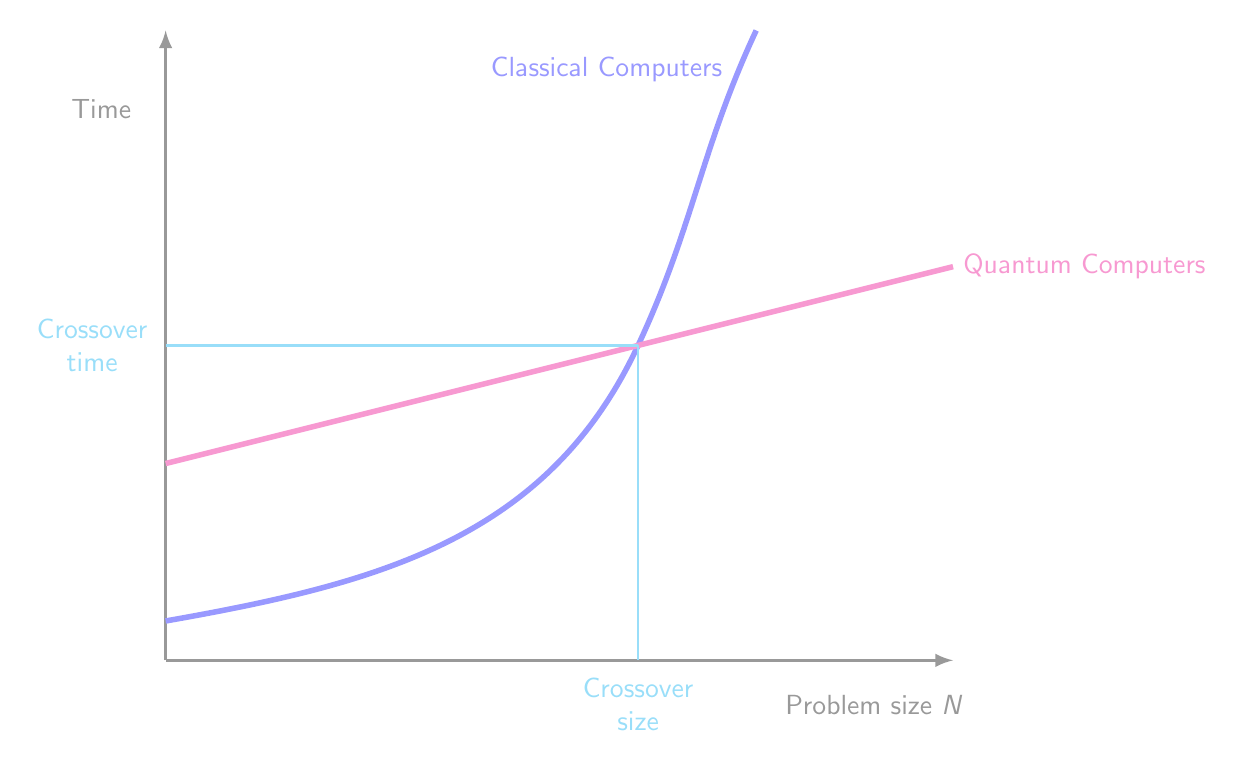
\begin{tikzpicture}[>=latex, thick, font=\sffamily]

% --- Axes ---
\draw[->, very thick, black!40] (0,0) -- (10,0) node[below, xshift=-1cm, yshift=-0.3cm] {Problem size \textit{N}};
\draw[->, very thick, black!40] (0,0) -- (0,8) node[left, xshift=-0.3cm, yshift=-1cm] {Time};

% --- Intersection Point ---
% Defined explicitly so all lines pass through it
\coordinate (crossover) at (6, 4);

% --- Curves ---

% 1. Classical (Exponential, dark blue)
% "out=10" starts flat. 
% "in=245" enters the crossover steeply from the bottom.
% "out=85" leaves the crossover almost vertically (very steep).
% "in=265" arrives at the top, keeping that steepness (no flattening).
% Classical (Blue) - Exponential Growth
\draw[blue!40, line width=2pt] (0, 0.5) 
    to[out=10, in=245] (crossover) 
    to[out=65, in=245] (7.5, 8);
\node[blue!40, left] at (7.2, 7.5) {Classical Computers};

% 2. Quantum (Linear, golden yellow)
% Calculated to pass exactly through (6,4). 
% Starts at (0, 2.5). Slope is 0.25.
\draw[magenta!40, line width=2pt] (0, 2.5) -- (10, 5);
\node[magenta!40, right] at (10, 5) {Quantum Computers};

% --- Crossover Lines and Labels ---
% Vertical line for crossover size
\draw[cyan!40, thick] (crossover) -- (6,0);
\node[cyan!40, below, align=center] at (6, -0.1) {Crossover\\size};

% Horizontal line for crossover time
\draw[cyan!40, thick] (crossover) -- (0, 4);
\node[cyan!40, left, align=center] at (-0.1, 4) {Crossover\\time};
\label{ch2:quantum adv}
\end{tikzpicture}

\caption{Classical vs Quantum Computers' performance on large problems}
\label{ch2:quantum adv}
\end{figure}

A key difference between quantum and classical computers is that quantum computers use qubits instead of traditional bits. Qubits are quantum particles that have special properties, the main one being superposition \cite{superposition}. Superposition means that a qubit can exist in multiple states simultaneously, with a probability of both states as shown in \ref{bit vs qubit}. So, if a qubit has a probability of being one and a probability of being zero, then it is in a state of superposition.
\usetikzlibrary{positioning, shadings, fadings}

% --- Define custom colors to match the image ---
\definecolor{cyan}{RGB}{255, 170, 0}   % A rich orange
\definecolor{blue}{RGB}{90, 150, 255}    % A bright blue
% Colors for the qubit gradient
\definecolor{cyan}{RGB}{255, 200, 80} 
\definecolor{blue}{RGB}{130, 210, 255}
\begin{figure}[ht]
\begin{tikzpicture}[font=\sffamily\bfseries, node distance=0.5cm]

    % =======================
    % LEFT SIDE: Classical Bit
    % =======================
    \begin{scope}[xshift=-4cm]
        % Title
        \node[align=center, font=\sffamily\mdseries] (bit_title) at (0, 4) 
            {\textbf{\LARGE Bit} \\[-0.3em] \textit{(Classical Computing)}};

        % '0' State
        \node[text=magenta, font=\huge] (bit_0_label) at (0, 2.5) {0};
        % Small orange sphere using ball shading
        \shade[ball color=magenta] (0, 1.3) circle (0.4cm);

        % '1' State
        % Small blue sphere
        \shade[ball color=blue] (0, -1.3) circle (0.4cm);
        \node[text=blue, font=\huge] (bit_1_label) at (0, -2.5) {1};
    \end{scope}


    % =======================
    % RIGHT SIDE: Quantum Qubit
    % =======================
    \begin{scope}[xshift=4cm]
        % Title
        \node[align=center, font=\sffamily\mdseries] (qubit_title) at (0, 4) 
            {\textbf{\LARGE Qubit} \\[-0.3em] \textit{(Quantum Computing)}};

        % '0' State Label
        \node[text=magenta, font=\huge] (qubit_0_label) at (0, 2.5) {0};

        % --- The Large Qubit Sphere ---
        \begin{scope}[yshift=0cm]
            % 1. Main body with a vertical gradient (orange -> white -> blue)
            % 'shading angle=0' makes the gradient vertical.
            \shade[
                top color=magenta, 
                bottom color=blue, 
                middle color=white, 
                shading angle=0
            ] (0,0) circle (1.8cm);
            
            % 2. Add a top highlight for a 3D, glossy effect
            % This is a white ellipse that fades out towards the bottom.
            \fill[white, opacity=0.5, path fading=south] 
                (0, 0.4) ellipse (1.8cm and 0.7cm);
        \end{scope}

        % '1' State Label
        \node[text=blue, font=\huge,] (qubit_1_label) at (0, -2.5) {1};
    \end{scope}
\label{bit vs qubit}
\end{tikzpicture}

\caption{Classical Bits vs Qubits}
\label{bit vs qubit}
\end{figure}

This state can be written according to the following equation \eqref{ch2:superpos_equ}:

\begin{equation}
    |\psi\rangle = \alpha |0\rangle + \beta |1\rangle
    \label{ch2:superpos_equ}
\end{equation}

\noindent Where:
\begin{itemize}
    \item $|\psi\rangle$ represents the state of the qubit.
    \item $|0\rangle$ and $|1\rangle$ are the zero and one states .
    \item $\alpha$ and $\beta$ are complex probability amplitudes.
\end{itemize}

Since $\alpha$ and $\beta$ are complex numbers, the probabilities are calculated by the squared magnitudes, as in Equation \eqref{ch2:prob_equ}:

\begin{equation}
    P(0) = |\alpha|^2 \quad \text{and} \quad P(1) = |\beta|^2
    \label{ch2:prob_equ}
\end{equation}
However, when these qubits are measured, they collapse into a classical deterministic state of one or zero, turning them into a classical bit that can then be manipulated using classical computers.
\newline 
This superposition property is the basis of quantum parallelism. Parallelism refers to the ability of a quantum computer to evaluate a function on many different inputs simultaneously; this results in quantum circuits processing a large number of possible values in parallel. However, a quantum computer does not return all the answers at the end. When the qubits are measured, they collapse to a single outcome. Hence, quantum algorithms must be designed to be used to amplify the probability of correct answers while suppressing incorrect ones so that when measurement occurs, the single result obtained is the best \cite{quantumparr}.

Another interesting property of these particles is entanglement, which essentially means that two particles become linked, so measuring one particle reveals information about the other, even if they are an infinite distance apart.
\\
    \textbf{Interference} \\ % Bold the title and add a line break
    Quantum states behave like waves, constructively and destructively, allowing quantum computers to process many possibilities in parallel.
\\
One of the characteristics that affects qubits negatively is decoherence; this is when a qubit collapses into a non-quantum state, either because of environmental factors or because it stays in the qubit state for a long time before being measured. If this characteristic is not taken into consideration when creating the quantum system, qubits may collapse long before we expect them, producing invalid results.

These principles work together by first preparing a superposition of computational states. Entanglement principles are then used in the quantum circuit prepared by the user to entangle qubits as seen in \ref{entagngle cir} and generate interference patterns governed by the quantum algorithm. Interference cancels out the many possible outcomes that are generated and amplifies others. The latter outcomes are the solution to the problem\cite{ibmQuantum}.

\subsection{Quantum Technologies}
Just as classical computers use logical gates to manipulate bits to produce desired results, quantum computers employ a similar system known as quantum gates. These gates may be one or 2 qubit gates. There are many quantum phenomena, such as:
\begin{itemize}
    \item  Pauli-X Gate ($X$): Serves as a traditional NOT gate. It switches $|0\rangle$ to $|1\rangle$ and vice versa.
\end{itemize}
\begin{itemize}
    \item Pauli-Y Gate ($Y$): This gate rotates the qubit around the Bloch sphere's Y-axis.
\end{itemize}
\begin{itemize}
    \item Pauli-Z Gate ($Z$): Phase-flips the qubit by rotating it around the Z-axis. 
\end{itemize}
\begin{itemize}
    \item Hadamard Gate ($H$): The most vital gate for creating superposition. It transforms a deterministic state of $|0\rangle$ or $|1\rangle$ into an equal superposition of both $|+\rangle$ or $|-\rangle$.
\end{itemize}
\begin{itemize}
    \item CNOT (Controlled-NOT) Gate ($CX$): Flips the target qubit if and only if the control qubit is $|1\rangle$. This is the primary gate used to entangle two qubits.
\end{itemize}
However, adding too many gates makes the operation take longer, causing the qubits to decohere. Thus, this issue should be taken into consideration when constructing the circuit.
\begin{figure}
\centering
    \begin{quantikz}
        \lstick{\ket{q_0}} & \gate{H} & \ctrl{1} & \qw \\
        \lstick{\ket{q_1}} & \qw      & \targ{}  & \qw
    \end{quantikz}

    \caption{Entangling circuit}
        \label{entagngle cir}

\end{figure}
The following circuit, shown in figure \ref{entagngle cir}, is used to entangle two qubits together.
\subsubsection{{Qiskit}}
Qiskit is an open-source Software Development Kit that contains tools that allow users to build, modify, and run quantum computer programs, enabling them to work at the level of quantum circuits and operators. It acts as an interface between quantum hardware and classical programming.
The basic components of Qiskit are:

\begin{itemize}
    \item Circuit-building tools: Used to create quantum gates, registers, and instructions.

\end{itemize}
\begin{itemize}
    \item Transpiler: A program designed to optimize the performance of general quantum circuits and map them to certain physical hardware.
\end{itemize}
\begin{itemize}
    \item Quantum Info Library: A mathematical toolkit for noise-free calculations, including quantum states and operators.
\end{itemize}
\paragraph{Qiskit Runtime}
\mbox{} \\
This is a cloud-based service that allows users to execute quantum tasks on real IBM Quantum Hardware. This service utilizes a containerized environment to run them at the hardware level, making it more efficient. It provides primitives such as :
\begin{itemize}
    \item Sampler:  Starts by executing the quantum circuit, measures its results, and sends the list of probabilities of different outcomes back to the user's computer.
\end{itemize}
\begin{itemize}
    \item Estimator: Unlike the sampler, the estimator calculates the expected value from the circuit and returns it.

\end{itemize}

This service also has built-in methods for error suppression, which are applied during execution to avoid errors occurring. Also, it has error mitigation, which is applied after execution to correct the errors that took place.
\\
Job submissions to the quantum servers can be done in 3 ways \cite{qiskiteco}:
\begin{itemize}
    \item Job mode: Submits a single run.

\end{itemize}
\begin{itemize}
    \item Session mode: Allows for multiple iterative jobs.

\end{itemize}

\begin{itemize}
    \item Batch mode: Submits multiple jobs in parallel.

\end{itemize}
\paragraph{Qiskit Aer}
\mbox{} \\
This package's goal is to provide high-performance simulations of real quantum computers. It is used so users can test their circuits locally on their devices before sending them to IBM’s quantum servers. To ensure it is realistic, the aer package allows users to choose the exact real quantum chip they want to use, and then it simulates the errors based on the device properties and noise of that chip. This allows users to simulate their circuit on various chips and see which one gives optimal results before executing it on real quantum devices.

\subsubsection{{Quantum Optimization}}
As mentioned earlier, quantum computers are used for solving optimization problems due to quantum parallelism. However, to be able to execute these problems on quantum computers, they must first be formulated as a Quadratic Unconstrained Binary Optimization (QUBO) problem. In a QUBO model, the decision variables are binary.  The objective is expressed as a quadratic polynomial, where Q is the matrix that represents how variables interact, and c is the cost or penalty for each variable, as seen in \ref{qubo}:
\begin{equation}
    f(x) = x^\top Q x + c^\top x
    \label{qubo}
\end{equation}

This formulation allows infeasible solutions to be eliminated by assigning them high costs.
The problem can be reformulated as an Ising Hamiltonian once it has been expressed as a QUBO. The optimization problem is changed to an energy minimization problem in the Ising model using the  equation \ref{hamiltion}:
\begin{equation}
    x = \frac{1 - Z}{2}
\label{hamiltion}
\end{equation}


where $x \in \{0,1\}$ is a binary decision variable and $Z$ is the Pauli-$Z$ operator.

The Quantum Approximate Optimization Algorithm (QAOA) can then be applied.


QAOA is a technique that solves optimization problems using both a classical computer and a quantum computer. QAOA prepares a probability distribution over states at once and repeatedly modifies them to increase the possibility of better ones. We measure the circuit after a few rounds and look at the most common solutions, which are usually good solutions. Although QAOA is intended to find strong approximations on modern quantum devices, it does not always provide the exact answer.



The cost Hamiltonian, denoted by $H_C$, encodes the cost function and penalties of the optimization problem. Lower energy values represent lower cost solutions. In the QAOA framework, $H_C$ is applied through \ref{hc unitary}:
\begin{equation}
U(H_C, \gamma) = e^{-i \gamma H_C}
\label{hc unitary}
\end{equation}

To implement this on a quantum processor, the operator is decomposed into a series of gates as seen in \ref{hc gates}:

\begin{equation}
U(H_C, \gamma) = \prod_{i<j} e^{-i \gamma J_{ij} \hat{Z}_i \hat{Z}_j} \prod_{i} e^{-i \gamma h_i \hat{Z}_i}
\label{hc gates}
\end{equation}
\begin{itemize}
    \item $\gamma$: A parameter determined by the classical computer.
  \item $\hat{Z}_i$: A quantum operator that checks if a qubit is in state $0$ or $1$( in the VRP problem, this checks if a certain location is in my route).
    \item $J_{ij}$: The cost associated with the relationship between two variables, such as the travel cost between location $i$ and location $j$.
    \item $h_i$: The specific cost assigned to a single decision, such as a service fee at a specific stop or a fixed vehicle activation cost.
\end{itemize}




The Hamiltonian of the mixer, denoted by $H_M$, is responsible for exploring the search space, preventing the algorithm from getting stuck in a local minima by driving rotations using  the $\hat{X}$ operator (the Pauli-$X$ gate)as seen in \ref{hm unitary}:

\begin{equation}
U(H_M, \beta) = e^{-i \beta H_M}
\label{hm unitary}
\end{equation}
Expanding this into single-qubit rotations as used in the quantum circuit:
To implement this on a quantum processor, the operator is decomposed into a series of gates as seen in \ref{hm gate}:
\begin{equation}
U(H_M, \beta) = \prod_{i=1}^{n} e^{-i \beta \hat{X}_i}
\label{hm gate}
\end{equation}


\begin{itemize}
    \item $\beta$: A parameter determined by the classical computer.
    \item $\hat{X}_i$: The Pauli-$X$ operator acting on the qubit $i$.
    \item $n$: The total number of qubits.
\end{itemize}
Both Hamiltonians depend on two variational parameters, $\beta$ and $\gamma$, which are
iteratively optimized by a classical computer.

\paragraph{QAOA Procedure as shown in figure \ref{qaoa}:}
\begin{figure}
    \centering
    \includegraphics[width=1\linewidth]{Images/qaoa cicuit1.png}
    \caption{QAOA Circuit}
    \label{qaoa}
\end{figure}
\begin{enumerate}
    \item Initialize all qubits in the superposition state $|+\rangle$,
    representing all possible solutions simultaneously.
    \item Apply  layers of the cost Hamiltonian and the mixer Hamiltonian,
    repeated $p$ times, where increasing $p$  improves the accuracy of the solution.
    \item A classical optimizer measures the quantum state, evaluates the cost, and
    updates the parameters $\beta$ and $\gamma$.
    \item After convergence, the circuit is measured multiple times. The most frequent bitstring corresponds to the best solution.
\end{enumerate}

QAOA has multiple advantages that make it suitable for combinatorial optimization problems such as VRP. It naturally supports problems expressed in QUBO form; constraints such as capacities, time windows, and route penalties can be incorporated into the cost Hamiltonian, allowing flexible modeling of the problem. In addition, it integrates well with gate-based quantum hardware and works effectively on NISQ. devices. 

However, QAOA also has limitations. The algorithm must be executed repeatedly, tuning parameters, and the quality of the final solution depends on the selection of penalties, circuit depth, and the number of layers. Furthermore, as the problem grows larger, performance may degrade due to the limited qubits available on current devices. Despite these challenges, QAOA is adopted in this work as the primary quantum optimization approach.
% optimizer



\section{Literature Review}
\subsection{Classical approaches}

As the VRP problem scales, it becomes increasingly hard and expensive to calculate the optimal solution. To resolve this, heuristic and metaheuristic techniques emerged. These techniques focus on finding a good solution, but not necessarily the optimal one, by using guided randomness.
\subsubsection{Heuristics}
In a paper called Heuristics for Vehicle Routing Problem: A Survey and Recent Advances \cite{heuristics}, the authors analyzed multiple methods that researchers approached the VRP problem with. The authors classified  heuristic approaches into 3 different categories:
\begin{itemize}
    \item \textbf{Constructive Heuristics:} These algorithms build the solution from scratch. They may be fast, but they don't always provide the optimal result, for example:
    
    \begin{itemize}
        \item \textbf{Nearest neighbors :} It adopts a greedy approach.
        
        \item \textbf{Insert method:} Creates empty routes, then adds customers where they result in a minimum cost increase.
        
        \item \textbf{Saving method, also known as the Clarke-Wright method:} Starts by assigning one vehicle per customer, then merges the routes that result in maximum savings in distance.
        
        \item \textbf{Sweep method:} \\
        Sorts the locations by their angle from the depot, then clusters them
    \end{itemize}
\end{itemize}
\begin{itemize}
    \item Improvement heuristics, also known as local search:

These algorithms take existing solutions and attempt to improve them using either

1 - Intra-route, which uses methods like reversing the order of nodes in a route.

2 - Inter-route, which uses methods like swapping customers from one route to another.


\end{itemize}
\begin{itemize}
    \item Metaheuristics

This type is mainly known for its avoidance of getting stuck in local optima. This can be done by improving a single solution or by evolving a set of them, as will be discussed in the next subsection.
\end{itemize}

\subsubsection{Metaheuristic}


A paper in 2018 used reinforcement learning to solve the CVRP \cite{metavrp}. This paper focused on building a simple model with static embedding and an RNN decoder with attention mechanisms. This technique allowed the policy to update without the need to reconstruct the whole network. This model was trained using the policy gradient method. This helped make it more efficient for nodes between 50 and 100, surpassing the heuristic Clarke-Wright and Google OR-tools in terms of solution quality and computation time.

Another approach used in a recent paper was the genetic algorithm approach, which simulates natural selection to evolve a population. The authors encoded the problem into chromosomes using permutations of customers' visits. They also used the inverse of the distance as the fitness function to evaluate the quality of this solution. Some of the methods used to simulate the genetic algorithm were
\begin{itemize}
    \item Selection: This way is done using methods like the roulette wheel to choose parents based on their fitness.
\end{itemize}
\begin{itemize}
    \item Crossover: This method was used to create offspring combining traits from both parents while maintaining valid routes, utilizing operators such as Order Crossover (OX) or Partially Mapped Crossover (PMX). 
\end{itemize}
\begin{itemize}
    \item Mutation: Random changes to maintain diversity and ensure not getting stuck in local optima. 
\end{itemize}

This approach resulted in flexibility, which was a necessity to handle constraints like time windows, and was scalable. However, this method faced issues when it came to parameter tuning.\cite{genvrp}

Müller and Meira \cite{muller2018genetic} applied a genetic algorithm to a real-world Brazilian mail delivery benchmark, comparing BCR and OX crossover operators combined with 2-opt local search across instances with up to 30,000 delivery locations. Their results showed that BCR with local search consistently outperformed other configurations, and that route length variance — used as a fairness metric — was best reduced when local search was enabled in which the authors optimize for multiple parameters: the number 
of vehicles ($K$), route length, and the unfairness of the workload 
distribution among mailmen. The benchmark itself, introduced by Meira et al. \cite{meira2018postvrp}, models mail delivery in the city of Artur Nogueira, Brazil, and addresses the lack of large-scale real-world VRP datasets, offering significantly more delivery locations than classical sets such as TSPLib or Solomon's benchmark.

\subsection{Quantum approaches}
While classical algorithms rely on heuristics to navigate the solution space, quantum computing introduces a fundamental shift by leveraging quantum mechanical phenomena such as superposition and entanglement. Quantum algorithms aim to escape the local minima that often trap classical solvers by traversing the energy landscape via quantum tunneling, as shown in \ref{quantum tunneling} \cite{kadowaki1998quantum}.
\begin{figure}[ht]
\centering

% Define custom colors for a more aesthetic look
\definecolor{quantumgreen}{RGB}{219,112,147}
\definecolor{darkgrey}{RGB}{50, 50, 50}

\begin{tikzpicture}[>=Stealth, font=\sffamily]

    % --- 1. Define Key Coordinates ---
    % Adjusted coordinates to make the curve look more balanced
    \coordinate (start) at (0, 6.5);
    \coordinate (local_min) at (2.8, 3.0);
    \coordinate (peak) at (5, 6);
    \coordinate (global_min) at (7.5, 1.0);
    \coordinate (end) at (10.5, 7);

    % --- 2. Draw Axes ---
    % Increased the 'below' distance for the x-label to fix the overlapping issue
    \draw[<->, thick, color=darkgrey] 
        (0, 8) node[above, rotate=90, anchor=east, yshift=0.5cm, text=black] {\textbf{Cost of Energy}} 
        |- 
        (11, 0) node[below=0.8cm, anchor=north, xshift=-1cm, text=black] {\textbf{Solution / System Configuration}};

    % --- 3. Draw the Energy Landscape Curve ---
    % 'tension=0.9' makes the curve smoother and more fluid
    \draw[line width=2pt, color=black] plot [smooth, tension=0.9] coordinates { 
        (start) (local_min) (peak) (global_min) (end) 
    };

    % --- 4. Labels for Minima ---
    \node[below=0.2cm, color=darkgrey] at (local_min) {Local Minima};
    \node[below=0.4cm, color=darkgrey] at (global_min) {Global Minima};

    % --- 5. Simulated Annealing (Thermal Jump) ---
    % A curved arrow jumping over the peak
    \draw[->, thick, color=black!80, bend left=65] 
        ($(local_min) + (0.0, 2.5)$) to 
        node[above=0.1cm, align=center, font=\small] {Simulated Annealing\\(Thermal Jump)} 
        ($(global_min) + (-0.2, 4.0)$);

    % --- 6. Quantum Tunneling (Green Arrow) ---
    % I shortened the arrow (made it "smaller") by adding offsets to the start/end coordinates
    % so it sits neatly inside the barrier.
    \draw[->, line width=3pt, color=quantumgreen] 
        ($(local_min) + (1, 0.8)$) -- ($(global_min) + (-1.5, 2.8)$)
        node[midway, below=0.35cm, align=center, font=\scriptsize] {Quantum Annealing\\(Tunneling)};

\end{tikzpicture}
\caption{Simulated Annealing vs Quantum tunneling }
\label{quantum tunneling}
\end{figure}
\newline
\indent To utilize current quantum hardware, the VRP must be reformulated from its standard programming representation into a format compatible with quantum architectures. The most prevalent method is to map the problem to a Quadratic Unconstrained Binary Optimization (QUBO) model or an Ising Hamiltonian. As detailed by Lucas\cite{lucas2014ising}, NP-hard problems like the Traveling Salesman Problem (TSP) and VRP can be encoded into an energy function where the lowest energy corresponds to the optimal route.
\newline
\indent The most experimentally mature approach for routing problems is Quantum Annealing, primarily utilizing D-Wave Systems. Unlike universal gate-based models, QA is specialized for optimization. Feld et al. \cite{feld2019hybrid} demonstrated one of the first successful applications of Quantum Annealing to the Capacitated Vehicle Routing Problem. Their work highlighted that while the annealer could effectively solve small instances, the topology often requires "minor embedding," which significantly increases the overhead required to represent fully connected graphs.
\newline
\indent On universal quantum computers, the Quantum Approximate Optimization Algorithm (QAOA), introduced by Farhi et at. \cite{farhi2014quantum}, serves as the standard meta-heuristic.\newline QAOA is a variational algorithm that uses classical optimizers to tune the parameters of the quantum circuit to minimize the cost function. While it's theoretically capable of achieving a quantum advantage, Vikstål et al. \cite{vikstal2020applying} note that applying QAOA to routing problems is currently hindered by the depth of the quantum circuits that are required, and as the problem size increases, the noise accumulates, degrading the quality of the solution before the algorithm can converge.
\newline
\indent Current research acknowledges that we are in the "Noisy Intermediate-Scale Quantum" (NISQ) era, a term coined by Preskill \cite{preskill2018quantum}. In this stage, quantum processors are bound by a low qubit count and high error rates. Osaba et al. \cite{osaba2021hybrid} provide a review of quantum optimization in logistics, concluding that pure quantum solvers are currently restricted to "toy problems" containing fewer than 100 nodes.
\newline
\indent Consequently, to address the scale of real-world problems and benchmarks while leveraging the advantages of quantum search, researchers have pivoted towards hybrid approaches. These systems, discussed in the next section, divide large problems into smaller sub-problems, suitable for quantum processing.
\subsection{Hybrid approaches}
The term "hybrid" refers to a combination of both classical and quantum systems that are used side-by-side to leverage the advantages of both: control, optimization, and data handling for classical computers, as illustrated in \ref{vqe}. While the quantum computer handles harder and more specific parts of the problem. This is specifically useful in the current NISQ(Noisy Intermediate-Scale Quantum) era since quantum computers cannot run long algorithms due to noise and limited qubit count\cite{howvqe}.

\begin{figure}
\centering
    \includegraphics[width=0.7\textwidth]{Images/vqe.jpeg} 
    \caption{Feedback Loop in VQE.}
        \label{vqe}

\end{figure}
Many hybrid quantum-classical algorithms can be used to get the most out of quantum computers, with the Variational Quantum Eigensolver (VQE) being "the gold standard". It consists of four main components: 
\begin{itemize}
    \item Quantum Processor that executes the parametrized circuit and performs measurements
    \item Classical Optimizer that tunes the circuit parameters to minimize energy.
    \item Ansatz, which is a parametrized quantum circuit that is essentially the blueprint for a trial quantum state.
    \item Hamiltonian, which is the operator whose lowest eigenvalue, or ground state energy, we seek.
\end{itemize}
The VQE aims to find the optimal parameters classically by calculating the ground state through iteratively refining the ansatz, and comparing each new result with the previous one until it converges near the true ground state.
This can be achieved through the following process: 
\begin{quote}
    First, the system is represented as a Hamiltonian operator (H), which describes the total energy.
\end{quote}
\begin{quote}
     Second, we design the Anstaz circuit, which prepares a trial quantum state  \(|\psi (\theta )\rangle \), where $\theta$ represents the parameters.
\end{quote}
\begin{quote}
    The next step is where quantum execution happens. The ansatz circuit is run on the quantum computer to find the expectation value of the Hamiltonian.
\end{quote}
\begin{quote}
    The measured values are then used in classical optimization algorithms, on a classical computer, to adjust $\theta$ such that it gives the lowest energy value.
\end{quote}
\begin{quote}
    The two previous steps are repeated until the energy converges to a minimum.\cite{vqe}\cite{howvqe}
\end{quote} 
\begin{center}
    
\end{center}

Recent surveys emphasize that this modular structure is the primary enabler for quantum utility in the NISQ era. Offloading parameter updates to classical hardware gives the hybrid algorithms the chance to harness classical robustness to mitigate quantum hardware limitations, like short coherence times\cite{hybrid}.
Other works have demonstrated that replacing classical optimizers with Deep Neural Networks can accelerate the feedback loop between the classical and quantum computers, allowing for faster prediction of optimal parameters as compared to the conventional gradient-based methods\cite{DRL}.
\newline
The Ansatz is the most researched part of the VQE. Its quality, structure, and initial parameters significantly impact the accuracy and efficiency of the algorithm. Designing an effective Anstaz is a crucial step that can be challenging for complex problems. It must be expressive enough to reflect the important features of the target state, but not too complicated that its implementation on a quantum computer becomes impossible\cite{ansatz}. The trainability of the Ansatz has a direct effect on the algorithm's ability to converge.
\newline
Traditional research has been centered around the Unitary Coupled Cluster family of operators due to their rigorous grounding in electronic structure theory\cite{ucc}. However, these circuits are often so deep that they exceed the coherence times of current hardware. For that reason, current research has shifted towards adaptive algorithms like ADAPT-VQE, which dynamically construct the Ansatz by adding more operators that maximize the energy gradient. The operators used are guaranteed to be the ones necessary to construct an exact ansätze\cite{adaptvqe}.
\newline
The huge impact of the Ansatz on the VQE comes from its ability to explore wide solution spaces that are appropriate to the problem, which ultimately decides how close the algorithm can get to finding an approximate true solution to the given problem.
The challenge is to find a balance between how expressive and how trainable the ansatz is. Multiple works have explored automated designs of the Ansatz to improve the performance of the algorithm. Methods like genetic algorithms and gate-level optimization aim to optimize circuit design using search heuristics\cite{automatedansatzdesign}. Policy-driven agents in deep reinforcement learning are employed to search these quantum architectures by accessing Pauli-X, Y, Z expectation values and a predefined set of quantum operations for learning the target quantum state. It is optimized by the Advantage Actor-Critic and Proximal Policy Optimization algorithm\cite{reinlearnagents}. 
\newline
Quantum architecture search, a resource and runtime-efficient scheme, automatically seeks a near-optimal circuit architecture(ansatz) to balance benefits and side-effects that result from adding more noisy quantum gates to improve performance\cite{qarchsearch}.
\newline
Throughout the years, the literature has shifted from purely theoretical proofs to practical applications in different industries. In the financial sector, the use of VQE-based methods for Portfolio Optimization has attracted many in that sector. The objective function uses binary variables to represent buy/hold/sell decisions to balance the return against risk, like Conditional Value at Risk\cite{portfolioptim}.
\newline
The logistics sector has also employed hybrid models to prevent parts from running out and dynamically balance supplier options. Fleet maintenance, cargo loading, prediction, and scheduling through VQE-based methods were optimized in such a way that reduces costs and utilizes resources\cite{logisticsvqe}.

\subsection{Fairness Metrics}
Different fairness measures have been used across the literature for different purposes.

\subsubsection{Standard Deviation $\sigma$}
It captures the average deviation of each route from the mean, expressed in the same units as distance. $\sigma$ is sensitive to all routes, not just the extremes, and is well established multi-objective VRP \cite{standardDev}, making it fit for the work presented here. 
However, when a route is shorter than average, it is penalized the same way as one that is longer, even though in practice, the concern would be on the overloaded drivers.

\subsubsection{Coefficient of Variation}
It measures relative spread rather than absolute spread, so it reflects $\sigma$ as a percentage of the mean.
This approach is directly comparable across instances of different sizes and geographies, but cannot be directly combined with a distance-based cost term without introducing a normalization factor or arbitrary scaling\cite{cv}.

\subsubsection{Min-Max Ratio}
Captures how many times longer the longest route is compared to t






\subsection{Clustering Approaches}



\section{Summary}
The vehicle routing problem created by Dantzig and Ramser in 1959 is an optimization problem whose goal is to determine the most effective routes for a number of vehicles that serve a group of customers according to a cost function. This problem has extended to include multiple variants such as the CVRP and TWVRP. This problem is considered an NP-hard problem as the computational complexity increases exponentially with the increase in the number of vehicles and customers. Which results in the classical method falling short. 

To resolve this issue, quantum computers provide a solution to this by utilizing the laws of quantum mechanics, specifically superposition and entanglement. Unlike classical bits, which have deterministic states, a qubit can represent multiple states. This is useful as it enables quantum parallelism, evaluating a large number of routes at once, achieving quantum advantage in theory.

In order to achieve this advantage, many tools were developed, such as Qiskit, which acts as a bridge between classical and quantum computers, compiling high-level code into physical pulses that run on real quantum hardware using the cloud.

In addition to that, many techniques emerged, such as hybrid quantum-classical computing, which also utilizes classical computing to help error mitigation. This is necessary because current quantum processors are prone to noise and decoherence, making them unreliable for long, complex calculations on their own.
\chapter{Design}

\section{Analysis of Design Requirements}

 \begin{itemize}

  \item \textbf{The design shall include a minimum of two metrics to formulate
  the objective function of the VRP optimization problem:}
  In real-world delivery operations, optimizing for a single metric is
  insufficient to produce practically viable routes. A solution that minimizes
  total travel distance may still be operationally impractical if it
  concentrates deliveries on a subset of vehicles, leading to uneven workload
  distribution, driver fatigue, and delayed service. This requirement therefore
  mandates that the objective function be formulated using at least two distinct
  metrics total route distance and inter-vehicle workload fairness so
  that the optimization reflects the dual priorities of cost efficiency and
  operational balance simultaneously.

  \item \textbf{The design shall allow for both single-objective and
  multi-objective optimizations:}
  This requirement requires that the system support both optimization modes
  within a unified framework. The system is designed to address this through a
  hierarchical structure: at the quantum layer, the QAOA cost Hamiltonian
  formulates a single-objective QUBO that minimizes total route distance within
  each decomposed sub-problem. At the classical decomposition layer, a fairness
  criterion governing equitable workload distribution across vehicles is
  enforced globally across the full instance. The two objectives are therefore
  handled at distinct levels of the pipeline, constituting a multi-objective
  formulation without merging competing criteria into a single weighted term at
  the quantum stage.

  \item \textbf{The design shall generate valid and practical solutions by
  eliminating subtours using a minimum of two approaches:}
  A subtour is an invalid partial route in which a subset of delivery nodes is
  visited in a closed loop that never returns to the depot, rendering the
  solution infeasible. Subtours arise naturally in combinatorial QUBO
  formulations and must be actively suppressed. Since a single elimination
  mechanism may be insufficient in all problem configurations, particularly as
  instance size grows, this requirement mandates the use of at least two
  independent subtour elimination approaches to ensure solution validity is
  maintained across all tested instances.

  \item \textbf{A minimum of 2 VRP instances (of different sizes) shall be
  used for testing the proposed route optimization system:}
  Evaluating a route optimization system on a single instance provides no
  evidence of generalizability. Performance characteristics that hold for small
  instances may degrade significantly as customer count increases due to higher
  qubit requirements, deeper quantum circuits, or instability in the
  decomposition pipeline. This requirement mandates testing across at least two
  instances of meaningfully different sizes to ensure that the system's behavior
  is understood across a representative range of problem scales.

  \item \textbf{Route optimization shall be implemented on a real cloud-based
  quantum computer and compared to a minimum of one classical optimization
  approach:}
  Local simulation cannot reproduce the noise, decoherence, and gate-error
  conditions present on real quantum hardware, which are the primary practical
  constraints on near-term quantum optimization. This requirement mandates
  execution on a real cloud-accessed quantum device to ensure the system is
  evaluated under authentic hardware conditions. The additional requirement for
  a classical comparison ensures that the quantum solver's output is benchmarked
  against an established optimization baseline, providing a meaningful reference
  for evaluating solution quality.

  \item \textbf{The proposed system shall include a server application that
  hosts the delivery tasks, the optimized routes, and a client application
  for drivers and administrators:}
  A route optimization algorithm that operates only as an offline computational
  tool has limited operational value in a real logistics context. This
  requirement mandates a server application responsible for centrally hosting
  delivery tasks and serving optimized routes, and a client application
  providing role-specific interfaces drivers receive and view their assigned
  routes, while administrators manage tasks and oversee the full delivery
  pipeline.

  \item \textbf{The proposed system shall provide real-time route updates and
  monitoring, in addition to secure authentication and role-based access:}
  Optimized routes are of no operational value if they cannot reach drivers
  promptly and through a controlled process. This requirement mandates that
  once an administrator reviews and dispatches optimized routes, drivers receive
  their assignments immediately through the client application, without manual
  relay or delay between the dispatch action and delivery receipt. The
  administrator interface is responsible for reviewing computed routes,
  authorizing dispatch, and monitoring delivery progress, while the driver
  interface is limited to receiving and viewing assigned routes. Secure
  authentication ensures platform access is restricted to registered users,
  and role-based access control enforces the boundary between administrator
  capabilities and driver permissions, preventing unauthorized route modification
  or task management.

  \end{itemize}

\section{Analysis of Design Constraints }
The realistic constraints that are considered in the design process are explained in the following: 

\subsection{Manufacturability and Sustainability}
The project follows certain criteria to maintain the sustainability of the solution:

\begin{itemize}
    \item  The code is built in a scalable manner, using a modular architecture where the quantum solver, classical baselines, and visualization tools are independent, reusable components.
\end{itemize}
\begin{itemize}
    \item All main dependencies, including Qiskit, Qiskit-Aer, OR-Tools, and NumPy are
open-source frameworks, ensuring long-term adaptability without licensing costs.
\end{itemize}
\begin{itemize}
 \item The hybrid classical-quantum design further supports sustainability by confining quantum computation to small leaf sub-problems, making the system practical on
both simulated and real quantum backends.
\end{itemize}


\subsection{Economic Constraints}

The primary economic constraint arises from the cost of accessing quantum 
computing resources through cloud platforms. Services such as IBM Quantum (via 
Qiskit), AWS Braket, and D-Wave Leap charge either per execution shot or per second of QPU runtime, which directly limits the number of quantum circuit evaluations the project can afford.

To mitigate this, the project adopts the following cost-reduction strategies:

\begin{itemize}

    \item \textbf{Hybrid Classical-Quantum Decomposition:} The recursive solver 
    confines quantum computation (QAOA) exclusively to small leaf sub-problems of 
    at most \texttt{LEAF\_SIZE} nodes. The routing logic clustering, merging, post-processing, and baseline comparisons execute entirely on classical hardware at no cloud cost.

    \item \textbf{Local Simulation First:}During the design and testing stages Qiskit-Aer’s statevector simulator running locally was used, to reduce cloud charges.
 
\end{itemize}
These choices ensure that the project remains executable within a constrained budget while still solving a realistic problem instance.


\section{Discussion of Engineering Standards }
\begin{itemize}
    \item Following ISO/IEC 25010 standards:
    \begin{itemize}
        \item The QUBO formulation and classical optimizer in the QAOA loop were chosen to maximize performance efficiency (Time Behavior \& Resource Utilization).
        \item The codebase is modular to accommodate changes in quantum backends without restructuring the core logic.
        \item A systematic code review was performed, catching critical bugs and ensuring the reliability of the system.
    \end{itemize}
    \item Following IEEE 829 principles:
    \begin{itemize}
        \item Hyperparameter sweeping was structured as a formal test to find optimal configurations for reps, optimizer, and iteration count.
        \item The system was tested across varying node sizes and multiple random seeds, confirming the solver generalizes across problem sizes.
    \end{itemize}
\end{itemize}
\section{Different Design Approaches} 
While designing this project, multiple design choices were taken into consideration, such as: 

\subsection{Framework Choice}
Many quantum frameworks are available, each with different simulator capabilities, hardware access pathways, and degrees of manual circuit construction required. The three most widely used open-source frameworks are IBM's Qiskit, Xanadu's PennyLane, and Google's Cirq. The following subsections compare them across three criteria: algorithm and optimization support, simulation and hardware access, and community support.
Qiskit is a full-stack quantum computing framework covering algorithm specification, circuit compilation, simulation, and execution on real hardware, while PennyLane was built specifically for quantum machine learning, with automatic differentiation of quantum circuits as its central design feature. Cirq, on the other hand, is primarily a circuit construction and execution tool developed for Google's NISQ hardware. It operates at a lower level of abstraction with no native higher-level algorithm library beyond what a user constructs manually.
\subsubsection{Algorithm and Optimization Problem Support}
The most critical requirement for this project was the ability to encode a combinatorial optimization problem as a Quadratic Unconstrained Binary Optimization (QUBO) instance and automatically construct the corresponding QAOA circuit. Qiskit provides this through the \textit{qiskit-optimization} library, which implements a complete pipeline. \textit{QuadraticProgram} accepts linear and quadratic objective terms with equality constraints and converts them to a QUBO. The result is then mapped to an Ising Hamiltonian via  \textit{to\_ising},from which \textit{QAOAAnsatz} constructs a parametrized circuit directly. The \texttt{qiskit-algorithms} library further provides native implementations of ADAM, COBYLA, and SPSA optimizers that interface directly with the Estimator primitive, enabling multi-configuration sweeps over optimizer settings without additional adapter code.

PennyLane supports QAOA through its \textit{pennylane.qaoa} module and is competitive for gradient-based variational approaches, but the QUBO-to-circuit encoding pipeline requires substantially more manual construction compared to Qiskit's integrated SDK. Cirq provides no native QAOA or combinatorial optimization library; any implementation must be built from scratch at the gate level, which would have imposed an unreasonable development overhead for this project.
\subsubsection{Simulation and Hardware Access}
Qiskit Aer provides multiple simulation backends with noise modeling capabilities. Qiskit integrates natively with IBM Quantum hardware through the Runtime service, with managed access to processors exceeding 100 qubits, built-in error mitigation, and session management.
PennyLane can use Aer as an external plugin backend but runs slower on circuits of comparable depth and qubit count. Its plugin architecture supports backends from multiple vendors, offering hardware flexibility at the cost of hardware-specific optimization depth. Cirq's noise models are calibrated to Google's Sycamore architecture and do not generalize to other hardware configurations. Its hardware access is restricted to Google Quantum AI systems, which are not publicly available at scale and require direct Google collaboration.
\subsubsection{Community and Support}
Qiskit has the largest community of the three frameworks by documentation breadth and academic adoption. It includes a peer-reviewed textbook, structured learning courses, and the most active Stack Overflow presence among quantum computing frameworks. For a research project requiring rapid debugging of framework-specific behavior, this is a practical advantage that PennyLane and Cirq do not match at the same scale.


Qiskit was selected for this project for three reasons. First, its \textit{qiskit-optimization} library provides the only integrated QUBO-to-QAOA pipeline among the three frameworks, eliminating the need for manual circuit construction at the gate level. Second, native integration with IBM Quantum hardware through the Runtime service was essential for executing circuits on real quantum processors. Third, its documentation and community support make the development easier throughout the implementation. 

\subsection{QUBO Formulation}
Before any quantum algorithm can be applied to a routing problem, the problem 
must be translated into a form that the quantum hardware can work with. This translation is done through Quadratic Unconstrained Binary Optimization (QUBO), where every decision in the problem gets assigned a binary 
variable ($x_i \in \{0, 1\}$), and the total cost is expressed through 
linear and quadratic interactions between those variables. Since quantum hardware naturally seeks the lowest-energy ground state, the QUBO is built so that the lowest-energy state corresponds exactly to the optimal routing solution. Constraints are handled by algebraic penalty terms that push the energy of any invalid configuration higher, steering the optimizer away from infeasible routes.

The five QUBO formulations for the Traveling Salesman Problem (TSP) and Vehicle 
Routing Problem (VRP) identified in the literature are:

\begin{enumerate}
    \item \textbf{Position-Based TSP Formulation}
    This is the most qubit-efficient option, though it is limited to single-vehicle instances. The position index $t$ has no way to distinguish between multiple vehicles 
    occupying slots simultaneously \cite{bermejo2022gps}.
    \begin{itemize}
        \item \textbf{Approach}: Each city $i$ is mapped to a sequence slot $t$ 
        through the variable $x_{i,t}$, as shown in \ref{postion based}.
        \item \textbf{Logic}: The mapping is purely positional. To calculate travel 
        costs, the objective function uses terms that capture movement 
        between consecutive slots $t$ and $t+1$.
        \item \textbf{Subtour Handling}: Subtours are prevented by construction, 
        but only because the one-hot constraints are strictly enforced. Penalty 
        terms are added so that every row and column of the $x_{i,t}$ matrix 
        sums to exactly 1 — each position holds exactly one city, and each city 
        occupies exactly one position.
        \item \textbf{Qubit Count}: Requires exactly $N^2$ variables, where $N$ 
        represents the number of cities, excluding the depot.
    \end{itemize}
    \begin{figure}
        \centering
        \includegraphics[width=0.6\linewidth]{Images/Chapter 3/Qubo part/postion based.png}
        \caption{A visualization of the QUBO for TSP position-based encoding.}
        \label{postion based}
    \end{figure}

    \item \textbf{Edge Encoding (Edge without Time)}
    A standard topological approach that appears frequently in hybrid 
    quantum-classical decomposition strategies \cite{maciejunes2025solving}.
    \begin{itemize}
        \item \textbf{Approach}: Rather than tracking positions or time, this 
        formulation assigns one qubit to every potential edge in the graph directly.
        \item \textbf{Logic}: The binary variable $x_{ij}$ is simply 1 if that 
        edge is used in the final route, and 0 otherwise. Degree constraints 
        enforce that every customer node has exactly one incoming and one outgoing 
        edge ($in=1, out=1$), while the depot must have exactly $k$ of each 
        ($in=k, out=k$) to accommodate multiple vehicles.
        \item \textbf{Subtour Handling}: Degree constraints alone are not enough 
        to prevent subtours; disconnected loops can still satisfy them. Subtour 
        elimination must be handled separately through additional penalty terms.
        \item \textbf{Qubit Count}: Requires $N^2 - N$ qubits, where $N$ including the depot.
    \end{itemize}
    
    \item \textbf{General Edge with Time Native Formulation}
    This is the most commonly referenced formulation in quantum routing 
    literature \cite{bermejo2022gps}.
    \begin{itemize}
        \item \textbf{Approach}: Instead of just knowing which edges are used, 
        this formulation also tracks when. The variable $x_{u,v,t}$ records 
        which edge $(u,v)$ is traversed at each time-step $t$.
        \item \textbf{Logic}: Time here is sequential order (step 1, step 2, 
        step 3) and each step can only have one active edge.
        \item \textbf{Subtour Handling}: Because only one edge can be active per 
        time step and the progression is strictly forward, subtours cannot form. 
        \item \textbf{Qubit Count}: Requires $N^2(N-1)$ variables, where $N$ is the 
        number of cities including the depot.
    \end{itemize}

    \item \textbf{Time-Scheduled Formulation (Edge with Time)}
    Designed for the more VRP variants that involve time windows, 
    capacity limits, and state-dependent costs \cite{irie2019quantum}.
    \begin{itemize}
        \item \textbf{Approach}: The variable $x_{\tau,a}^{(i)}$ tracks vehicle 
        $i$ arriving at city $a$ during time-interval $\tau$,providing an exact timeline.
        \item \textbf{Logic}: Travel durations between nodes are encoded in 
        time-duration matrices ($n_{ab}$), allowing the formulation to reason 
        about exactly how long each part of the journey takes.
        \item \textbf{Subtour Handling}: Since time only moves forward, a vehicle 
        can never revisit an earlier time slot, which naturally rules out cyclic 
        loops without any explicit subtour penalty.
        \item \textbf{Qubit Count}: Requires $k \cdot T \cdot N$ qubits, scaling 
        with vehicles ($k$), discrete time-intervals ($T$), and cities ($N$, 
        including the depot).
    \end{itemize}

    \item \textbf{GPS Formulation for VRP}
    Rather than tracking when nodes are visited, GPS only cares about the relative 
    order which nodes come before which. This is what allows it to use far 
    fewer qubits than the alternatives \cite{bermejo2022gps}.
    \begin{itemize}
        \item \textbf{Approach}: Relationships between cities are encoded through 
        4-index variables $x_{i,j,r,q}$, where $q$ identifies the vehicle and 
        $r$ captures the ordering and edge information.
        \item \textbf{Logic}: The index $r$ encodes whether node $i$ is reached 
        before $j$, and whether the edge $(i,j)$ is actually traversed — no 
        absolute time reference needed.
        \item \textbf{Subtour Handling}: A transitivity penalty function enforces 
        that if $i$ comes before $j$ and $j$ before $k$, then $i$ must come 
        before $k$, which rules out disconnected cycles.
        \item \textbf{Qubit Count}: The optimized version requires $3N^2k$ 
        variables, where $k$ is the number of vehicles and $N$ is the number of 
        stops, including the depot.
    \end{itemize}

\end{enumerate}

Due to the exponential memory demands of storing state vectors, as discussed 
previously, current quantum simulators are practically constrained to approximately 
29 qubits. To maximize the number of routable nodes within these strict hardware 
limitations, a hybrid approach was required. For single-vehicle instances ($k=1$), 
the $N^2$ position-based formulation was selected because any solution satisfying 
its one-hot constraints is guaranteed subtour-free by construction while remaining 
highly qubit-efficient.  However, because the TSP position index cannot mathematically distinguish between multiple agents, this formulation fails completely for Vehicle Routing Problems. Therefore, to successfully handle multi-vehicle routing and scale the solution up to 5 nodes, 
the edge-encoding (edge without time) approach proved to be the only VRP formulation 
capable of fitting within the available qubit count.
\newline

Because the edge-encoding formulation relies only on degree constraints, it 
generates mathematically valid but disconnected loops. To overcome this, two 
subtour elimination strategies were considered:

\begin{enumerate}
\item \textbf{Miller-Tucker-Zemlin (MTZ) Constraints: }The MTZ approach incorporates penalty variables directly into the quantum objective function. It is 
mathematically strong, but the qubit cost is the problem. For a routing problem 
with $N$ total nodes (including the depot), the base edge-encoding already 
requires $N(N-1)$ qubits. MTZ then adds auxiliary ordering variables ($u_i$) 
to sequence the $N-1$ non-depot customers, enforcing $u_j \ge u_i + 1$ whenever 
an edge between them is active. Since QUBO is strictly binary, these integer 
variables and their inequalities must be converted to equalities using slack 
variables ($s_{ij}$) \cite{egger2024qaoa}. Both the ordering and slack variables 
require binary encodings that introduce a logarithmic factor, pushing the total 
from $\mathcal{O}(N^2)$ up to $\mathcal{O}(N^2 \log N)$ \cite{bermejo2022gps}. 
For the statevector simulator used in this project, that overhead makes MTZ 
completely infeasible.

    \item \textbf{Classical Filtering:} Instead of encoding subtour elimination 
    into the QUBO itself, this approach handles it after the fact. A classical 
    algorithm inspects each ground state returned by the quantum optimizer and 
    discards any that contain invalid cycles. This keeps the quantum problem 
    lean at $\mathcal{O}(N^2)$, with the validity checking done cheaply on 
    classical hardware. \cite{maciejunes2025solving}
\end{enumerate}

Given the hardware constraints and the impractical qubit overhead of MTZ, 
classical filtering was the clear choice for subtour elimination in this project.
\subsection{Choice of Quantum Algorithm}


Several quantum optimization options were evaluated for solving the VRP within this project's recursive divide-and-conquer framework. The primary candidates considered were the Variational Quantum Eigensolver (VQE), Quantum Annealing, and the Quantum Approximate Optimization Algorithm (QAOA). Each is assessed below against the project's key design requirements: suitability for NISQ hardware with circuits of up to 29 qubits, convergence speed within the computational budget of the recursive solver, and seamless integration with the classical decomposition and stitching pipeline.
\begin{enumerate}
    \item Variational Quantum Eigensolver (VQE)
    
  VQE is a hybrid variational algorithm that finds the minimum eigenvalue of a
  Hamiltonian by iteratively minimizing the expectation value
  $\langle \psi(\boldsymbol{\theta}) | H | \psi(\boldsymbol{\theta}) \rangle$
  over a parameterized ansatz $|\psi(\boldsymbol{\theta})\rangle$. Originally
  developed for quantum chemistry, VQE's design targets continuous,
  physics-driven Hamiltonians rather than discrete combinatorial cost
  functions~\cite{minenergyvqe}. Its key distinguishing feature is a freely
  customizable ansatz that can be tailored to the noise characteristics of a
  specific hardware backend through hardware-efficient
  designs~\cite{hardwareefficient}, reducing circuit depth by aligning gate
  operations with the physical qubit topology and limiting costly SWAP
  operations. A schematic overview is shown in Figure~\ref{fig:vqeschema}.

  \begin{figure}[h]
  \centering
  \includegraphics[width=0.4\textwidth]{Images/vqeschema.png}
  \caption{Schematic overview of the VQE algorithm~\cite{vqeschema}.}
  \label{fig:vqeschema}
  \end{figure}

  However, this flexibility introduces a fundamental mismatch with combinatorial
  optimization. Because VQE imposes no structural prior on the solution space,
  its generic ansatz encodes no bias toward binary feasibility, a critical
  problem for QUBO formulations, where valid solutions must lie on the vertices
  of a hypercube. Without problem-aware guidance, the circuit explores an
  exponentially large Hilbert space, making the optimization landscape prone to
  barren plateaus as problem size grows~\cite{minenergyvqe}. Furthermore, VQE
  typically requires substantially more classical--quantum iterations to converge
  than algorithms with structured, problem-specific ansatz designs. In this
  project, the recursive solver invokes the quantum subroutine at every leaf of
  the decomposition tree, making convergence speed a direct constraint on total
  runtime. For these reasons, and consistent with the broader literature on gate-based VRP solvers, which uniformly adopt QAOA rather than VQE for QUBO-formulated routing
  problems~\cite{qaoa_vrp_ibm2025, qaoa_vrp_nature2024}, VQE is not selected
  as the primary quantum solver in this work.

  %--------------------------------------------------------------------
  \item{Quantum Annealing}

  Quantum Annealing solves optimization problems by adiabatically evolving a
  quantum system from an initial driver Hamiltonian toward a problem Hamiltonian
  whose ground state encodes the optimal solution. For routing problems, the
  objective function and constraint penalties are encoded as a QUBO Hamiltonian,
  and the annealer searches for the binary assignment that minimizes
  it~\cite{QArelatedTransport}. The general workflow for mapping a VRP instance
  to this formulation is illustrated in Figure~\ref{fig:qa_workflow}.

  \begin{figure}[h]
      \centering
      \includegraphics[width=0.8\linewidth]{Images/11128_2025_4870_Fig1_HTML.png}
      \caption{Workflow for formulating the VRP as a QUBO instance for quantum
      annealing~\cite{QArelatedTransport}.}
      \label{fig:qa_workflow}
  \end{figure}

  Despite this natural alignment with QUBO formulations, quantum annealing
  presents two well-documented limitations that make it unsuitable for this
  project.

  The first is the cost of minor embedding. Current annealing hardware such as
  D-Wave Advantage uses sparse physical topologies that are far from the all-to-all connectivity a VRP constraint graph requires. Bridging this gap requires each logical variable to be represented by a chain of
  ferromagnetically coupled physical qubits, a process called minor embedding
  that is NP-hard in general~\cite{minor_embedding_2025}. This chain
  representation consumes a significant fraction of the available qubit budget
  and introduces chain-breaking errors that degrade solution quality as problem
  size grows~\cite{pelofske2025embedding}. Critically for this work, minor
  embedding must be recomputed from scratch for every new problem instance.
  Since the decomposition framework generates dozens of structurally distinct
  leaf sub-problems, this per-call overhead accumulates and renders the approach
  impractical in a recursive setting.

  The second limitation is the absence of mid-solve feedback. Quantum annealing
  is a single-shot physical process: the system evolves under the annealing
  schedule and qubits are measured only once at the end of the anneal, at which
  point each qubit collapses to a classical binary value. There is no mechanism
  to inspect intermediate quantum states, adjust penalty coefficients mid-run,
  or redirect the search based on partial results~\cite{qa_limitations2025}.
  QAOA, by contrast, evaluates the cost Hamiltonian expectation value after
  every parameter update, supplying the classical optimizer with a continuous
  feedback signal that guides convergence. Quantum annealing is therefore
  excluded from further consideration.

  %--------------------------------------------------------------------
  \item{Quantum Approximate Optimization Algorithm (QAOA)}

  QAOA is a gate-based hybrid algorithm introduced by Farhi, Goldstone, and
  Gutmann~\cite{farhi2014qaoa} specifically to solve combinatorial optimization
  problems that are classically intractable. It operates by alternating
  applications of a cost unitary $U(H_C, \gamma)$, which encodes the objective
  function and constraint penalties, and a mixer unitary $U(H_M, \beta)$, which
  drives exploration of the solution space. Two sets of variational parameters,
  $\boldsymbol{\gamma}$ and $\boldsymbol{\beta}$, are iteratively updated by a
  classical outer optimizer.
\newline 
\newline
QAOA is selected as the primary quantum solver in this work over both VQE and
  quantum annealing for the following reasons:
\begin{itemize}
    \item\textbf{{Purpose-built for combinatorial optimization:}}
  Unlike VQE, whose generic ansatz carries no structural prior suited to binary
  feasibility, QAOA's alternating cost-mixer structure is derived directly from
  the problem's Ising Hamiltonian, making it purpose-built for the QUBO problems
  arising in VRP~\cite{blekos2024review, farhi2014qaoa}. This is reflected in
  the literature: recent work has implemented QAOA-based VRP solvers directly on
  IBM gate-based hardware, demonstrating its practical suitability for this
  problem class~\cite{qaoa_vrp_ibm2025, qaoa_vrp_nature2024}.

  \item\textbf{{Direct Ising encoding with no embedding overhead:}}
  The cost Hamiltonian $H_C$ is constructed directly from the position-indexed
  QUBO used in this project, with distance costs and one-hot constraint penalties
  mapped to Pauli-$Z$ interaction terms. The QAOA circuit is generated
  automatically from the Ising operator at runtime, no embedding step is
  required, eliminating the per-leaf re-embedding cost that makes quantum
  annealing impractical in a recursive setting.


  \item\textbf{{Convergence speed compatible with recursive invocation:}}
  The recursive framework invokes the quantum solver at every leaf node,
  potentially dozens of times per run, each repeated across multiple optimizer
  configurations and random restarts. Experimental results in this work confirm
  that COBYLA converges within 20--30 iterations on 4-customer leaf
  sub-problems, consistent with findings in the literature showing that
  gradient-free optimizers reach acceptable solutions within tens to low hundreds
  of iterations on small QAOA instances~\cite{pellow2024qaoa_noise}. VQE,
  lacking the structural constraints that bound the QAOA search space, typically
  requires significantly more iterations on equivalent problem
  sizes~\cite{blekos2024review}.
\end{itemize}

\end{enumerate}


\subsection{Quantum Solver Choice}
The main limitation of quantum computing today comes down to two things: qubit count and error rates.
\begin{enumerate}
    \item {Simulation using Qiskit Aer}
Qiskit Aer is an ideal, noise-free simulator, but it has RAM limit. The simulator represents the quantum state as a statevector, so memory grows exponentially with qubit count:
\begin{equation}
    \text{Memory (Bytes)} = 2^{\text{qubits}} \times 16
\end{equation}
On a standard 16 GB laptop, the maximum number of qubits simulated is around 30. Since our QUBO formulation scales as $N^2 - N$, this restricts us to a maximum of 5 customer nodes.

\item{Using IBM Quantum Hardware}
IBM's Marrakesh processor supports up to 156 qubits in theory, translating to 13 customer nodes, but noise is the real constraint. Every gate introduces error, and once these gates accumulate, the output becomes invalid.

For QAOA with $p = 2$ layers and 5 nodes, the circuit requires 704 two-qubit gates. Using \texttt{ibm\_marrakesh}'s measured two-qubit gate error rate of 0.0037, the success probability is:
\begin{equation}
    P(\text{success}) = (1 - 0.0037)^{704} \approx 7.3\%
\end{equation}
Note that this accounts only for two-qubit gate errors; readout errors would reduce this further.

As error mitigation and error correction are outside the scope of this project, the Aer simulator was selected to solve the problem reliably.
\end{enumerate}
\subsection{App Choices}
The software architecture was designed to bridge the gap between complex quantum optimization scripts and end-user logistics operations. The following frameworks were selected based on their industrial robustness, reliability and integration capabilities.
\subsubsection{Backend}
While the core optimization logic resides in Python (utilizing Qiskit), Laravel was selected as the primary administrative and API orchastrator for several reasons:
\begin{itemize}
    \item Robust service layer: Laravel's queue system is critical for handling the asynchronous nature of quantum jobs, since quantum circuit execution via IBM Qiskit can involve significant wait times in cloud queues or in our case, Qiskit simulation, Laravel manages these background tasks without blocking the user interface.
    \item Security: Give nthe sensitive nature of fleet data, Laravel provides out-of-the-box protection against SQL injection, cross-site request forgery (CSRF), and cross-site scripting, ensuring the system meets security reliability standards. 
    \item Eloquent ORM: The complexity of the Brazil dataset benchnark dataset requires a sophisticated database abstraction layer to manage nodes, routes and vehicle assignments efficiently and quickly. 
\end{itemize}



\subsubsection{Administrative Interface}
For the managment dashboard, React was chosen to handle the real-time visualization of optimized routes:
\begin{itemize}
    \item State Management and Performance: React efficiently handles the live updates of vehicles, driver locations and route status, ensuring that the dispatcher has a zero-latency view of the fleet's progress.
    \item Modular Architecture: The framework's philosophy allows for a highly modular development approach. By utilizing specialized, community-vetted libraries for state management and data fetching, the system remains lean. This modularity ensures that the heavy data originating for the QAOA solver can be updated in the UI without re-rendering the entire dashboard, maintaining high performance even with large-scale VRP instances.
    \item Integration Scalability: The vast ecosystem provides standardized methods for handling complex spatial data and real-time API polling. This ensures that as the number of delivery nodes grow from a small test case to full-scale benchmarks, the interface can scale its visualization capabilities without a corresponding increase in technical debt.
\end{itemize}
\subsubsection{Mobile Driver Application}
For the driver-facing side of the system, Flutter was selected to provide a native experience for the drivers on road across multiple hardware platforms from a single codebase.

\begin{itemize}
    \item Unified Development Pipeline: Utilizing a cross-platform framework ensures that the business logic remains consistent across both Android and iOS devices. This reduces the surface area for bugs and ensures all drivers receive a uniform experience regardless of their device.
    \item High-Performance Rendering: Flutter's direct control over every pixel on the screen allows for the implementation of the project's specific aesthetic. The framework's rendering engine ensures that transitions and map interactions stay fluid and responsive.
    \item Native Integration: The framework provides robust bridges to native device features, such as GPS and background notifications, which are essential for the real-time route updates required by the design specifications.
\end{itemize}
\subsection{Summary of Design Choices}

\renewcommand{\arraystretch}{1.5}
\begin{longtable}{|>{\raggedright\arraybackslash}p{3cm}|>{\raggedright\arraybackslash}p{2.5cm}|>{\raggedright\arraybackslash}p{4.5cm}|>{\raggedright\arraybackslash}p{4.5cm}|}
\caption{Summary of Design Choices}
\label{tab:design_choices} \\
\hline
\textbf{Design Choice} & \textbf{Selected} & \textbf{Advantages} & \textbf{Disadvantages} \\
\hline
\endfirsthead

\multicolumn{4}{c}%
{{\bfseries \tablename\ \thetable{} -- continued from previous page}} \\
\hline
\textbf{Design Choice} & \textbf{Selected} & \textbf{Advantages} & \textbf{Disadvantages} \\
\hline
\endhead

\hline \multicolumn{4}{|r|}{{Continued on next page}} \\ \hline
\endfoot

\hline
\endlastfoot

Framework & 
IBM Qiskit & 
Native QUBO-to-circuit pipeline, Built-in QAOA ansatz and classical optimizers, noise modeling, access to IBM quantum hardware. & 
Statevector simulation memory scales exponentially restraining qubit count. High circuit compilation and transpilation overhead (SWAP gate insertion) for deep circuits. Cloud queue latency and strict QPU time limits for free-tier users. High financial cost to access premium, high-qubit hardware architectures. \\
\hline

QUBO Formulation &
Position-Indexed ($k=1$) \newline Edge-Based without time ($k>1$) &
Position-indexed is subtour-free by construction and uses fewer qubits; edge-based without time handles multi-vehicle leaves naturally with the least amount of qubits. &
Edge-based requires post-filtering to eliminate subtours. \\
\hline

Quantum Algorithm &
QAOA &
QUBO-native, NISQ-compatible, structured search via quantum interference. &
Sensitive to tuning, solution quality depends on layer count. \\
\hline

Quantum Solver &
Qiskit Aer (Simulator) &
Noise-free, local (no queue time). &
Does not reflect real hardware noise or decoherence, limited to 30 qubits due to RAM constraints. \\
\hline

App Choices &
\textbf{Laravel} \newline (Backend) & 
Queue system for async quantum jobs, CSRF/SQL injection protection, Eloquent ORM for nodes/routes/vehicles. &
PHP stack requires separate Python bridge for Qiskit, requires Monolith React to link to frontend. \\
\cline{2-4}

& \textbf{React} \newline (Dashboard) & 
Real-time state management, modular renders on QAOA updates, scales to large VRP instances, state-of-the-art visuals, GPU Acceleration &
Bundle size grows with spatial/polling libraries. \\
\cline{2-4}

& \textbf{Flutter} \newline (Mobile) & 
Single Android/iOS codebase, native GPS and push notifications, fluid map rendering. &
Larger binary; smaller Dart ecosystem vs React Native. \\

\end{longtable}


\section{Design Development}
\subsection{Dataset}

For this project, the Post Office VRP dataset mentioned earlier \cite{meira2018postvrp} is 
utilized to address the lack of large-scale real-world benchmarks for the 
VRP. This benchmark models mail delivery in the city of Artur Nogueira, 
Brazil. The specific instances used in this project consist of 51--1001 nodes. The 
Benchmark provides a pre-computed distance matrix ,  $(x, y)$ coordinates 
of each node, the number of vehicles, and the distance constraint: the 
maximum allowed route distance per driver is $R_{max}$, equivalent to a 
6-hour working day.

The dataset was constructed by mapping the streets of Artur Nogueira to a weighted graph where edges represent street segments, and vertices represent 
intersections, as shown in Figure \ref{ch2:graphmap}. Delivery probabilities 
are non-uniform and depend on the city's zone (commercial, residential, 
mixed), street type (avenue, street, way, highway), and region (central, 
peripheral, distant, isolated), allowing it to reflect real logistics better.

\begin{figure}
    \centering
    \includegraphics[width=0.7\textwidth]{Images/Screenshot 2025-12-27 130842.png}
    \caption{Graph representation of mapped streets in Artur Nogueira, Brazil}
    \label{ch2:graphmap}
\end{figure}

The instance generation algorithm takes the target number of locations $n$ 
and the city edge probabilities as input. For each location, a random value 
$r \in [0,1]$ is drawn; if $r$ falls within the probability interval of an 
edge, a random position along that edge is selected, along with a random 
street side. The cost between two delivery points $(d_a, d_b)$ is computed as:

\begin{equation}
    w(d_{a}, d_{b}) = \text{minpath}(d_{a}, d_{b}, G) + 
    \text{cross}(d_{a}, d_{b}) + \beta
    \label{costequ}
\end{equation}

where $\text{minpath}$ is the shortest path through the street graph, 
$\text{cross}$ penalizes frequent street crossings if the customer is on the other side of the street, and $\beta$ is a fixed 
overhead representing tasks such as locating an address or preparing the next delivery.
\newline

The specific subset used in this project is the Toy set, which contains 
instances with 3 to 5{,}000 delivery locations, a maximum of 45 vehicles, 
and a route length limit of $R_{max} = 24{,}379$ units per driver, 
equivalent to a 6-hour working day. 

\subsection{Cost-Fairness Metric}
Most solvers optimize purely for distance. For example, Tabu search, although it provides the smallest total distance, \textcolor{red}{one vehicle is assigned 34 of the 50 customers, while the other 3 vehicles handle the rest}. In practice and in real logistical scenarios, drivers have shift limits, fatigue constraints and legal regulations regarding work hours\cite{driverFairness}.
This work defines a new metric that combines both cost and fairness through the following formula: 
\[
\text{Score} = 0.5 \cdot \frac{D}{k} + 0.5 \cdot \sigma
\]
where: 
\begin{itemize}
    \item $D$ = total distance traveled by all vehicles combined
    \item $k$ = number of vehicles 
    \item $\dfrac{D}{k}$ = average route distance per vehicle, representing the cost objective
    \item $\sigma$ = standard deviation of individual route distances across all $k$ vehicles, representing the fairness objective
\end{itemize}
The choice of standard deviation $\sigma$ of route distances as the fairness component of the combined metric is grounded in established multi-objective VRP literature \cite{standardDev,sobhanan2024equity,bhadoriya2024equitable}. Although $\frac{D}{k}$ and $\sigma$ represent different logistical concepts,  analysis of the dataset confirms they operate on a similar numerical scale. Therefore, the unscaled $0.5$ weighting provides a balanced composite score without requiring further normalization.


\subsection{Clustering, Decompose and Merge Algorithm}
The VRP is intractable at scale for classical solvers, and encoding a large problem on quantum computers is currently impossible, as the required qubit count and circuit depth would exceed the limits of both the \texttt{AerSimulator} and available physical quantum processors as discussed earlier. 

To solve the scale of the problem with the constraints of quantum hardware, a divide-and-conquer architecture is adopted. Large instances are decomposed into small subproblems using classical clustering; each subproblem is then solved independently by the quantum solver, and the resulting sub-solutions are stitched back together into a complete solution. This section describes each stage of this pipeline: the different methods we teste, geographic clustering, recursive structure, vehicle allocation, and sub-solution merging.


\subsubsection{Clustering }
Clustering depends on two parts:  the optimal number of clusters, and the method of clustering.
\begin{enumerate}
    \item Number of clusters
    \begin{itemize}
        \item K-Match \newline
        This approach transforms the problem into a multiple TSP problem by creating exactly K clusters, and assigning one vehicle per cluster, then solving each as an independent tour. Resulting in each vehicle owning a fixed geographic territory. It enforces structural alignment between the decomposition and the fleet. 
        \item $\sqrt{n}$ \newline
        This approach uses a mathematically sound rule to determine the number of clusters at every level of the recursion. N nodes are split into $\sqrt{n}$ clusters, which is a well-known method for estimating the initial number of clusters. This solver is $k$  independent, making it general and applicable to any VRP instance, regardless of the vehicle count \cite{knn_lecture_scribd,brenndoerfer_ivf_2026}.
    \end{itemize}
    
    After testing both approaches and analyzing the results as shown in \ref{results de}, the $\sqrt{n}$ approach was integrated into the pipeline. 
    \item Clustering methods
    \begin{itemize}
        \item Angular-Sweep K-Means \newline
        This approach works in two phases: angular sweep initialization and k-means refinement. 
        First, every node is assigned a polar angle relative to the depot through the following equation:
        \[
        \theta_i = \arctan2\!\left(y_i - y_{\text{depot}},\ x_i - x_{\text{depot}}\right)
        \]
        Nodes are sorted by $\theta_i$  and distributed evenly across $k$ clusters. The k-means refinement then runs for multiple iterations, reassigning nodes to the nearest centroid using vectorized Euclidean distance:
\begin{equation}
    \text{assign}(i) = \arg\min_{j} \| (x_i, y_i) - \mathbf{c}_j \|_2
\end{equation}
where $\mathbf{c}_j$ is the centroid of cluster $j$.  If any cluster becomes empty after the second phase, it is re-split from the largest existing cluster along its principal axis to ensure the target number of clusters is always maintained.\cite{sweep}.
      
        Angular sweep eliminates convergence to poor local minima by providing a topologically meaningful starting partition. 
        


    
        \item K-Dist\newline
        This method extends on the previous K-Match approach; rather than pure angular-sweep k-means, which optimized for spatial proximity, it introduced a distance-weighted objective that optimizes for spatial compactness and depot-distance homogeneity, where nodes in the same cluster must have similar distances from the depot.
        The weighing function is described in the following formula: 
        \[
        d_{\text{weighted}}(i, j) = 0.7 \cdot d_{\text{spatial}}(i, j) + 0.3 \cdot \left| d_{\text{depot}}(i) - d_{\text{depot}}(j) \right|
        \]
        where
        \begin{itemize}
            \item $d_{\text{weighted}}(i, j)$: the composite dissimilarity score between nodes $i$ and $j$, 
            used as the distance metric in the k-means clustering algorithm.
        
            \item $d_{\text{spatial}}(i, j)$: the Euclidean distance between nodes $i$ and $j$ 
            in the geographic coordinate space, capturing spatial proximity.
        
            \item $d_{\text{depot}}(i)$: the Euclidean distance from node $i$ to the depot (node 0), 
            representing how far into the service area node $i$ lies.
        
            \item $\left| d_{\text{depot}}(i) - d_{\text{depot}}(j) \right|$: the absolute difference 
            in depot distances between nodes $i$ and $j$, penalizing clusters that mix 
            near-depot and far-depot nodes within the same route.
        
            \item $0.7$: weight assigned to spatial compactness, prioritizing geographic 
            proximity as the primary clustering criterion.
        
            \item $0.3$: weight assigned to depot-distance homogeneity, encouraging each 
            cluster to serve a consistent depth zone relative to the depot.
        \end{itemize}
        
        So, the depot topology isn't treated as pairwise node distance only, but also as a signal for clustering.
        
        \item Grid-Based Partitioning \newline
        This method investigates a geometry-driven, grid-based spatial decomposition strategy for solving the Vehicle Routing Problem. Rather than using graph-theoretic clustering, this method overlays a uniform spatial grid over the service area,and groups customers within that grid, the grid has no knowledge of where nodes actually are, it draws the same squares regardless of whether nodes cluster naturally in those regions or not. Empty cells waste grid resolution; dense cells create unbalanced sub-problems.
        
        
    \end{itemize}
    
\end{enumerate}
  After testing the 3 approaches and analyzing the results as shown in \ref{results de}, the  Angular-Sweep K-Means approach was integrated into the pipeline. 





\subsubsection{Recursive Pipeline}

The solver \texttt{vrp\_solver} operates recursively and terminates only when a subproblem reaches at most \texttt{LEAF\_SIZE} nodes. 
\begin{itemize}
    \item \textbf{Base Case:} If $n \leq \texttt{LEAF\_SIZE} $, the subproblem is dispatched directly to the quantum solver (\texttt{solve\_quantum}). 

\item\textbf{Recursive Case:} If $n > \texttt{LEAF\_SIZE}$, the nodes are partitioned into clusters, then the solver compares $C$ (number of clusters produced) against $k$ (vehicles available) and takes one of three branches as shown in \ref{fig:full flow chart}:

\begin{itemize}
    \item \textbf{Branch 1 ($k=1$):} Each cluster is solved independently with a recursive call using $k=1$. Once all cluster sub-solutions are ready, a super-node is placed at each cluster centroid, and QAOA is applied to those super-nodes to determine the optimal visiting order. The sub-solutions are then stitched together in that order. Given that the solver on the super nodes is also using QAOA, if the number of supernodes is larger than \texttt{LEAF\_SIZE}, it will re-cluster into $\lceil\sqrt{supernodes}\rceil $ sub-clusters and recurse again as shown in \ref{fig:fullpipe}.
  
    \item \textbf{Branch 2 ($k > 1$ and $C > k$):} If there are more clusters than vehicles, every cluster is initially solved with $k=1$ recursively. A super-node is placed at each centroid, and QAOA is run on those super-nodes using the original $k$. This produces $k$ routes over $C$ super-nodes, meaning at least one vehicle is assigned multiple clusters as shown in \ref{fig:fullpipe}.
    
    \item \textbf{Branch 3 ($k > 1$ and $C \leq k$):} If there are fewer clusters than vehicles, vehicles are allocated proportionally using \texttt{allocate\_vehicles} (Section~\ref{sec:vehicle_alloc}), and each cluster recurses with its allocated $k_i$ as shown in \ref{fig:fullpipe}.
\end{itemize}
\end{itemize}

\begin{figure}
    \centering
    \includegraphics[width=0.7\linewidth]{Images/Chapter 3/cluster ch3.3/full .png}
    \caption{Solver entry point and branch decision.}
    \label{fig:full flow chart}
\end{figure}
\begin{figure}
    \centering
    \includegraphics[width=1\linewidth]{Images/Chapter 3/cluster ch3.3/Untitled.png}
    \caption{Complete pipeline for each of the three solver branches.}
    \label{fig:fullpipe}
\end{figure}

\subsubsection{Vehicle Allocation}
Called in Branch 3, \texttt{allocate\_vehicles} distributes $k$ vehicles across clusters proportionally to node count:
\begin{equation}
k_i = \max\left(1,\ \operatorname{round}\left(\frac{|C_i|}{n} \cdot k\right)\right)
\end{equation}
where $|C_i|$ is the number of nodes in cluster $i$. The $\max(1, \cdot)$ operator guarantees every cluster receives at least one vehicle. A correction loop ensures $\sum k_i = k$, preserving the total vehicle count across recursion levels.
\subsubsection{Super-Node Construction and Macro-Level QAOA}


Two options were considered for computing inter-cluster distances: centroid-to-centroid Euclidean distance, and the actual shortest distance between any two nodes across cluster boundaries. Centroid distance uniformly overestimates inter-cluster gaps, which preserves the relative ordering of super-nodes and produces a smooth landscape for QAOA to optimise over. Actual distance, by contrast, introduces asymmetric error over-estimating some pairs and under-estimating others, which can distort the relative ranking of super-node orderings. Based on the results of testing both approaches in \ref{impactof interclus}, centroid-based distance was chosen as it consistently produced better routing outcomes, demonstrating that a geometrically approximate but structurally consistent distance metric can be more effective .
Used in Branches 1 and 2, a synthetic super-node $s_i$ is placed at the 
centroid of each cluster:

\begin{equation}
s_i = \left(\frac{1}{|C_i|}\sum_{j \in C_i} x_j,\ \frac{1}{|C_i|}
\sum_{j \in C_i} y_j\right)
\end{equation}
The solver uses centroid-to-centroid Euclidean distance when deciding the order of clusters at each recursion level, and QAOA is applied to these super-nodes. 
In Branch 1, the super-solution produces a single route over C super-nodes, determining the optimal cluster visiting order. In Branch 2, the super-solution produces exactly k routes over C super-nodes, each route listing which clusters are assigned to that vehicle and the order.




\subsubsection{Merge Algorithm}

\texttt{merge\_super\_solution} takes the super-solution and converts it 
back into a real fleet solution over actual delivery nodes. For each 
vehicle's cluster assignment in the super-solution:

\begin{itemize}
    \item \textbf{Single-cluster :} The cluster's existing 
    sub-solution is used directly. Since this cluster was already solved 
    by QAOA internally, no further sequencing is needed.
    
\item \textbf{Multi-cluster :} The super-solution establishes 
which clusters share a vehicle and their visiting order, but the 
connection between cluster boundaries is not yet determined. Each 
cluster sub-solution has two endpoints, a first and a last node. 
Starting from the depot, the segment from the first assigned cluster 
is oriented by checking which of its two endpoints is closer to the 
depot, then traversed in that direction. The exit point of that 
segment becomes the anchor for the next cluster. This continues until all assigned 
clusters are chained into one complete vehicle route ending at 
the depot.
    
\end{itemize}
\subsubsection{Classical 2-opt post-processing}
After the merge stage assembles the routes per vehicle, a classical 2-opt local-search pass is applied to each route independently. Given a route, the algorithm iterates over all pairs of edges $(i,\, i+1)$ and $(j,\, j+1)$, removes both edges, and reconnects the route by reversing the segment between positions $i+1$ and $j$. If the reversal reduces the total route distance, it is accepted, and the search restarts. This continues until no improving swap exists, at which point the route is 2-opt locally optimal. The pass operates on each vehicle route in isolation, so no node is transferred between routes, so the per-vehicle assignment and the workload-balance properties produced by the recursive decomposition are fully preserved \cite{lin1973effective}.

The 2-opt step is motivated by a structural limitation of the merge stage: the QAOA leaf solver optimizes small sub-problems independently, and the merge stage stitches their solutions together using endpoint-aware heuristics that are locally optimal at each cluster boundary but not necessarily globally optimal across the fully assembled route. The 2-opt corrects such suboptimal stitches by accepting any segment reversal that strictly reduces the total route distance computed. The 2-opt-refined solution is returned as a separate \texttt{VRPSolution} so that the raw QAOA output and the post-processed output can be compared in the experimental analysis of Chapter 4.


\subsection{QUBO Formulation}
\label{sec:qubo-formulation}
 
Once a sub-problem reaches the leaf size of the recursive solver, it is
forwarded to the quantum solver, which transforms it into a Quadratic
Unconstrained Binary Optimization (QUBO). Two distinct QUBO formulations are used in this work, with the choice depending on the vehicle count of
the leaf. Single-vehicle leaves ($k=1$), use a
position-indexed encoding that is subtour-free by construction. Multi-vehicle leaves ($k>1$), use an edge-based encoding combined with classical
post-hoc subtour filtering.
Both formulations operate on a symmetric distance matrix $D$, before
the QUBO is built, every entry is divided by the largest distance
in the full instance distance matrix:
\begin{equation}
\hat{D}_{i,j} \;=\; \frac{D_{i,j}}{D_{\max}^{\text{instance}}},
\qquad
D_{\max}^{\text{instance}} \;=\; \max_{i,j}\, D_{i,j}
\label{eq:dist-norm}
\end{equation}
This scalar is computed once at instance load time from the entire
$(n+1)\times(n+1)$ distance matrix and reused for every leaf solved
within that instance. The normalisation serves two purposes. First,
it places every distance in $[0, 1]$, which makes the penalty
multiplier rule $\lambda = 2N$ , introduced later, hold uniformly across all instances, regardless of how large the raw
distances happen to be. Second, because every leaf within the same
instance is normalised by the same scalar, the QUBO coefficients
carry a consistent meaning across leaves: a value of $0.4$ represents
$40\%$ of the longest edge in the instance, whether it appears in a
small compact leaf or a large dispersed one.

\begin{itemize}

\item{Position-Indexed Formulation ($k=1$)}
 
For single-vehicle leaves, given a leaf of
$N$ customer nodes, a binary variable $p_{i,t}$ is defined for each
customer $i$ and each position $t$ in the tour:
\begin{equation}
p_{i,t} \;=\;
\begin{cases}
1 & \text{if customer } i \text{ is visited at position } t,\\
0 & \text{otherwise}.
\end{cases}
\end{equation}
The objective function captures
three classes of edges in the closed tour: depot-to-first,
last-to-depot, and consecutive intra-tour edges. The depot connections
appear as linear terms because they involve only one decision variable,
while consecutive-stop costs are quadratic interactions:
\begin{equation}
C(\mathbf{p}) \;=\;
\underbrace{\sum_{i=1}^{N} \hat{D}_{0,i}\, p_{i,1}}_{\text{depot}\,\to\,\text{first stop}}
\;+\;
\underbrace{\sum_{i=1}^{N} \hat{D}_{i,0}\, p_{i,N}}_{\text{last stop}\,\to\,\text{depot}}
\;+\;
\underbrace{\sum_{t=1}^{N-1}\sum_{i \neq j} \hat{D}_{i,j}\, p_{i,t}\, p_{j,t+1}}_{\text{stop } t\,\to\,\text{stop } t+1}.
\label{eq:posidx-cost}
\end{equation}
Two one-hot constraints enforce a valid permutation: every
customer must occupy exactly one position, and every position must hold
exactly one customer.
\begin{equation}
\sum_{t} p_{i,t} = 1 \;\;\forall\, i,
\qquad
\sum_{i} p_{i,t} = 1 \;\;\forall\, t.
\end{equation}
These constraints are added to the Quadratic Program through the
\texttt{linear\_constraint} API of the \texttt{QuadraticProgram} class
from \texttt{qiskit\_optimization}, then converted into quadratic
penalty terms by the \texttt{QuadraticProgramToQubo} converter with a
penalty multiplier ($\lambda$) of $2N$. The $2N$ scaling is chosen because the normalised tour cost is bounded by roughly $N$ (each of the edges contributes
at most $1$ after normalisation), so any single one-hot violation
could in principle save up to $N$ units of cost. Setting $\lambda
= 2N$, ensuring that violating a constraint always costs more than any distance reduction. Smaller multipliers risk leaving infeasible ground states;
much larger multipliers compress the cost landscape and reduce the
optimizer's ability to discriminate between feasible tours. Several
multipliers of the form $\lambda = \alpha N$ were evaluated
as shown in \ref{sec:hyperparameter-results}, and $\alpha = 2$ produced the best solution quality.

 
\item{Edge-Based Formulation ($k>1$)}
 
For multi-vehicle leaves, the position index is replaced with an
edge-based encoding. For every ordered pair of distinct
nodes $(i,j)$, a binary variable $x_{i,j}$ indicates whether the
directed arc from $i$ to $j$ is used:
\begin{equation}
x_{i,j} \;=\;
\begin{cases}
1 & \text{if arc } i\!\to\! j \text{ is traversed,}\\
0 & \text{otherwise.}
\end{cases}
\end{equation}
The cost function is purely linear, since each arc
contributes its distance only when selected:
\begin{equation}
C(\mathbf{x}) \;=\; \sum_{i\neq j} \hat{D}_{i,j}\, x_{i,j}.
\end{equation}Degree constraints are added, every customer
node must have exactly one incoming arc and one outgoing arc, while the
depot must have exactly $k$ outgoing and $k$ incoming arcs to
accommodate the $k$ vehicles:
\begin{align}
\sum_{j \in \delta^+(i)} x_{i,j} &= 1, &
\sum_{j \in \delta^-(i)} x_{j,i} &= 1
\\
\sum_{j \in \delta^+(0)} x_{0,j} &= k, &
\sum_{j \in \delta^-(0)} x_{j,0} &= k.
\end{align}
These constraints are added to the same \texttt{QuadraticProgram}
object, and converted into the QUBO via
\texttt{QuadraticProgramToQubo} with a penalty multiplier of $2N$, degree
constraints alone are insufficient to forbid disconnected loops, some solutions can still satisfy every degree equality while encoding disjoint cycles that don't connect to the depot. Subtour elimination is therefore deferred to a classical
post-processing stage applied to measured bitstrings.
 
\subsubsection{Conversion to Ising Hamiltonian}
\label{sec:qubo-ising}


The QUBO is written in binary variables $x \in \{0, 1\}$, but a
quantum computer manipulates Pauli-$Z$ operators whose eigenvalues
are $\{-1, +1\}$. The QUBO is therefore translated into an
\emph{Ising Hamiltonian} via the standard substitution
\begin{equation}
x \;=\; \frac{1 - Z}{2},
\end{equation}
applied automatically by the \texttt{to\_ising()} method on the
\texttt{QuadraticProgramToQubo} output. The result is a
\texttt{SparsePauliOp} whose lowest-eigenvalue state corresponds to
the optimal QUBO solution. 

After conversion, the Ising Hamiltonian's coefficients can span
several orders of magnitude. This is a structural consequence of the
formulation. Distance-related coefficients are bounded by $1$ because
the distance matrix was already normalised by $D_{\max}^{\text{instance}}$,
while penalty-related coefficients are of order $N$ because the
penalty multiplier $\lambda = 2N$ is needed to enforce feasibility.

This disparity is a problem for the classical optimizer that drives
QAOA. The optimizer's job is to adjust the variational parameters
$\gamma$ and $\beta$ to minimise the energy, and the step size it
uses, the movement of those parameters depends on how sensitive the energy
is to a small change in them. That sensitivity scales with the
largest coefficient in the Hamiltonian: a Hamiltonian whose largest
coefficient is $10$ produces an energy that changes $10$ times faster
per unit of $\gamma$ than one whose largest coefficient is $1$. With
large coefficients present, the optimizer is forced to take very
small steps to avoid overshooting, which makes convergence sluggish
and inconsistent across leaves\cite{azfar2025quantum}.

The fix is a numerical conditioning step  every coefficient
in the Hamiltonian is divided by the largest one as shown in \ref{hamition scaling}
\begin{equation}
H_{\text{Ising}}^{(\text{norm})}
\;=\;
\frac{H_{\text{Ising}}}{\max_{\alpha} |c_{\alpha}|},
\label{hamition scaling}
\end{equation}
\subsection{QAOA Optimization}
\label{sec:qaoa-optimization}

After each leaf sub-problem is converted into a normalized Ising
Hamiltonian, the Quantum Approximate Optimization Algorithm (QAOA) is
used to search for a low-energy bitstring that represents a feasible
route assignment. QAOA is a hybrid variational algorithm in which a
parameterized quantum circuit prepares a trial state
$|\psi(\boldsymbol{\gamma},\boldsymbol{\beta})\rangle$, while a
classical optimizer updates the parameters
$\boldsymbol{\gamma}$ and $\boldsymbol{\beta}$ to minimize the expected
energy of the cost Hamiltonian. After optimization, the final circuit is
sampled and the measured bitstrings are decoded into candidate VRP
routes.

The QAOA leaf solver receives four main inputs from the recursive layer:
the set of customer \texttt{Node} objects assigned to the leaf, the
 number of vehicles $k$, the depot node, and the
distance matrix. The depot is appended to the sub-problem
so that every decoded route can be evaluated as a closed tour. The
distance matrix is used both when constructing the local QUBO and when
recomputing the exact cost of decoded routes in distance units.

For each leaf, the normalized Ising operator from
Section~\ref{sec:qubo-ising} is used to construct a
\texttt{QAOAAnsatz} with $p=2$ layers. The ansatz follows the standard
alternating QAOA structure, where each layer applies a cost evolution
operator followed by a mixer evolution operator. The circuit is first
transpiled for a statevector \texttt{AerSimulator} backend using
\texttt{optimization\_level=3}. This transpilation is performed once per
leaf, and the resulting circuit is reused across all optimizer
iterations and all random restarts. 

During optimization, the objective function is defined as
\begin{equation}
E(\boldsymbol{\theta})
=
\langle\psi(\boldsymbol{\theta})|
H_{\text{Ising}}^{(\text{norm})}
|\psi(\boldsymbol{\theta})\rangle
\cdot s
+
\text{offset},
\label{eq:energy-recovery}
\end{equation}
where $s$ is the normalization scale factor and \emph{offset} is the
constant produced during the QUBO-to-Ising conversion. Multiplying by
$s$ and adding the offset restores the energy to the original 
scale. The expectation value is evaluated analytically using the
\texttt{AerEstimator}, so the optimizer is not affected by sampling
noise during parameter search.

The classical optimizer used in the production solver is
\texttt{COBYLA(maxiter=50)}. This optimizer is derivative-free, which
makes it suitable for the non-smooth and locally irregular energy
landscapes often produced by shallow-depth QAOA circuits. To reduce the
chance of converging to a poor local minimum, the optimizer is executed
with three random restarts. In each restart, the parameter vector
$\boldsymbol{\theta}=(\boldsymbol{\gamma},\boldsymbol{\beta})$ is
initialized uniformly at random from $[0,2\pi]^{2p}$. The restart with
the lowest final energy is retained as the best QAOA solution for that
leaf.

Once the best parameter vector $\boldsymbol{\theta}^{*}$ is found, it is
bound to the transpiled QAOA circuit. A measurement layer is added if
needed, and the circuit is sampled on the \texttt{AerSimulator}. Sampling is therefore performed only once, after the optimization stage has finished. The resulting count distribution is then passed to the decoder.

The decoder converts each unique measured bitstring back into the
corresponding QUBO variable representation. Only bitstrings that pass the feasibility checks are converted into routes and scored using the original distance matrix. Among the feasible
solutions, the decoder selects the lowest-cost candidate.
This strategy does not replace the quantum component. Instead, QAOA shapes the sampling distribution candidate solutions, increasing the probability of observing low-energy bitstrings. Similar hybrid pipelines are reported in QAOA research, where the best solution among feasible samples is retained rather than relying on a single measurement outcome \cite{cirq_qaoa_maxcut}.



After decoding, each leaf is classified according to the quality of the
best feasible solution. A leaf is classified as \emph{optimal} if the
QAOA cost matches the classical optimum within $10^{-4}$. It is
classified as \emph{feasible} if QAOA finds a valid route but the cost
does not match the classical optimum. If no feasible bitstring is found, the leaf is classified as \emph{non-valid} and the classical fallback solver is
used.The fallback guarantees that the recursive solver always receives a
valid \texttt{VRPSolution}. The final \texttt{VRPSolution} contains one
\texttt{Route} per vehicle, where each route stores the ordered node
sequence, the exact route distance, and the total load.


The solver uses a  QAOA configuration for all leaf
sub-problems, they were selected using the dedicated hyper-parameter
sweep reported in Section~\ref{sec:hyperparameter-results}. The final
configuration is summarized in Table~\ref{tab:qaoa-hyperparameters}.

\begin{table}[!ht]
\centering
\caption{QAOA hyper-parameters used by the production leaf solver.}
\label{tab:qaoa-hyperparameters}
\renewcommand{\arraystretch}{1.25}
\begin{tabular}{@{}p{3.2cm}p{3.5cm}p{7.5cm}@{}}
\toprule
\textbf{Hyper-parameter} & \textbf{Value} & \textbf{Role} \\
\midrule
Layers ($p$)
  & $2$
  & Number of alternating cost and mixer layers in the QAOA ansatz. \\
Classical optimizer
  & COBYLA
  & Derivative-free optimizer used to minimize the expected Ising energy. \\
{maxiter}
  & $50$
  & Maximum number of optimizer iterations per restart. \\
Random restarts
  & $3$
  & Number of independent optimizer runs with different initial parameters. \\
Penalty multiplier
  & $2N$
  & Penalty weight used when constructing the constrained QUBO. \\

Transpile level
  & $3$
  & Highest Qiskit transpilation optimization level, used to reduce circuit cost. \\
\bottomrule
\end{tabular}
\end{table}

Overall, the QAOA component is responsible for shaping the probability
distribution over candidate bitstrings, while the decoder and fallback
logic ensure that only valid VRP routes are returned to the recursive
solver. This makes the method hybrid in practice: QAOA proposes
promising solutions, the decoder filters and ranks them, and the
classical fallback guarantees feasibility when QAOA does not produce a
valid route.









\subsubsection{Warm-start}
A key challenge in applying QAOA to real-world combinatorial optimization is the overhead of variational parameter optimization, which scales with the number of sub-problems and dominates runtime in recursive decomposition pipelines. Warm-start is an initialization strategy where an algorithm begins from a pre-computed starting point, as opposed to cold-start, which starts from an arbitrary one. 
The circuit parameters we are trying to optimize are the angles:
$\theta = (\gamma_1, \beta_1, \gamma_2, \beta_2 ,\dots ,\gamma_p, \beta_p)$
where \textit{p} is the number of QAOA layers. $\gamma$ is how strongly the cost Hamiltonian rotates the quantum state, and $\beta$ is how strongly the mixer Hamiltonian rotates the state.

The flow chart in figure \ref{fig:qaoa-loop} shown below describes the optimization loop with warm-start: \newline

\begin{figure}[h]
\centering
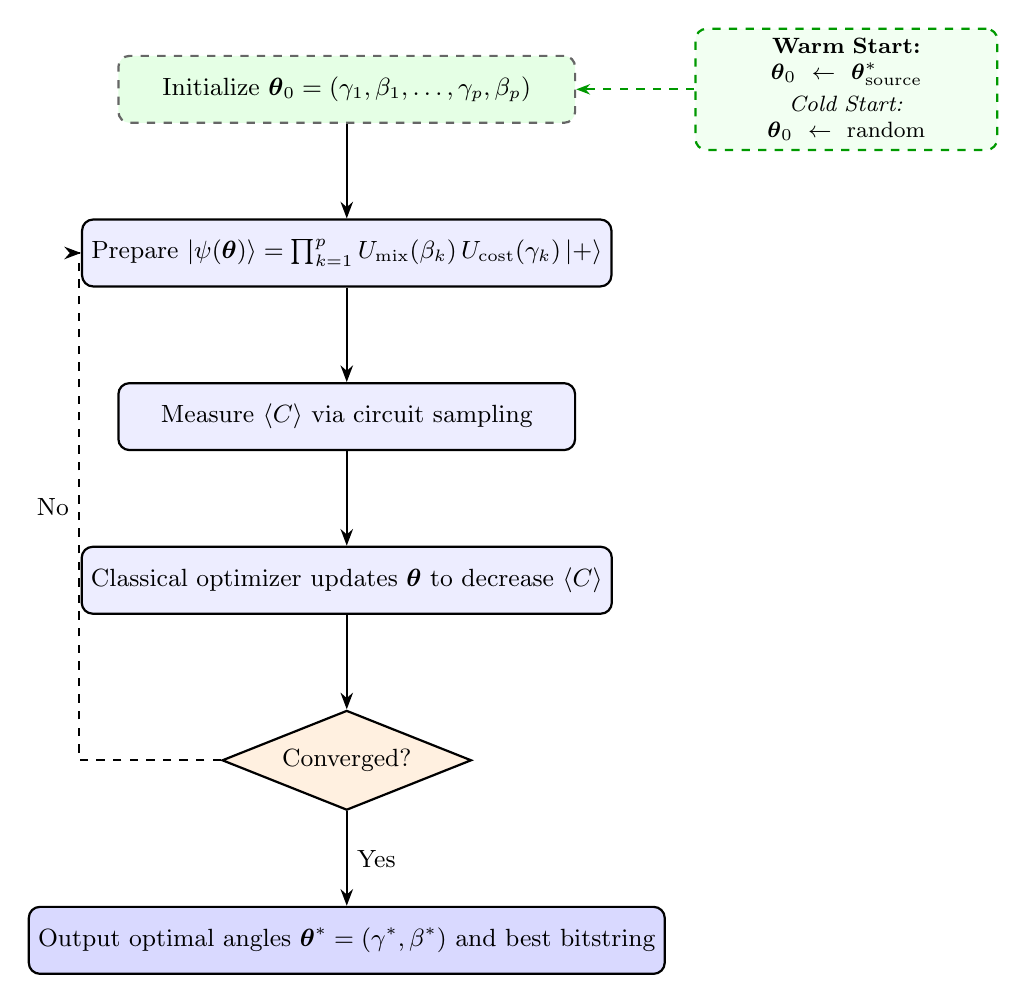
\begin{tikzpicture}[
    node distance=1.2cm and 2.5cm,
    every node/.style={font=\small},
    box/.style={
        rectangle, rounded corners=4pt,
        draw=black, thick,
        minimum width=5.8cm, minimum height=0.85cm,
        text centered, fill=blue!7
    },
    decision/.style={
        diamond, draw=black, thick,
        minimum width=2.8cm, minimum height=0.85cm,
        aspect=2.5, text centered, fill=orange!12
    },
    warmbox/.style={
        rectangle, rounded corners=4pt,
        draw=black!60, thick, dashed,
        minimum width=5.8cm, minimum height=0.85cm,
        text centered, fill=green!10
    },
    arrow/.style={-{Stealth[length=6pt]}, thick},
    backarrow/.style={-{Stealth[length=6pt]}, thick, dashed}
]

%% Nodes
\node[warmbox] (init) 
    {Initialize $\boldsymbol{\theta}_0 = (\gamma_1,\beta_1,\ldots,\gamma_p,\beta_p)$};

\node[box, below=of init] (state) 
    {Prepare $|\psi(\boldsymbol{\theta})\rangle = \prod_{k=1}^{p} U_\text{mix}(\beta_k)\,U_\text{cost}(\gamma_k)\,|{+}\rangle$};

\node[box, below=of state] (measure) 
    {Measure $\langle C \rangle$ via circuit sampling};

\node[box, below=of measure] (update) 
    {Classical optimizer updates $\boldsymbol{\theta}$ to decrease $\langle C \rangle$};

\node[decision, below=of update] (converge) 
    {Converged?};

\node[box, below=of converge, fill=blue!15] (done) 
    {Output optimal angles $\boldsymbol{\theta}^* = (\gamma^*,\beta^*)$ and best bitstring};

%% Warm-start annotation box
\node[
    draw=green!60!black, dashed, thick,
    rounded corners=4pt,
    fill=green!5,
    right=1.5cm of init,
    text width=3.6cm,
    align=center,
    font=\footnotesize
] (ws) 
    {\textbf{Warm Start:}\\
     $\boldsymbol{\theta}_0 \leftarrow \boldsymbol{\theta}^*_\text{source}$\\[2pt]
     \textit{Cold Start:}\\
     $\boldsymbol{\theta}_0 \leftarrow \text{random}$};

%% Main flow arrows
\draw[arrow] (init)     -- (state);
\draw[arrow] (state)    -- (measure);
\draw[arrow] (measure)  -- (update);
\draw[arrow] (update)   -- (converge);
\draw[arrow] (converge) -- node[right]{Yes} (done);

%% Loop-back arrow
\draw[backarrow] (converge.west)
    -- ++(-1.8,0)
    |- node[left, pos=0.25]{No} (state.west);

%% Warm-start annotation arrow
\draw[-{Stealth[length=5pt]}, green!60!black, thick, dashed]
    (ws.west) -- (init.east);

\end{tikzpicture}
\caption{QAOA variational optimization loop.}
\label{fig:qaoa-loop}
\end{figure}

The dashed green box highlights the initialization step where warm start replaces random cold-start initialization, reducing optimizer iterations and avoiding barren plateau regions.

The reason warm-start is so effective is the concentration phenomenon, which states that the optimal parameters for many combinatorial optimization problem classes concentrate around similar values across instances of the same size and structure \cite{warm-start}. Theoretical support for parameter reuse across instances was provided by Brandão et al., who proved that the QAOA objective landscape concentrates for typical instances drawn from random ensembles of instances\cite{fixedcontrolparametersquantum}, and empirically confirmed by Galda et al., who demonstrated transferability of optimal angles between structurally similar random graphs\cite{angletransfer}. 

The implementation follows three sequential phases. In the first phase, every sub-instance is solved independently using randomly initialized parameters to establish a baseline cost and produce an optimized parameter vector for each instance that serves as the transfer source for the next phases.

In the second phase, the optimized parameters from a source instance are passed directly as the initial point to the optimizer running on a different target instance of the same problem size. The optimizer continues to run to convergence from this starting point, so the quantum circuit still executes fully; the only difference from cold-start is where the search begins.

In the third phase, the optimized parameters are applied to a target instance with zero optimizer iterations. The parameters are fixed, the circuit is sampled directly, and the resulting bitstring distribution is decoded to extract the best valid tour. 

This is the strongest form of transfer: no quantum optimization is performed on the target at all. If this zero-shot application consistently recovers a near-optimal solution across diverse sub-instances, the result is consistent with the existence of a universal parameter vector for that problem size and structure class, allowing the solver to reuse it.

\section{Application Design and System Topology}
\label{sec:application-design}

To bridge the gap between abstract quantum computation and physical logistics, the platform relies on a highly normalized relational database and a bifurcated application pipeline. The Application Layer is divided into two primary environments: a monolithic web dashboard for administrative macro-dispatching, and a decoupled mobile edge node for driver micro-execution and telemetry generation.

\subsection{Interface Architecture and User Experience}
\label{sec:app-ux}

In high-throughput logistics, interface design is fundamentally an exercise in cognitive load management. The platform relies on processing massive arrays of complex spatial data; therefore, the user interfaces must distill this complexity into immediately actionable insights. The architecture eschews pervasive, trend-driven aesthetics in favor of a highly functional, minimalist paradigm termed ``Quiet Luxury.''

\subsubsection{Visual Identity and Typography}
The overarching visual identity prioritizes structural clarity and typographic hierarchy over decorative elements. 
\begin{itemize}
    \item \textbf{Monochromatic Depth:} The platform utilizes a strictly monochromatic base palette (slate and charcoal scales) to define container depths and structural boundaries. Semantic colors (success greens, error reds) are deployed sparingly and exclusively to indicate state changes or active telemetry.
    \item \textbf{Typographic Precision:} Adhering to editorial design principles, the application employs a highly legible sans-serif typeface. Data-dense tables and telemetry outputs utilize tabular lining figures to ensure strict vertical alignment of changing numerical data.
    \item \textbf{Unstyled Primitives:} To enforce this aesthetic programmatically, the dashboard utilizes Radix UI and Headless UI components. By relying on unstyled accessibility primitives rather than opinionated component libraries, the system maintains absolute control over visual weight via Tailwind CSS utility classes.
\end{itemize}

\subsubsection{Administrative Web Dashboard (React \& Inertia.js)}
The web application functions as the central command hub. To eliminate the overhead of managing a disparate REST API exclusively for the web frontend, the architecture utilizes the Inertia.js framework. This allows the frontend to operate as a modern Single-Page Application (SPA) using React, while natively inheriting Laravel's server-side routing, state, and security mechanisms.

Data visualizations and fleet routing geometries are managed through deep component decoupling. For example, the \texttt{OptimizeController} delegates the rendering of the fleet morphology to an isolated Mapbox GL component. Client-side state transitions such as toggling the visibility of specific driver geometries are managed entirely within the React DOM via \texttt{Zustand}, preventing redundant API calls and ensuring 60fps rendering fluidity.

\subsubsection{Driver-Facing Mobile Edge Node (Flutter)}
While the web dashboard is designed for data density, the Flutter mobile application is designed for environmental hostility. Drivers operate in fluctuating lighting conditions with high cognitive distractions; therefore, the mobile UX is strictly utilitarian.

\begin{itemize}
    \item \textbf{Environmental Adaptability:} The application defaults to a high-contrast, dark-mode paradigm, reducing screen glare and minimizing battery consumption on OLED displays—a critical constraint for devices running continuous GPS isolates.
    \item \textbf{Distraction-Free Execution:} The active navigation view eliminates macroscopic routing data, presenting the driver only with the immediate terminal node, the calculated trajectory, and an oversized, thumb-optimized call-to-action (CTA) for status updates.
    \item \textbf{Fluid Transitions:} To mask network latency when posting delivery photos or retrieving new payloads, the architecture employs GPU-accelerated micro-interactions, providing immediate tactile feedback to satisfy ISO/IEC 25010 operability standards.
\end{itemize}

\subsection{System Topology and Schema Architecture}
\label{sec:schema-architecture}

The relational database is architected to isolate identity management, macro-orchestration, and high-frequency edge telemetry. The schema is intrinsically \textbf{assignment-centric}, with the \texttt{driver\_assignments} table acting as the operational nexus that links the quantum solver's output to physical execution. Table \ref{tab:erd_mapping} details the core operational domains.

\begin{table}[htpb]
\centering
\caption{Core Entity-Relationship Mapping across the Logistics Platform}
\label{tab:erd_mapping}
\resizebox{\textwidth}{!}{
\begin{tabular}{llp{8cm}}
\toprule
\textbf{Domain} & \textbf{Primary Tables} & \textbf{Architectural Role \& Relationships} \\ 
\midrule
\textbf{Identity \& Auth} & \texttt{users}, \texttt{roles}, \texttt{permissions} & Base identity enriched with RBAC (Spatie), WebAuthn (Passkey) credentials, and 2FA states. API access is brokered via \texttt{personal\_access\_tokens} (Sanctum). \\
\midrule
\textbf{Orchestration} & \texttt{jobs}, \texttt{optimization\_histories} & Manages asynchronous QAOA computations. Histories maintain an audit log of solver parameters, elapsed execution time, and mathematical fairness gaps. \\
\midrule
\textbf{Route Assignment} & \texttt{dispatch\_routes}, \texttt{driver\_assignments} & \texttt{dispatch\_routes} act as named logical groupings. \texttt{driver\_assignments} contain the physical workload, linking drivers to serialized \texttt{geometry} and array-based completion statuses. \\
\midrule
\textbf{Telemetry \& Edge} & \texttt{driver\_locations}, \texttt{delivery\_photos} & Ingests high-frequency GPS pings mapped to active assignments. Photos enforce spatial verification by cross-referencing camera GPS stamps against intended stop coordinates. \\
\midrule
\textbf{Communications} & \texttt{messages}, \texttt{notifications} & Handles bi-directional chat, read receipts, and push-delivery tracking via mobile push tokens (FCM). \\
\bottomrule
\end{tabular}
}
\end{table}

Notably, the architecture intentionally decouples the overarching route identity (\texttt{dispatch\_routes}) from the physical vehicle allocations (\texttt{driver\_assignments}). This allows the system to requeue failed stops or reallocate specific geometric clusters dynamically without destroying the integrity of the original quantum solver output.

\subsubsection{Data Dictionary Definitions}
To ensure seamless serialization between the Python engine, the Laravel API, and the Dart edge node, the assignment and optimization payloads strictly adhere to the constraints defined in Table \ref{tab:schema_assignments} and Table \ref{tab:schema_optimization}.

\begin{table}[htpb]
\centering
\caption{Data Dictionary: \texttt{driver\_assignments} (Core Edge Workload)}
\label{tab:schema_assignments}
\resizebox{\textwidth}{!}{
\begin{tabular}{llll}
\toprule
\textbf{Attribute} & \textbf{Data Type} & \textbf{Constraints} & \textbf{Description} \\ 
\midrule
\texttt{id} & \texttt{UUID} & Primary Key & Unique identifier for the assignment fragment. \\
\texttt{driver\_id} & \textbf{\texttt{Foreign Key}} & Indexed, Nullable & Maps to \texttt{users.id}. Null if unassigned. \\
\texttt{instance} & \texttt{String} & Indexed & Links to the overarching \texttt{dispatch\_routes.name}. \\
\texttt{algorithm} & \texttt{String} & Not Null & Identifies the solver used (e.g., 'Recursive QAOA'). \\
\texttt{geometry} & \texttt{JSONB} & Not Null & Serialized GeoJSON array for Mapbox polyline rendering. \\
\texttt{stops} & \texttt{JSONB} & Not Null & Array of geographic coordinates representing the itinerary. \\
\texttt{stop\_statuses} & \texttt{JSONB} & Not Null & Mutating array tracking individual node completion states. \\
\texttt{status} & \texttt{Enum} & Default: 'pending' & State tracking: pending, dispatched, in\_transit, completed. \\
\bottomrule
\end{tabular}
}
\end{table}

\begin{table}[htpb]
\centering
\caption{Data Dictionary: \texttt{optimization\_histories} (Quantum Audit Log)}
\label{tab:schema_optimization}
\resizebox{\textwidth}{!}{
\begin{tabular}{llll}
\toprule
\textbf{Attribute} & \textbf{Data Type} & \textbf{Constraints} & \textbf{Description} \\ 
\midrule
\texttt{id} & \texttt{UUID} & Primary Key & Unique identifier for the solver execution instance. \\
\texttt{user\_id} & \textbf{\texttt{Foreign Key}} & Indexed & The dispatcher who initiated the quantum payload. \\
\texttt{k} & \texttt{Integer} & $k \ge 1$ & The exact vehicle fleet constraint applied to the solver. \\
\texttt{total\_distance} & \texttt{Decimal} & Not Null & The aggregate physical distance of the decoded routes. \\
\texttt{distance\_std} & \texttt{Decimal} & Not Null & The standard deviation ($\Sigma$) of workload distribution. \\
\texttt{elapsed} & \texttt{Decimal} & Not Null & Wall-clock execution time, crucial for cloud queue tracking. \\
\texttt{result} & \texttt{JSONB} & Not Null & The raw output array containing the mapped coordinate clusters. \\
\bottomrule
\end{tabular}
}
\end{table}

\subsection{Operational State Machines and Lifecycle Management}
\label{sec:operational-lifecycles}

The pipeline dictates how data flows from classical-quantum ingestion to physical execution. The system defines two concurrent, synchronized state machines: the Dispatcher Web Flow and the Driver Mobile Flow.

\subsubsection{Administrative Orchestration (React Monolith)}
The dispatcher interface is routed entirely through a secure web shell. As modeled in the overarching sequence diagram (Figure \ref{fig:uml_sequence}), the pipeline progresses from macro-planning to micro-oversight:
\begin{enumerate}
    \item \textbf{Ingestion \& Optimization:} Operating via the \texttt{OptimizeController}, the dispatcher selects a dataset, defines constraints, and executes the solver. The background Laravel queue processes the \texttt{Qiskit} job while the React frontend polls for completion via asynchronous HTTP 202 requests.
    \item \textbf{Dispatching:} The \texttt{DriverAssignmentController} fractures the finalized QUBO output into discrete driver itineraries, generating the \texttt{geometry} payloads and linking them to a \texttt{DispatchRoute} record.
    \item \textbf{Active Operations:} The \texttt{OperationsController} dashboard continuously ingests data from the \texttt{driver\_locations} table, rendering live fleet markers and detecting operational anomalies (e.g., stuck drivers).
\end{enumerate}

\begin{figure}[H]
    \centering
    % Replace 'Images/web_dashboard.png' with your actual file path
    \includegraphics[width=0.9\textwidth,height=0.90\textheight, keepaspectratio]{Images/web_dashboard.png}
    \caption{The React-based administrative dashboard, illustrating the live fleet map and tabular route telemetry.}
    \label{fig:web_dashboard}
\end{figure}

\clearpage
\begin{figure}[htpb]
    \centering
    % INSERT: Sequence Diagram Image Here
    \includegraphics[width=\textwidth, keepaspectratio]{Images/Chapter 3/uml_sequence.png}
    \caption{UML Sequence Diagram detailing the asynchronous quantum optimization and edge dispatch flow.}
    \label{fig:uml_sequence}
\end{figure}
\clearpage
\subsubsection{Edge Execution (Flutter Mobile Node)}
The driver application operates strictly via stateful REST API consumption, driven by native authentication and routing services.
\begin{enumerate}
    \item \textbf{Secure Initialization:} The driver authenticates via \texttt{/api/driver/login}. The device securely stores the Sanctum bearer token, registers an FCM token for push notifications, and triggers the \texttt{users} table presence tracking.
    \item \textbf{Workload Retrieval:} The application queries the \texttt{/api/driver/assignments} endpoint. The backend strictly scopes the response, delivering only the localized JSON payload assigned to that specific \texttt{driver\_id}.
    \item \textbf{Telemetry Loop:} A background isolate silently posts GPS coordinates to the \texttt{driver\_locations} table.
    \item \textbf{Proof of Delivery:} Upon reaching a node, the app updates the assignment's \texttt{stop\_statuses} and uploads environmental evidence (photos/signatures) to the \texttt{delivery\_photos} table, appending immediate GPS stamps for strict spatial compliance.
    \end{enumerate}
\begin{figure}[htpb]
    \centering
    % Screen 1
    \begin{subfigure}[b]{0.24\textwidth}
        \centering
        \includegraphics[width=\textwidth]{Images/Chapter 3/IMG_1772.PNG}
        \caption{Driver Dashboard}
        \label{fig:mobile_overview}
    \end{subfigure}
    \hfill
    % Screen 2
    \begin{subfigure}[b]{0.24\textwidth}
        \centering
        \includegraphics[width=\textwidth]{Images/Chapter 3/IMG_1773.PNG}
        \caption{Route Overview Page}
        \label{fig:mobile_nav}
    \end{subfigure}
    \hfill
    % Screen 3
    \begin{subfigure}[b]{0.24\textwidth}
        \centering
        \includegraphics[width=\textwidth]{Images/Chapter 3/IMG_1774.PNG}
        \caption{Single route map}
        \label{fig:mobile_camera}
    \end{subfigure}
    \hfill
    % Screen 4
    \begin{subfigure}[b]{0.24\textwidth}
        \centering
        \includegraphics[width=\textwidth]{Images/Chapter 3/IMG_1775.png}
        \caption{Delivery Confirmation}
        \label{fig:mobile_signature}
    \end{subfigure}
    
    \caption{The Flutter mobile application interface, demonstrating the strictly utilitarian, dark-mode execution environment utilized by the delivery fleet for telemetry and proof-of-delivery (POD) capture.}
    \label{fig:mobile_interfaces}
\end{figure}


\clearpage

\begin{figure}[htpb]
    \centering
    % INSERT: State Machine Diagram Image Here
    \includegraphics[width=0.85\textwidth,height=0.9\textheight, keepaspectratio]{Images/Chapter 3/uml_state.png}
    \caption{UML State Machine Diagram outlining the physical execution lifecycle of a driver assignment.}
    \label{fig:uml_state}
\end{figure}
\clearpage
To govern the physical reality of logistics, the \texttt{driver\_assignments} adhere to a strict state machine (Figure \ref{fig:uml_state}). The state progresses linearly from \texttt{Pending} to \texttt{Dispatched}. The \texttt{In\_Transit} state is dynamically triggered immediately upon ingesting the first GPS telemetry ping. Terminal states (\texttt{Completed} or \texttt{Failed}) are strictly gated; for an assignment to be marked as \texttt{Completed}, the system enforces that spatial verification constraints (valid \texttt{delivery\_photos} with correlating GPS stamps) must be met for every node in the localized cluster.





% Present the design developed.  (Please show your thought process given the requirements, constraints, and engineering standards.
% \begin{itemize}
%     \item Flow charts
%     \item Schematic 
%     \item Pseudo codes 
%     \item System-level diagrams
%     \item Architecture diagrams
%     \item System/transistor diagram
% \end{itemize}
% As shown in Figure \ref{fig:BlockDiag} below.

% \begin{figure}[ht]
%     \centering
%     \includegraphics[scale=1]{Images/block1.png}
%     \caption{Main System Design}
%     \label{fig:BlockDiag}
% \end{figure}


% This section should also discuss how the proposed design will satisfy each requirement, given the realistic constraints of the design problem. See Figure \ref{fig:SubSystem} .


% \begin{figure}[ht]
%     \centering
%     \includegraphics[scale=0.6]{Images/sub_sys.png}
%     \caption{Sub System Design}
%     \label{fig:SubSystem}
% \end{figure}

\chapter{Results}

\section{Setup}
\subsection{Environment Setup}

All project dependencies were isolated within a dedicated Python virtual
environment managed via \texttt{conda}. The environment runs Python~3.12.12,
with all packages installed through \texttt{pip}, and was initialised using:

\begin{verbatim}
conda create -n quantum-solver python=3.12.12
conda activate quantum-solver
\end{verbatim}

\subsubsection{Core Quantum Dependencies}

The quantum components of the solver depend on four Qiskit packages. These
must be installed in the exact versions shown below to ensure
compatibility:

\begin{verbatim}
pip install qiskit==1.4.2           \
            qiskit-aer==0.17.0      \
            qiskit-algorithms==0.3.1 \
            qiskit-optimization==0.6.1
\end{verbatim}

Each package provides the following functionality:

\begin{itemize}
    \item \textbf{qiskit}: Quantum circuit construction, transpilation, and
          QAOA ansatz generation.
    \item \textbf{qiskit-aer}: High-performance statevector simulator backend.
    \item \textbf{qiskit-algorithms}: Variational optimisers, including
          COBYLA, ADAM, and SPSA.
    \item \textbf{qiskit-optimization}: The \texttt{QuadraticProgram}
          interface and QUBO conversion utilities.
\end{itemize}

\subsubsection{Classical and Utility Libraries}

The following packages cover the classical baseline solvers and general
numerical and visualisation utilities:

\begin{verbatim}
pip install ortools numpy matplotlib
\end{verbatim}

Google OR-Tools provides the classical baseline; NumPy handles all numerical
computation; Matplotlib produces route visualisations and plots.

\subsubsection{IBM Quantum Hardware Libraries}

Executing circuits on real IBM Quantum hardware requires additional libraries
and credentials beyond the standard simulation setup. These were used to
validate hardware compatibility on a small 5-node instance via an IBM Cloud
account, through a dedicated service instance
identified by its Cloud Resource Name (CRN).

Install the required IBM Quantum runtime libraries as follows:

\begin{verbatim}
pip install qiskit-ibm-runtime
pip install qiskit-ibm-provider
\end{verbatim}

\begin{itemize}
    \item \textbf{qiskit-ibm-runtime}: The primary interface for submitting
          jobs to IBM Quantum hardware. It provides the
          \texttt{QiskitRuntimeService} class for authentication, backend
          selection, and job management, and exposes IBM's \texttt{Sampler}
          and \texttt{Estimator} primitives.

    \item \textbf{qiskit-ibm-provider}: A lower-level provider package that
          grants direct access to IBM Quantum backends, enabling users to list
          available devices, inspect their properties (qubit count,
          connectivity, error rates, and queue depth), and submit circuits
          directly to a chosen backend.
\end{itemize}

Running circuits on IBM Quantum hardware has the following prerequisites:

\begin{itemize}
    \item \textbf{IBM Cloud Account}: An active IBM Cloud account.

    \item \textbf{Quantum Service Instance}: A Quantum Computing service
          instance identified by its CRN. To obtain one,the instance tab must be navigated to  on the IBM Quantum Platform,  a new instance must be created,
          and its CRN must be copied, as shown in Figure~\ref{fig:ibm-crn}.

    \begin{figure}[h]
        \centering
        \includegraphics[width=\linewidth]{Images/chapter4/ibm crn.png}
        \caption{Locating the CRN for an IBM Quantum service instance.}
        \label{fig:ibm-crn}
    \end{figure}

    \item \textbf{API Token}: An API token generated from the IBM Quantum
          Platform, which links the local environment to the IBM Cloud account
          and its associated service instance. The token can be generated by
          navigating to the Home tab and selecting \emph{Create an API key},
          as shown in Figure~\ref{fig:ibm-api}.

    \begin{figure}[h]
        \centering
        \includegraphics[width=\linewidth]{Images/chapter4/ibm api.png}
        \caption{Generating an API token on the IBM Quantum Platform.}
        \label{fig:ibm-api}
    \end{figure}
\end{itemize}

Once the prerequisites are satisfied, hardware access can be authenticated
and a backend selected as follows:

\begin{verbatim}
from qiskit_ibm_runtime import QiskitRuntimeService

QiskitRuntimeService.save_account(
    channel="ibm_cloud",
    token="API-TOKEN",
    instance="CRN",
)

service = QiskitRuntimeService()
backend = service.backend("target_backend_name")
\end{verbatim}

The target backend should be selected based on qubit count, error rates, and
current queue depth, all of which are accessible through the IBM Quantum
Platform dashboard.
\subsubsection{System Dependencies and Ecosystem Support}

To satisfy the manufacturability and sustainability constraints defined in Chapter 1, the hybrid routing platform eschews proprietary, monolithic software suites in favor of highly modular, community-supported open-source ecosystems. The architecture relies on the Laravel (PHP 8.3+) and React (Node.js) environments, bridged seamlessly via Inertia.js. This eliminates the overhead of managing a disparate REST API for the administrative dashboard, allowing the frontend to operate as a single-page application (SPA) while natively inheriting Laravel's server-side routing and state.

Table \ref{tab:system_dependencies} outlines the primary functional dependencies utilized to construct the production environment. These packages were selected based on their active maintenance lifecycles, strict type-safety (TypeScript/PHPStan), and adherence to enterprise security standards.

\begin{table}[htpb]
\centering
\caption{Core Functional Dependencies across the Hybrid Architecture}
\label{tab:system_dependencies}
\resizebox{\textwidth}{!}{
\begin{tabular}{lll}
\toprule
\textbf{Category} & \textbf{Core Technologies} & \textbf{Implementation Purpose} \\ 
\midrule
\textbf{Application Bridge} & Inertia.js, Vite & Seamless SPA state management and asset compilation. \\
\textbf{Spatial \& Data Viz.} & Mapbox GL, TopoJSON, Recharts, OSMNX & High-fidelity route rendering and metrics visualization. \\
\textbf{UI Architecture} & Radix UI, Headless UI, Tailwind CSS & Unstyled, accessible primitives for a bespoke, minimalist interface. \\
\textbf{Motion \& Fluidity} & Framer Motion, tw-animate-css & GPU-accelerated transitions for dynamic dashboard updates. \\
\midrule
\textbf{Security \& Auth} & Laravel Sanctum, Fortify & Stateless API authentication and secure session scaffolding. \\
\textbf{Advanced Identity} & WebAuthn, Google2FA & Biometric (Passkey) and two-factor authentication integration. \\
\textbf{System Orchestration} & Laravel Queues, Cron Expression & Asynchronous handling of long-running QAOA quantum jobs. \\
\midrule
\textbf{Testing \& QA} & Pest PHP, ParaTest & Parallelized unit and feature testing with strict coverage thresholds. \\
\textbf{Static Analysis} & PHPStan, Architecture Test & Automated enforcement of architectural boundaries and side-effect detection. \\
\bottomrule
\end{tabular}
}
\end{table}

\vspace{1em}
\noindent\textbf{Security and GRC Compliance Integration}

The backend ecosystem specifically supports the Governance, Risk, and Compliance (GRC) objectives of the logistics platform. By utilizing packages such as \texttt{laragear/webauthn} and \texttt{pragmarx/google2fa}, the system is equipped to handle biometric passkeys and multi-factor authentication. This ensures that the dispatching of quantum-optimized routes is restricted strictly to authorized fleet administrators, fulfilling the role-based access constraints required for secure enterprise deployments.

Furthermore, the integration of \texttt{pestphp/pest} alongside architectural testing libraries guarantees that the complex business logic bridging the classical algorithms and the Qiskit execution layer remains functionally isolated and mathematically verifiable across deployment iterations.

\subsection{Problem Instance}

The test instances used across all experiments are drawn from a real-world
benchmark suite. Each instance was generated using:

\begin{verbatim}
java -jar Benchmark.jar
\end{verbatim}



After launching the tool, the desired instance number is entered,
and a \texttt{.vrp} file is produced for that instance. This process was
repeated for all instances used in this work.


\section{Testing }
Given the hybrid nature of the architecture, the testing protocol was divided into three distinct phases: algorithmic validation of the quantum solver, integration testing of the inter-service bridge, and end-to-end evaluation of the administrative and driver interfaces. This multi-tiered approach ensures that both the mathematical integrity of the QUBO formulations and the operational stability of the logistics platform meet the ISO/IEC 25010 reliability standards outlined in Chapter 1.

\subsection{Algorithmic and Quantum Layer Testing (Python \& Qiskit)}

The core optimization engine was subjected to rigorous unit and stress testing to validate the classical decomposition and quantum execution logic.

\begin{itemize}
    \item \textbf{Deterministic Seeding and Reproducibility:} To ensure testing consistency across stochastic algorithms, all Python testing suites were initialized with fixed random seeds during development. This allowed for precise regression testing.
    \item \textbf{Statevector Threshold Validation:} The recursive clustering logic was stress-tested to guarantee that no leaf sub-problem exceeded the 29-qubit limit of the Qiskit Aer statevector simulator. Instances of up to 1,000 nodes were fed into the pipeline specifically to verify that the $n \le 5$ constraint remained absolute and prevented memory overflow errors.
    \item \textbf{Subtour Elimination Verification:} The edge-based QUBO formulations for $k > 1$ scenarios generate solutions that must be checked for disconnected cycles. The decoding logic was rigorously tested against edge-case bitstrings to ensure that the post-hoc subtour filtering accurately rejected invalid graphs before they could be passed to the classical stitching layer.
\end{itemize}

\subsection{Integration and Orchestration Testing (Laravel \& Python Bridge)}

Because quantum circuit execution introduces significant and variable latency, testing the communication between the Laravel backend and the Python microservice was a critical priority.

\begin{itemize}
    \item \textbf{Asynchronous Queue Stability:} Laravel's queue worker system was tested under heavy load to ensure that long-running QAOA jobs (such as the 921-second execution for the 1,000-node instance) did not trigger standard HTTP timeouts. Jobs were actively monitored to verify that their states transitioned correctly from "Pending" to "Processing" and "Completed."
    \item \textbf{Fallback Mechanisms:} The API bridge was subjected to simulated failures such as: disconnecting the Python service or simulating a QPU queue timeout. The system was validated to ensure it gracefully engaged the classical fallback mechanisms without crashing the end-user application or dropping the delivery payload.
\end{itemize}



\subsection{End-to-End System Testing (React \& Flutter)}

The final testing phase focused on the client-side applications, ensuring the complex spatial data generated by the solver translated seamlessly into actionable logistics operations.

\begin{itemize}
    \item \textbf{State Management and Rendering:} The React administrative dashboard was stress-tested by injecting the massive 1,000-node solution data. The \texttt{Zustand} state manager and Mapbox/React-Map-GL components were evaluated for frame drops, ensuring that the dispatcher interface maintained fluid 60fps rendering even when rendering hundreds of intersecting polylines.
    \item \textbf{Role-Based Access Control (RBAC):} Secure authentication flows were tested to ensure strict boundaries between roles. Tests verified that dispatchers could view all active nodes and approve solver runs, while driver accounts on the Flutter application were strictly limited to receiving and interacting with their explicitly assigned route arrays.
    \item \textbf{Cross-Platform UI Fidelity:} The Flutter driver application was deployed to both iOS and Android simulators to verify that the customized "Quiet Luxury" typographic and layout standards rendered consistently across different screen aspect ratios and pixel densities.
\end{itemize}
\section{Results Discussion }\subsection{Hyper-Parameter Sweep Results}
\label{sec:hyperparameter-results}

A total of 1,728 quantum circuits were evaluated using three dataset instances and 
576 combinations of classical optimizer, number of layers ($p$), penalty, number 
of vehicles ($k$), maximum iterations (\texttt{maxiter}), and restarts. Two 
criteria were used for evaluation: the failure rate, defined as the proportion of 
runs in which no valid solution was found, and the rank-1 rate, defined as the 
proportion of runs in which the optimal solution was assigned the highest 
probability by the circuit.

As shown in the tables below, all three optimizers achieved comparable rank-1 
rates, indicating that when a valid solution is found, all three locate the optimum 
at similar frequencies. The key distinction lies in the failure rate. ADAM's 
elevated failure rate is consistent with its adaptive learning rate overshooting 
in the characteristically flat QAOA energy landscape at small leaf sizes, causing 
the optimizer to diverge rather than converge to a feasible solution. COBYLA was 
therefore selected as the optimizer for the final design.

\begin{table}[htbp]
    \centering
    \resizebox{\textwidth}{!}{%
    \begin{tabular}{l c c c c c}
    \hline
    \textbf{Optimizer} & \textbf{Total Runs} & \textbf{Failures} & 
    \textbf{Failure Rate (\%)} & \textbf{Rank-1 Count} & \textbf{Rank-1 Rate (\%)} \\
    \hline
    ADAM   & 576 & 232 & 40.28 & 188 & 32.64 \\
    COBYLA & 576 & 36  & 6.25  & 177 & 30.73 \\
    SPSA   & 576 & 169 & 29.34 & 174 & 30.21 \\
    \hline
    \end{tabular}%
    }
    \caption{Failure and Rank-1 Rates by Optimizer}
    \label{tab:optimizer_rates}
\end{table}

The number of restarts controls how many times the optimizer is re-initialized 
from a different starting point, reducing the likelihood of convergence to a local 
minimum. As shown below, increasing restarts from 1 to 3 reduced the failure rate 
by 15.16\% and improved the rank-1 rate by 7.76\%. A restart value of 3 was 
therefore adopted.

\begin{table}[!ht]
\centering
\begin{tabular}{@{}lllll@{}}
\toprule
\textbf{Restarts} & \textbf{Total Runs} & \textbf{Failures} & 
\textbf{Failure Rate (\%)} & \textbf{Rank-1 Rate (\%)} \\ \midrule
1 & 864 & 284 & 32.87 & 27.31 \\
3 & 864 & 153 & 17.71 & 35.07 \\ \bottomrule
\end{tabular}
\caption{Failure Rate and Rank-1 Rate by Restarts}
\label{tab:restarts-failure-rank}
\end{table}

The effect of \texttt{maxiter} was found to be optimizer-dependent. For ADAM, 
increasing \texttt{maxiter} from 50 to 200 produced no change in either failure 
rate or rank-1 rate, confirming that ADAM converges well within the lower budget. 
COBYLA behaved similarly, with no change in failure rate and only a marginal 
1.04 percentage point reduction in rank-1 rate, indicating that COBYLA reaches 
its optimum rapidly and does not benefit from additional iterations. SPSA was the 
only optimizer to show a meaningful improvement, reducing its failure rate by 5.21 
percentage points at the higher budget. Since COBYLA was selected as the final 
optimizer, and given that it shows no sensitivity to \texttt{maxiter} beyond 50, 
a value of \texttt{maxiter} $= 50$ was adopted for all final configurations.

\begin{table}[!ht]
\centering
\begin{tabular}{@{}lllllll@{}}
\toprule
 & \multicolumn{3}{c}{\textbf{Failure Rate (\%)}} & 
   \multicolumn{3}{c}{\textbf{Rank-1 Rate (\%)}} \\ 
\cmidrule(lr){2-4} \cmidrule(lr){5-7}
\textbf{Optimizer} & \textbf{maxiter=50} & \textbf{maxiter=200} & 
$\boldsymbol{\Delta}$ & \textbf{maxiter=50} & \textbf{maxiter=200} & 
$\boldsymbol{\Delta}$ \\ \midrule
ADAM   & 40.28 & 40.28 & 0.00  & 32.64 & 32.64 & 0.00  \\
COBYLA & 6.25  & 6.25  & 0.00  & 31.25 & 30.21 & -1.04 \\
SPSA   & 31.94 & 26.74 & -5.21 & 30.56 & 29.86 & -0.69 \\ \bottomrule
\end{tabular}
\caption{Failure Rate and Rank-1 Rate (\%) by Optimizer and MaxIter}
\label{tab:optimizer-maxiter}
\end{table}

The number of QAOA layers $p$ directly controls circuit depth and approximation 
quality. Notably, COBYLA achieved a failure rate of 0.00\% at $p = 2$, which is 
the strongest result observed across all parameter combinations. A value of 
$p = 2$ was therefore selected, as it eliminates failures entirely for COBYLA 
while keeping circuit depth within the simulation constraints discussed earlier.

\begin{table}[!ht]
\centering
\resizebox{\textwidth}{!}{%
\begin{tabular}{@{}lrrrrrrrrrrr@{}}
\toprule
 & \multicolumn{5}{c}{\textbf{Failure Rate (\%)}} & 
   \multicolumn{5}{c}{\textbf{Rank-1 Rate (\%)}} \\ 
\cmidrule(lr){2-6} \cmidrule(lr){7-11}
\textbf{Optimizer} & \textbf{p=1} & \textbf{p=2} & \textbf{p=3} & \textbf{p=5} & 
\textbf{Row} & \textbf{p=1} & \textbf{p=2} & \textbf{p=3} & \textbf{p=5} & 
\textbf{Row} \\ \midrule
ADAM   & 61.11 & 23.61 & 43.06 & 33.33 & 40.28 & 15.28 & 37.50 & 41.67 & 36.11 & 32.64 \\
COBYLA & 1.39  & 0.00  & 15.28 & 8.33  & 6.25  & 27.78 & 29.17 & 30.56 & 35.42 & 30.73 \\
SPSA   & 25.00 & 29.17 & 30.56 & 32.64 & 29.34 & 36.11 & 22.92 & 31.94 & 29.86 & 30.21 \\ \midrule
\textbf{Col} & 29.17 & 17.59 & 29.63 & 24.77 & 25.29 & 26.39 & 29.86 & 34.72 & 33.80 & 31.19 \\ \bottomrule
\end{tabular}%
}
\caption{Failure Rate and Rank-1 Rate (\%) by Optimizer and Reps}
\label{tab:optimizer-reps}
\end{table}

\begin{figure}[!ht]
    \centering
    \includegraphics[width=0.8\linewidth]{Images/chapter4/Screenshot 2026-05-01 193349.png}
    \caption{Failure Rate by Optimizer and Reps}
    \label{fig:failure-rate-optimizer-reps}
\end{figure}

\begin{figure}[!ht]
    \centering
    \includegraphics[width=0.8\linewidth]{Images/chapter4/Screenshot 2026-05-01 193627.png}
    \caption{Rank-1 Rate by Optimizer and Reps}
    \label{fig:rank1-rate-optimizer-reps}
\end{figure}

The choice of QUBO formulation was found to have a significant effect on solution 
validity. The position-indexed formulation, which eliminates subtours structurally, 
achieved a failure rate of 8.56\%, compared to 30.86\% for the edge-based 
formulation. This is consistent with the theoretical expectation that structural 
constraint elimination reduces the burden on the classical optimizer and produces 
a more navigable energy landscape.

\begin{table}[!ht]
\centering
\begin{tabular}{@{}llll@{}}
\toprule
\textbf{Formulation} & \textbf{Total Runs} & \textbf{Failures} & 
\textbf{Failure Rate (\%)} \\ \midrule
Position-Indexed & 432  & 37  & 8.56  \\
Edge-Based       & 1296 & 400 & 30.86 \\ \bottomrule
\end{tabular}
\caption{Failure Rate by QUBO Formulation}
\label{tab:qubo-formulation}
\end{table}

Three penalty multiplier values were evaluated. A penalty of 2 produced both the 
lowest failure rate (24.48\%) and the highest rank-1 rate (35.24\%), outperforming 
penalties of 5 and 10 on both metrics. The failure rates across all three values 
were sufficiently close that the rank-1 rate was the deciding factor. A penalty 
multiplier of 2 was therefore adopted.

\begin{table}[!ht]
\centering
\begin{tabular}{@{}rrrrr@{}}
\toprule
\textbf{Penalty Mult} & \textbf{Total Runs} & \textbf{Failures} & 
\textbf{Failure Rate (\%)} & \textbf{Rank-1 Rate (\%)} \\ \midrule
2  & 576 & 141 & 24.48 & 35.24 \\
5  & 576 & 149 & 25.87 & 27.60 \\
10 & 576 & 147 & 25.52 & 30.73 \\ \bottomrule
\end{tabular}
\caption{Failure Rate and Rank-1 Rate by Penalty Multiplier}
\label{tab:penalty-failure-rank}
\end{table}

The runtime analysis confirmed that SPSA, averaging 156.31s per run, is 
impractical. ADAM averaged 8.52s, but at the cost of the highest failure rate. 
COBYLA averaged 27.70s, a trade-off consistent with quantum optimization 
literature, as derivative-free methods require more function evaluations per run 
but produce significantly more reliable solutions. Runtime scaled predictably with 
both $p$ and restarts, as shown below. The selected configuration of COBYLA, 
$p = 2$, \texttt{maxiter} $= 50$, penalty $= 2$, and 3 restarts was therefore 
used for all subsequent experiments.

\begin{table}[!ht]
\centering
\begin{tabular}{@{}lll@{}}
\toprule
\textbf{Parameter} & \textbf{Value} & \textbf{Avg Time (s)} \\ \midrule
\multirow{3}{*}{Optimizer} & ADAM   & 8.52   \\
                           & COBYLA & 27.70  \\
                           & SPSA   & 156.31 \\ \midrule
\multirow{4}{*}{Reps ($p$)} & 1 & 41.64 \\
                             & 2 & 54.93 \\
                             & 3 & 66.04 \\
                             & 5 & 94.10 \\ \midrule
\multirow{2}{*}{Restarts}  & 1 & 32.29 \\
                           & 3 & 96.07 \\ \midrule
\multirow{2}{*}{MaxIter}   & 50  & 36.43 \\
                           & 200 & 91.93 \\ \bottomrule
\end{tabular}
\caption{Average Runtime by Hyperparameter}
\label{tab:avg-runtime}

\end{table}
\begin{figure}
    \centering
    \includegraphics[width=1\linewidth]{Images/chapter4/time.png}
    \caption{Average Time for Each Parameter}
    \label{fig:placeholder}
\end{figure}
\subsection{Cold-Start vs.\ Warm-Start QAOA Optimization}

The point of this experiment is to test whether QAOA $\gamma$ and $\beta$ parameters learned on a certain sub-instance of the VRP can serve as effective initializations for the optimization of structurally related sub-instances. Successful parameter transfer allows the solver to skip expensive re-optimization on each new sub-problem, which should also reduce the total quantum runtime by 80-90\% without affecting solution quality.

Seven QAOA configurations were evaluated under two initialization strategies across 18 TSP leaf instances covering 2, 3, and 4 customer sub-problems. The instances derived from the benchmark spanned different geometric configurations and clusters to test whether warm-start benefit is geometry-dependent. 
Tables \ref{tab:instances-4cust}, \ref{tab:instances-2cust} and \ref{tab:instances-3cust} show the geometry for different number of customers.

\begin{table}[h]
\centering
\begin{tabular}{cll}
\hline
\textbf{Label} & \textbf{Node IDs} & \textbf{Geometry} \\
\hline
A & 1, 2, 3, 4     & First four delivery nodes; original solver sub-route \\
B & 7, 14, 21, 35  & Sparse original sub-route \\
C & 8, 10, 29, 45  & Sparse original sub-route \\
D & 16, 23, 28, 38 & Compact center: spatially tight central cluster \\
E & 3, 15, 37, 42  & Compact east: tight cluster on the eastern side \\
F & 39, 40, 43, 47 & Compact northwest: tight cluster \\
G & 1, 10, 46, 47  & Spread corners: nodes near bounding-box extremes \\
H & 20, 13, 36, 40 & Spread diagonal: maximally distant diagonal pair \\
I & 17, 26, 31, 49 & Near-depot: small Euclidean distances to the depot \\
J & 9, 13, 24, 46  & Far-from-depot: large Euclidean distances to the depot \\
K & 17, 7, 44, 20  & Mixed: heterogeneous inter-node distances \\
L & 5, 41, 14, 22  & Mixed: one node sampled from each geographic quadrant \\
M & 2, 33, 36, 19  & Random spread: no deliberate geometric structure \\
\hline
\end{tabular}
\caption{4-Customer Sub-Instances (16 qubits, $n^2 = 4^2$)}
\label{tab:instances-4cust}
\end{table}

\begin{table}[h]
\centering
\begin{tabular}{cll}
\hline
\textbf{Label} & \textbf{Node IDs} & \textbf{Geometry} \\
\hline
S1 & 17, 26 & Near: short inter-node distance \\
S2 & 9, 46  & Far: large inter-node distance \\
S3 & 4, 11  & Mid: intermediate inter-node distance \\
\hline
\end{tabular}
\caption{2-Customer Sub-Instances (4 qubits, $n^2 = 2^2$)}
\label{tab:instances-2cust}
\end{table}

\begin{table}[h]
\centering
\begin{tabular}{cll}
\hline
\textbf{Label} & \textbf{Node IDs} & \textbf{Geometry} \\
\hline
T1 & 16, 23, 28 & Compact: spatially tight cluster (subset of instance D) \\
T2 & 1, 46, 20  & Spread: geographically dispersed nodes \\
T3 & 7, 36, 43  & Mixed: heterogeneous spatial configuration \\
\hline
\end{tabular}
\caption{3-Customer Sub-Instances (9 qubits, $n^2 = 3^2$)}
\label{tab:instances-3cust}
\end{table}

The experiment is split into 3 phases:
\begin{itemize}
    \item Phase 1: Cold-Start Baseline\newline
    Each of the 19 instances is solved independently using QAOA with parameters that are drawn at random every run. 5 optimizer configurations were tested per instance, adding up to 95 runs in total. The results establish a performance ceiling for each instance.
    \item Phase 2: Warm-Start Baseline\newline
    For each of the 36 pairs, the optimal parameters from the source instance obtained in Phase 1 are used as the initial parameters for the optimizer. 5 configurations are evaluated per pair, giving a total of 180 runs.
    \item Phase 3: Parameter Universality\newline
    The optimized parameters of each instance are directly applied to every same-size instance without any further optimization. The point is to test the existence of a universal $\gamma$ and $\beta$ that generalizes across instances of the same size and problem class.
\end{itemize}

Table 4.19 below shows the results when comparing Cold-Start with Warm-Start. 6 out of 7 configurations were already reaching 100\% optimality under cold-start with zero effect of warm-start on them, except for the  configuration \textit{p=2, COBYLA, maxiter=100, restarts=1}. This configuration struggled in cold-start due to it being a shallow circuit. The tight budget is not enough for cold-start to reliably find the optimum, but seeding from a geometrically similar instance brings it to the same starting region as a good solution, proving that warm-start has effectively rescued this case from failing and providing 100\% optimality.

\begin{table}[ht]
\centering
\setlength{\tabcolsep}{4pt}
\begin{tabular}{lcccc|cccc|c}
\toprule
\multirow{2}{*}{\textbf{Configuration}}
  & \multicolumn{4}{c|}{\textbf{Cold Start (Phase 1)}}
  & \multicolumn{4}{c|}{\textbf{Warm Start (Phase 2)}}
  & \multirow{2}{*}{\textbf{$\Delta$Gap}} \\
\cmidrule(lr){2-5}\cmidrule(lr){6-9}
  & OptRate & AvgGap & AvgTime & Fail
  & OptRate & AvgGap & AvgTime & Fail & \\
\midrule
$p{=}2$, ADAM,   mi$=30$, re$=1$ & 100.0\% & 0.00\% & 0.4\,s & 0
                                  & 100.0\% & 0.00\% & 0.4\,s & 0 & $+0.00$ \\
$p{=}5$, ADAM,   mi$=30$, re$=1$ & 100.0\% & 0.00\% & 1.0\,s & 0
                                  & 100.0\% & 0.00\% & 1.0\,s & 0 & $+0.00$ \\
$p{=}2$, COBYLA, mi$=100$, re$=1$ &  89.5\% & 0.62\% & 2.8\,s & 2
                                  & 100.0\% & 0.00\% & 2.6\,s & 0 & $\mathbf{-0.62}$ \\
$p{=}2$, ADAM,   mi$=80$,  re$=2$ & 100.0\% & 0.00\% & 0.7\,s & 0
                                  & 100.0\% & 0.00\% & 0.7\,s & 0 & $+0.00$ \\
$p{=}5$, COBYLA, mi$=100$, re$=1$ & 100.0\% & 0.00\% & 8.3\,s & 0
                                  & 100.0\% & 0.00\% & 7.4\,s & 0 & $+0.00$ \\
$p{=}2$, COBYLA, mi$=50$,  re$=3$ & 100.0\% & 0.00\% & 9.9\,s & 0
                                  & 100.0\% & 0.00\% & 7.5\,s & 0 & $+0.00$ \\
$p{=}5$, COBYLA, mi$=50$,  re$=3$ & 100.0\% & 0.00\% & 12.8\,s & 0
                                  & 100.0\% & 0.00\% & 11.8\,s & 0 & $+0.00$ \\
\bottomrule
\end{tabular}
\caption{Phase~1 vs.\ Phase~2: Cold-Start vs.\ Warm-Start Optimization.}
\label{tab:exp6_phase12}
\end{table}

Metrics are averaged over all instances possessing a warm-start pair. $\Delta$Gap $= $ Warm AvgGap $-$ Cold AvgGap; negative values indicate improvement from warm-starting.

Moreover, warm-start gave a humble wall-time reduction on restart-heavy or large \textit{maxiter} configurations, like the instance \textit{p=5, COBYLA, mi=100: 8.3s → 7.4s}, as COBYLA needs fewer iterations to converge when it starts closer to the optimum.

\subsubsection{Parameter Universality: Direct Transfer Without Re-Optimization}

Phase~3 tests whether optimal parameters found for one instance can be used directly in a different instance without any re-optimization. This probes the flatness and universality of the QAOA energy landscape. All ADAM-based configurations transfer perfectly across
all 3 qubit sizes achieving 100\% optimal rate and 0.00\% gap. This behavior stems from ADAM converging to a single dominant basin in the landscape, shared by all
instances of the same problem class. As shown in table \ref{tab:wsallphases}, COBYLA with a tight budget ($p{=}2$, maxiter$=100$, restarts$=1$) degrades at 16 qubits, yielding only 83\% optimal rate, and an infinite average gap due to infeasible bitstrings. This happens because COBYLA is a derivative-free optimizer that searches locally and starts from the nearest minimum. At 16 qubits, that landscape becomes complex enough that COBYLA's tight budget locks it into instance-specific local minima that happens to work for the instance it was trained on, but doesn't genaralize. On the other hand, ADAM uses a momentum-based gradient estimator that searches toward basins that are shared across instances of the same problem class.

\begin{table}[ht]
\centering
\setlength{\tabcolsep}{5pt}
\begin{tabular}{lcc|cc|cc}
\toprule
\multirow{2}{*}{\textbf{Configuration}}
  & \multicolumn{2}{c|}{\textbf{2-cust (4\,q)}}
  & \multicolumn{2}{c|}{\textbf{3-cust (9\,q)}}
  & \multicolumn{2}{c}{\textbf{4-cust (16\,q)}} \\
\cmidrule(lr){2-3}\cmidrule(lr){4-5}\cmidrule(lr){6-7}
  & OptR & AvgGap & OptR & AvgGap & OptR & AvgGap \\
\midrule
$p{=}2$, ADAM,   mi$=30$,  re$=1$ & 100\% & 0.00\% & 100\% & 0.00\% & 100\% & 0.00\% \\
$p{=}5$, ADAM,   mi$=30$,  re$=1$ & 100\% & 0.00\% & 100\% & 0.00\% & 100\% & 0.00\% \\
$p{=}2$, COBYLA, mi$=100$, re$=1$ & 100\% & 0.00\% & 100\% & 0.00\% &  83\% & $\infty$ \\
$p{=}2$, ADAM,   mi$=80$,  re$=2$ & 100\% & 0.00\% & 100\% & 0.00\% & 100\% & 0.00\% \\
$p{=}5$, COBYLA, mi$=100$, re$=1$ & 100\% & 0.00\% & 100\% & 0.00\% & 100\% & 0.00\% \\
$p{=}2$, COBYLA, mi$=50$,  re$=3$ & 100\% & 0.00\% & 100\% & 0.00\% & 100\% & 0.00\% \\
$p{=}5$, COBYLA, mi$=50$,  re$=3$ & 100\% & 0.00\% & 100\% & 0.00\% & 100\% & 0.00\% \\
\bottomrule
\end{tabular}
\caption{Phase~3: Parameter Universality via direct transfer.}
\label{tab:wsphase3}
\end{table}

OptR = optimal rate; AvgGap = mean optimality gap. ``$\infty$'' indicates at least one transfer produced an infeasible solution with unbounded gap.

\subsubsection{Warm-Start Value Across All Phases}

Synthesizing all three phases, warm-start provides a decisive benefit only for the budget-constrained COBYLA configuration \textit{$p{=}2$, maxiter$=100$,
restarts$=1$}, where it saves two cold-start failures and restores full optimality. For every other configuration, cold-start, warm-start, and
direct parameter transfer all converge to 100\% optimal, leaving warm-start with at most a wall-time advantage. The practical recommendation for the
hybrid VRP decomposition pipeline is ADAM with \textit{$p{=}2$ and maxiter$=30$}, as it achieves 100\% optimality across all three phases, completes in under
0.5\,s per leaf, and its parameters transfer directly between instances without re-optimization. Table \ref{tab:wsallphases} below presents a comparison between the three phases.

\begin{table}[ht]
\centering
\setlength{\tabcolsep}{5pt}
\begin{tabular}{lcccc}
\toprule
\textbf{Configuration}
  & \textbf{Cold OptRate}
  & \textbf{Warm OptRate}
  & \textbf{Univ.\ OptRate}
  & \textbf{Warm-Start Value} \\
\midrule
$p{=}2$, ADAM,   mi$=30$,  re$=1$ & 100.0\% & 100.0\% & 100.0\% & No improvement \\
$p{=}5$, ADAM,   mi$=30$,  re$=1$ & 100.0\% & 100.0\% & 100.0\% & No improvement \\
$p{=}2$, COBYLA, mi$=100$, re$=1$ &  89.5\% & 100.0\% &  84.5\% & \textbf{Rescued failures} \\
$p{=}2$, ADAM,   mi$=80$,  re$=2$ & 100.0\% & 100.0\% & 100.0\% & No improvement \\
$p{=}5$, COBYLA, mi$=100$, re$=1$ & 100.0\% & 100.0\% & 100.0\% & No improvement \\
$p{=}2$, COBYLA, mi$=50$,  re$=3$ & 100.0\% & 100.0\% & 100.0\% & Speed-up only \\
$p{=}5$, COBYLA, mi$=50$,  re$=3$ & 100.0\% & 100.0\% & 100.0\% & Speed-up only \\
\bottomrule
\end{tabular}
\caption{Combined results across Phase 1 , Phase 2, and Phase 3.}
\label{tab:wsallphases}
\end{table} 

OptRate columns report the fraction of instances reaching provably optimal solutions. ``Warm-Start Value'' summarizes whether warm-starting provides a meaningful improvement over cold-start.

\subsubsection{Warm-Start at 25 Qubits (5-Customer Leaves)}

This experiment was extended and scaled up to 5-customer leaves (25 qubits), matching the realistic leaf size used in the full VRP decomposition pipeline. A single configuration is evaluated, \textit{ADAM, $p{=}2$, maxiter$=30$, restarts$=1$} across five geometrically diverse instances. Cold-start fails on four of five instances with gaps up to 7.20\%, exposing the scalability limit of random initialization at this qubit count. Instead of re-optimizing from a warm seed, which would require hundreds of seconds per instance, parameters are transferred directly from a solved instance without any re-optimization. The compact-center instance (P1) emerges as the best universal parameter donor: its parameters reduce P2's gap from 1.90\% to 0.55\% and P5's gap from 3.08\% to 0.05\%, at no additional compute cost. Geometrically spread instances (P3) benefit less, confirming that parameter transferability degrades as spatial
geometry diverges.

As shown below in table \ref{tab:ws5cust}, instance P4 with spread-diagonal geometry is notable in that ADAM's cold-start converges to the exact same parameter vector as P1 [2.3533, 5.9735, 4.5993, 3.7615], yielding zero improvement from transfer, which is a positive finding, as it demonstrates that ADAM self-corrects to the universal basin even from random initialization when the instance is geometrically similar to the donor. By contrast, P3  with spread geometry represents the hardest case in the experiment: cold-start produces a 7.20\% gap, and the best available transfer from P1 reduces it only to 5.46\%, confirming that parameter universality degrades as the spatial distribution of nodes diverges significantly from the donor's geometry. The wall-clock times of 599–613 seconds observed for P2, P3, and P5 under cold-start reflect the cost of running 30 ADAM iterations at 25 qubits with 50,000 shots per circuit evaluation; direct parameter transfer incurs none of this overhead, making it effectively a zero-cost warm-start strategy. \newline

\begin{table}[ht]
\centering
\setlength{\tabcolsep}{5pt}
\begin{tabular}{llcccccc}
\toprule
\textbf{Inst.} & \textbf{Geometry} & \textbf{Opt.\ Cost}
  & \textbf{Cold Gap} & \textbf{Cold Time}
  & \textbf{Donor} & \textbf{Transfer Gap} & \textbf{$\Delta$Gap} \\
\midrule
P1 & compact-center & 3{,}981.34 & 0.00\%  &   24\,s & —  & —      & —       \\
P2 & compact-east   & 6{,}344.84 & 1.90\%  &  599\,s & P1 & 0.55\% & $-1.35$ \\
P3 & spread         & 21{,}451.54 & 7.20\% &  613\,s & P1 & 5.46\% & $-1.74$ \\
P4 & spread-diag    & 15{,}283.40 & 2.53\% &   26\,s & P1 & 2.53\% & $\pm0.00$ \\
P5 & mixed          & 12{,}428.46 & 3.08\% &  603\,s & P1 & 0.05\% & $\mathbf{-3.03}$ \\
\bottomrule
\end{tabular}
\caption{Phase~4 (25 qubits, 5-customer leaves): cold-start performance vs.\ direct parameter transfer from the best universal donor}
\label{tab:ws5cust}
\end{table} 

Config: ADAM $p{=}2$, maxiter$=30$, restarts$=1$. ``Transfer Gap'' is computed without any re-optimisation as the parameters from the donor are evaluated directly on the target. $\Delta$Gap $= $ Transfer Gap $-$ Cold Gap (negative = improvement).



\subsection{Impact of real inter-cluster distance on super-node QAOA}
\label{impactof interclus}
In this experiment, the question of whether replacing centroid-to-centroid Euclidean distance with the actual, shortest distance between any two nodes across cluster boundaries yields better results was addressed.

The problem with centroid distance is that they overestimate real inter-cluster distance by an average of 18.7\%, and by 30\% at the root level. The surprising finding is that the centroid-based solution was 20\%faster, and fairer.

Only 2 out of 7 routes changed when switching from centroid to actual distance. Of those 2, the already-longest route got 1.7\% worse, degrading the overall experiment by 82.5\%. 

\begin{table}[h]
\centering
\begin{tabular}{|l|r|r|c|}
\hline
\textbf{Metric} & \textbf{Centroid-based} & \textbf{Actual Distance} & \textbf{Winner} \\
\hline
Total Distance & 62,707.26 & 63,002.45 & \textbf{Centroid} \\
Fairness ($\sigma$) & 2,741.09 & 2,812.82 & \textbf{Centroid} \\
Solve Time & 126.8 s & 152.2 s & \textbf{Centroid} \\
QAOA Optimal Leaves & 30/30 (100\%) & 30/30 (100\%) & Tie \\
QAOA Fallbacks & 0 & 0 & Tie \\
Num Routes & 7 & 7 & Tie \\
Shortest Route & 5,650.75 & 5,650.75 & Tie \\
Longest Route & 14,220.41 & 14,464.03 & \textbf{Centroid} \\
Route Range (max $-$ min) & 8,569.67 & 8,813.28 & \textbf{Centroid} \\
\hline
\end{tabular}
\caption{Centroid-based versus actual inter-cluster distance.}
\label{tab:exp2-centroid-vs-real}
\end{table}

The results show a rather counter-intuitive and interesting conclusion: the centroid approximation outperforms real distances on every non-tied metric despite overestimating inter-cluster distances by 18.7\% on average, indicating that geometric approximation error does not degrade, and may implicitly regularize, the QAOA super-node routing landscape, showing that more accurate information does not always improve optimization outcomes.\newline



\subsection{Decomposition approaches} 

Table \ref{tab:decomp-summary} reports the total route distance, fairness,  and solve time for all three decomposition strategies alongside the classical baselines.

\begin{table}[h]
\centering
\begin{tabular}{lrrrcc}
\hline
\textbf{Algorithm} & \textbf{Distance} & \textbf{$\sigma$} & \textbf{Time (s)} 
& \textbf{Routes} & \textbf{vs.\ Clarke-Wright} \\
\hline
Clarke-Wright        & 44,144.84 & 9,343.05 & $<$0.01  & 7 & ---        \\
OR-Tools (GLS)       & 44,144.84 & 9,343.05 & $<$0.01  & 7 & 0.0\%      \\
K-MATCH     & 62,177.45 & 2,970.55 & 406.35 & 7 & +40.9\% \\
$\sqrt{n}$ (BASE) & 63,002.45 & 2,812.82 & 327.83 & 7 & +42.7\% \\
K-DIST               & 63,785.65 & 3,105.07 & 106.87 & 7 & +44.5\% \\
Nearest-Neighbour    & 69,132.32 & 3,174.63 & $<$0.01  & 7 & +56.6\%    \\
Sweep                & 94,644.60 & 4,883.98 & $<$0.01  & 7 & +114.4\%   \\
\hline
\end{tabular}
\caption{Full algorithm benchmark.}
\label{tab:decomp-summary}
\end{table}

All three QAOA decomposition variants produce valid 7-vehicle solutions and outperform Nearest-Neighbour and Sweep. $\sigma$ denotes the standard deviation of per-route distances, used as a proxy for workload fairness across vehicles.

K-MATCH achieves the lowest total distance among all QAOA variants at 62,177.45 units, a 1.3\% improvement over BASE, with 63,002.45 units. K-DIST produces the worst QAOA result at 63,785.65, which is 1.2\% worse than BASE, despite incorporating the most information-rich clustering criterion. All three variants substantially outperform 
Nearest-Neighbour and Sweep, while remaining approximately 41--45\% above the Clarke-Wright optimum.

Here, we compare the per-route distance of BASE and K-MATCH, the two competitive variants:

\begin{table}[h]
\centering
\begin{tabular}{crrrrr}
\hline
\textbf{Route} & \textbf{BASE} & \textbf{K-MATCH} & \textbf{K-DIST} 
& \textbf{$\Delta$ (BASE$\to$K-MATCH)} & \textbf{Nodes (K-MATCH)} \\
\hline
1 & 8,246.59  & 8,041.67  & 8,417.54  & $-$204.92   & 9  \\
2 & 5,650.75  & 7,157.22  & 16,451.42 & $+$1,506.47 & 4  \\
3 & 10,698.52 & 12,093.45 & 9,331.48  & $+$1,394.93 & 8  \\
4 & 7,427.35  & 5,457.91  & 7,187.64  & $-$1,969.44 & 6  \\
5 & 6,349.44  & 6,556.79  & 8,021.86  & $+$207.35   & 9  \\
6 & 10,165.78 & 8,468.23  & 7,818.94  & $-$1,697.55 & 7  \\
7 & 14,464.03 & 14,402.18 & 6,556.79  & $-$61.85    & 7  \\
\hline
\textbf{Total} & \textbf{62,002.45} & \textbf{62,177.45} 
               & \textbf{63,785.65} & $-$824.99 & 50 \\
\hline
\end{tabular}
\caption{Per-route distance comparison across all three decomposition strategies. }
\label{tab:exp3-perroute}
\end{table}

$\Delta$ reports the signed change from BASE to K-MATCH; negative values indicate 
improvement. K-DIST Route 5 carries a single node (node 36), incurring an 
8,021.86-unit round trip for one delivery.

K-MATCH's net improvement of 824.99 units is distributed unevenly across routes. Routes 4 and 6 improve substantially, reflecting better cluster assignment for nodes in those geographic zones. However, routes 2 and 3 become worse, indicating that the cluster boundary shift introduced by reducing root clusters from 8 to 7 redistributes nodes in ways that benefit some routes at the expense of others. 
The net gain is modest precisely because these opposing effects nearly cancel.

K-DIST exhibits a critical failure in Route 5, where the depot-distance penalty isolates node 36, a geographically outlying delivery point, into a singleton cluster, requiring a dedicated vehicle for a single-node route at a cost of 8,021.86 units. Route 2 simultaneously becomes the longest route of any QAOA variant, as the remaining nodes that are far from the depot are consolidated into one route. 
This outcome shows the risk of introducing geometric penalties without safeguards against degenerate partitions.

Moreover, despite K-MATCH producing the best total distance, the $\sqrt{n}$ decomposition achieves the best fairness score ($\sigma = 2{,}812$ vs.\ 2{,}971 for K-MATCH and 3{,}105 for K-DIST). The recursive self-similar partitioning of BASE naturally produces more balanced cluster sizes at each level: the largest route carries 15 nodes in BASE but only 9 in K-MATCH. The BASE approach's post-hoc merging of 8 clusters into 7 vehicle routes incidentally smooths out 
extreme imbalances by combining the two smallest clusters, whereas K-MATCH's direct bijection preserves whatever imbalance exists in the initial 7-way partition.

All three QAOA variants achieve much better fairness than Clarke-Wright ($\sigma = 9{,}343$), confirming that the fairness advantage of the hybrid decomposition is robust across different partitioning strategies.

Finally, K-DIST runs fastest (106.87s) due to the singleton cluster reducing the total QAOA circuit workload. BASE completes in 327.83s and K-MATCH in 406.35s, the latter requiring more QAOA leaf calls due to a differently shaped recursion tree. 

From the previous results, we can conclude that $\sqrt{n}$ decomposition is the more principled choice among the three for multiple reasons:
\begin{itemize}
    \item Unlike K-Match, $\sqrt{n}$ adapts automatically to the number of vehicles, which is essential for a general-purpose solver that should work on any VRP instance.
    \item $\sqrt{n}$ doesn't make any assumptions about problem geometry like K-Dist does, therefore it has no failure modes tied to unusua node configurations.
    \item The recursive self-similar partitioning naturally produces balanced sub-problems, which leads to balanced final routes, preserving QAOA's fairness advantage. 
\end{itemize}



\subsubsection{ Grid-Based Macro-Routing with QAOA}

We perfomed this experiment on 3 grid resolutions: 3x3, 4x4 and 5x5.

First, in the 3x3 grid, every cell is non-empty. But 9 cells for 50 nodes means average ~5.6 nodes per cell as some cells get very dense. V1 ends up with 21 nodes, V5 with just 1 node. The coarse grid cannot distinguish sub-regions within a large geographic zone, so QAOA gets handed bigger sub-problems, and one leaf fails to find the optimum. 

Second, for the 4x4 grid, 3 of 16 cells are empty. Average ~3.8 nodes per cell, which is closer to the QAOA leaf size of 4. Sub-problems are smaller, and QAOA achieves 100\% optimal on all 17 leaves. Routes are more balanced. 

Finally, in the 5x5 grid, 6 of 25 cells are empty. Many cells have 1–2 nodes. QAOA solves tiny sub-problems trivially, but the inter-cell travel overhead grows because vehicles must visit many small, scattered cells. 

\begin{table}[ht]
\centering
\begin{tabular}{@{}ccccrrrc@{}}

\toprule
\textbf{Grid} & \textbf{Cells} & \textbf{QAOA Calls} & \textbf{Max Qubits} & \textbf{Distance} & \textbf{$\sigma$} & \textbf{Time (s)} & \textbf{Valid} \\
\midrule
3$\times$3 & 9  & 15 & 16 & 66,633.80          & 1,881.77 & 229.2 & \checkmark \\
4$\times$4 & 13 & 17 & 16 & 63,474.41 & 2,585.87 & 167.9 & \checkmark \\
5$\times$5 & 19 & 17 & 16 & 65,238.98          & 2,156.79 & 170.3 & \checkmark \\
\bottomrule
\end{tabular}
\caption{Grid resolution sensitivity on RioClaroPostToy\_50\_0 (50 customers, $k=7$ vehicles).}
\label{tab:exp7_grid_sensitivity}
\end{table} 

The 4$\times$4 grid achieves the best total distance (63,474.41) and the shortest runtime (167.9\,s). The 3$\times$3 grid is too coarse, large cells produce unbalanced routes and require more QAOA computation per leaf. The 5$\times$5 grid
is too fine, many single-node cells add inter-cell travel overhead that erases the intra-cell routing gains.

Grid-based spatial decomposition proves to be a viable alternative to graph-theoretic clustering for hybrid quantum-classical VRP solving. The best grid configuration (4×4) achieves a total distance of 63,474 — only 2.1\% worse than K-Match and 0.8\% worse than the Recursive QAOA baseline, despite relying solely on uniform spatial partitioning with no graph or demand information. Across all three hybrid approaches, the results cluster within a narrow 2.1\% band (62,177–63,474), indicating that the choice of decomposition strategy has minimal impact on solution quality at this scale; the shared QAOA leaf solver is the binding constraint. This is further confirmed by the persistent ~40\% gap between all hybrid methods and Clarke-Wright, which holds regardless of the clustering method used. Finally, the QAOA leaf solver demonstrated 98\% optimality (48/49 calls) across all grid configurations with zero classical fallbacks, validating the reliability of the position-indexed QUBO formulation at LEAF\_SIZE = 4. \newline
 

\subsection{Classical vs Quantum Benchmarks}

\subsubsection{Larger-Scale Instance Benchmarks}

The scalability of the hybrid architecture was evaluated through a progression of benchmarks, extending from a 50-node baseline to a 1,000-node macro-instance. At the 50-node tier, the system maintained high fidelity, yielding a solution gap closely aligned with traditional heuristics. However, as the problem size scaled to 100 and 200 nodes, the solution space expanded exponentially, rendering a global QUBO formulation intractable for local statevector simulation. To circumvent this, the system dynamically delegates the spatial complexity to a classical decomposition layer. Delivery coordinates are iteratively partitioned via an angular sweep initialized with k-means refinement until reaching a strict leaf threshold of $n \le 4$ nodes per cluster. Only at this localized level is the Quantum Approximate Optimization Algorithm invoked.

As the benchmarks scaled toward the 500 and 1,000-node tiers, the primary architectural challenge transitioned from quantum circuit limitations to the efficiency of the cluster merging logic. The solver addresses this by abstracting optimized leaf clusters into synthetic supernodes positioned at their geographic centroids. Once a macro-route is determined between these supernodes, the underlying quantum-optimized clusters are connected using endpoint-aware stitching to minimize transition distances. 

Ultimately, while sophisticated classical meta-heuristics such as Tabu Search and OR-Tools maintain an absolute advantage in pure distance minimization at the 1,000-node scale, the Recursive QAOA pipeline demonstrated a profound advantage in operational stability. The hierarchical clustering mechanism acts as a natural regulator for driver equity; it consistently yielded superior Weighted Fairness scores by strictly preventing the highly asymmetrical workload distributions that frequently emerge in purely distance-driven solvers.

\vspace{1em}
\noindent\textbf{Performance Analysis by Scale}

Table \ref{tab:50-nodes-results} illustrates the baseline evaluation on the 50-node toy instance. To ensure a rigorous comparison of geographic distribution, algorithms were configured to utilize the full available fleet ($k=15$). The data is sorted by Weighted Fairness, highlighting the configurations that best balance total route cost against driver equity.

\begin{table}[htpb]
\centering
\caption{Comparison of Routing Algorithms for RioClaroPostToy\_50\_0 (n=50, k=15)}
\label{tab:50-nodes-results}
\resizebox{\textwidth}{!}{
\begin{tabular}{l c c c c r c r}
\toprule
\textbf{Algorithm} & \textbf{$k$} & \textbf{Distance} & \textbf{Std. Dev} & \textbf{Fairness} & \textbf{Time (s)} & \textbf{Status} & \textbf{Gap (\%)} \\
\midrule
\textbf{Recursive QAOA + 2-opt} & 15 & 87,140.24 & 2,954.33 & 4,381.84 & 41.6659 & OK & 0.0\% \\
\textbf{Recursive QAOA (NO 2-opt)} & 15 & 87,358.66 & 2,957.15 & 4,390.53 & 38.9854 & OK & 0.2\% \\
\midrule
Sweep + 2-opt & 15 & 102,780.13 & 2,337.40 & 4,594.71 & 0.0001 & OK & 4.9\% \\
Genetic Algorithm & 15 & 103,783.95 & 2,291.35 & 4,605.14 & 0.0484 & OK & 5.1\% \\
Tabu Search & 15 & 67,819.44 & 5,051.46 & 4,786.38 & 0.3090 & OK & 9.2\% \\
Sweep & 15 & 111,370.26 & 2,740.72 & 5,082.70 & 0.0000 & OK & 16.0\% \\
\midrule
Clarke-Wright (Parallel) + 2-opt & 15 & 60,508.39 & 6,194.48 & 5,114.19 & 0.0033 & OK & 16.7\% \\
Clarke-Wright (Parallel) + Or-opt & 15 & 60,508.39 & 6,194.48 & 5,114.19 & 0.0100 & OK & 16.7\% \\
Iterated Local Search & 15 & 60,508.39 & 6,194.48 & 5,114.19 & 0.0337 & OK & 16.7\% \\
\midrule
OR-Tools (SAVINGS + GLS) & 15 & 60,411.72 & 6,328.49 & 5,177.97 & 5.0030 & OK & 18.2\% \\
OR-Tools (Christofides + GLS) & 15 & 60,411.72 & 6,328.49 & 5,177.97 & 5.0017 & OK & 18.2\% \\
OR-Tools (Par. Cheap. Ins. + GLS) & 15 & 60,411.72 & 6,328.49 & 5,177.97 & 5.0005 & OK & 18.2\% \\
\midrule
Clarke-Wright (Parallel) & 15 & 61,275.16 & 6,383.41 & 5,234.21 & 0.0004 & OK & 19.5\% \\
Simulated Annealing & 15 & 61,275.16 & 6,383.41 & 5,234.21 & 0.0557 & OK & 19.5\% \\
\midrule
Clarke-Wright (Sequential) + 2-opt & 9 & 72,660.64 & 3,117.77 & 5,595.59 & 0.0021 & OK & 27.7\% \\
Clarke-Wright (Sequential) & 9 & 73,030.29 & 3,154.83 & 5,634.66 & 0.0015 & OK & 28.6\% \\
\midrule
Farthest Insertion + 2-opt & 15 & 156,770.03 & 2,059.37 & 6,255.35 & 0.0002 & OK & 42.8\% \\
Nearest Insertion + 2-opt & 15 & 156,770.03 & 2,059.37 & 6,255.35 & 0.0002 & OK & 42.8\% \\
Cheapest Insertion + 2-opt & 15 & 156,770.03 & 2,059.37 & 6,255.35 & 0.0002 & OK & 42.8\% \\
Nearest-Neighbour + 2-opt & 15 & 156,770.03 & 2,059.37 & 6,255.35 & 0.0001 & OK & 42.8\% \\
Nearest-Neighbour & 15 & 159,785.35 & 2,018.26 & 6,335.31 & 0.0001 & OK & 44.6\% \\
\bottomrule
\end{tabular}
}
\end{table}

At this baseline scale, the hybrid architecture establishes an immediate operational advantage. When classical meta-heuristics such as Tabu Search and OR-Tools are constrained to utilize the full 15-vehicle fleet, their standard deviations expand significantly. By contrast, the Recursive QAOA solver successfully leverages its underlying angular decomposition to maintain tightly clustered geographic assignments, yielding the lowest Weighted Fairness score ($4,381.84$) and a $0.0\%$ optimization gap relative to the fleet equity objective.

As the problem scales to 100 nodes (Table \ref{tab:100-nodes-results}), the dataset was evaluated across 10 independent runs to account for the stochastic nature of the algorithms. The results presented are the averaged metrics.

\begin{table}[H]
\centering
\caption{Averaged Results for RioClaroPostToy\_100\_0 (10 Runs, n=100, k=30)}
\label{tab:100-nodes-results}
\resizebox{\textwidth}{!}{
\begin{tabular}{lcccccc}
\toprule
\textbf{Algorithm} & \textbf{k} & \textbf{Avg. Dist.} & \textbf{SD Total} & \textbf{Avg. Fairness} & \textbf{Avg. Time (s)} & \textbf{Avg. Gap (\%)} \\ 
\midrule
\textbf{Recursive QAOA + 2-opt} & 30 & 179,702.49 & 338.16 & 4,512.76 & 222.80 & 0.00\% \\
\textbf{Recursive QAOA (No 2-opt)} & 30 & 180,322.88 & 171.91 & 4,522.49 & 211.77 & 0.22\% \\
\midrule
Clarke-Wright (Par.) + Or-opt & 30 & 111,147.04 & 0.00 & 5,154.29 & 0.07 & 14.22\% \\
Clarke-Wright (Parallel) & 30 & 111,258.76 & 0.00 & 5,165.73 & 0.01 & 14.47\% \\
Clarke-Wright (Par.) + 2-opt & 30 & 111,258.76 & 0.00 & 5,165.73 & 0.02 & 14.47\% \\
Genetic Algorithm & 30 & 111,258.76 & 0.00 & 5,165.73 & 0.08 & 14.47\% \\
\midrule
OR-Tools (SAVINGS + GLS) & 30 & 108,732.42 & 0.00 & 5,561.78 & 5.01 & 23.25\% \\
OR-Tools (Christofides + GLS) & 30 & 108,732.42 & 0.00 & 5,561.78 & 5.01 & 23.25\% \\
OR-Tools (Par. Cheap. Ins. + GLS) & 30 & 108,732.42 & 0.00 & 5,561.78 & 5.01 & 23.25\% \\
\midrule
Clarke-Wright (Seq.) + 2-opt & 14 & 129,146.56 & 0.00 & 5,657.07 & 0.01 & 25.36\% \\
Clarke-Wright (Sequential) & 14 & 133,871.17 & 0.00 & 5,808.08 & 0.01 & 28.70\% \\
\midrule
Iterated Local Search & 23 & 105,090.76 & 1,873.67 & 6,224.75 & 0.15 & 37.94\% \\
\midrule
Nearest-Neighbour + 2-opt & 30 & 340,595.27 & 0.00 & 7,185.01 & 0.00 & 59.22\% \\
Nearest Insertion + 2-opt & 30 & 340,595.27 & 0.00 & 7,185.01 & 0.00 & 59.22\% \\
Farthest Insertion + 2-opt & 30 & 340,595.27 & 0.00 & 7,185.01 & 0.00 & 59.22\% \\
Cheapest Insertion + 2-opt & 30 & 340,595.27 & 0.00 & 7,185.01 & 0.00 & 59.22\% \\
Sweep + 2-opt & 30 & 340,595.27 & 0.00 & 7,185.01 & 0.00 & 59.22\% \\
Nearest Insertion & 30 & 340,645.06 & 0.00 & 7,187.33 & 0.00 & 59.27\% \\
Cheapest Insertion & 30 & 340,645.23 & 0.00 & 7,187.33 & 0.00 & 59.27\% \\
Farthest Insertion & 30 & 340,866.59 & 0.00 & 7,189.12 & 0.00 & 59.31\% \\
Sweep & 30 & 344,485.74 & 0.00 & 7,269.10 & 0.00 & 61.08\% \\
Nearest-Neighbour & 30 & 357,458.24 & 0.00 & 7,531.26 & 0.00 & 66.89\% \\
\midrule
Simulated Annealing & 9 & 73,313.24 & 1,725.37 & 10,886.68 & 0.06 & 141.24\% \\
Tabu Search & 5 & 68,015.84 & 1,564.32 & 12,162.57 & 0.26 & 169.52\% \\ 
\bottomrule
\end{tabular}
}
\end{table}

At $n=100$, the combinatorial explosion begins to separate the meta-heuristics from basic insertion techniques. Here, the Recursive QAOA demonstrates its first major advantage in workload balancing, yielding the lowest average Weighted Fairness score. The hybrid decomposition ensures that all 30 available vehicles are utilized, distributing the geographic clusters evenly, whereas Tabu Search again severely compresses the workload onto only 5 vehicles.

Doubling the network to 200 nodes (Table \ref{tab:200-nodes-results}) further stresses the routing architecture. 
\begin{table}[H]
\centering
\caption{Comparison of Routing Algorithms for RioClaroPostToy\_200\_0 (n=200, k=30)}
\label{tab:200-nodes-results}
\resizebox{\textwidth}{!}{
\begin{tabular}{lcccccc}
\toprule
\textbf{Algorithm} & \textbf{k Used} & \textbf{Distance} & \textbf{Std. Dev.} & \textbf{Fairness} & \textbf{Time (s)} & \textbf{Gap (\%)} \\ 
\midrule
\textbf{Recursive QAOA + 2-opt} & 30 & 224,555.19 & 3,899.34 & 5,692.26 & 405.64 & 0.00\% \\
\textbf{Recursive QAOA (No 2-opt)} & 30 & 230,951.20 & 4,010.16 & 5,854.27 & 403.61 & 2.84\% \\
\midrule
Clarke-Wright (Seq.) + 2-opt & 27 & 278,702.31 & 2,118.32 & 6,220.32 & 0.06 & 9.27\% \\
Clarke-Wright (Sequential) & 27 & 283,499.38 & 2,174.45 & 6,337.21 & 0.05 & 11.33\% \\
\midrule
OR-Tools (SAVINGS + GLS) & 30 & 130,158.96 & 9,088.39 & 6,713.51 & 5.01 & 17.94\% \\
OR-Tools (Christofides + GLS) & 30 & 130,158.96 & 9,088.39 & 6,713.51 & 5.01 & 17.94\% \\
OR-Tools (Par. Cheap. Ins. + GLS) & 30 & 130,158.96 & 9,088.39 & 6,713.51 & 5.04 & 17.94\% \\
Clarke-Wright (Par.) + 2-opt & 30 & 131,394.18 & 9,262.96 & 6,821.38 & 0.82 & 19.83\% \\
Clarke-Wright (Par.) + Or-opt & 30 & 131,644.56 & 9,324.79 & 6,856.47 & 2.08 & 20.45\% \\
Clarke-Wright (Parallel) & 30 & 134,213.92 & 9,712.90 & 7,093.35 & 0.01 & 24.61\% \\
Genetic Algorithm & 30 & 134,213.92 & 9,712.90 & 7,093.35 & 0.21 & 24.61\% \\
\midrule
Iterated Local Search & 22 & 126,722.59 & 10,489.84 & 8,124.98 & 2.78 & 42.73\% \\
\midrule
Sweep + 2-opt & 30 & 529,833.30 & 3,821.77 & 10,741.44 & 0.00 & 88.69\% \\
Farthest Insertion + 2-opt & 30 & 529,824.06 & 3,821.20 & 10,741.00 & 0.00 & 88.69\% \\
Nearest-Neighbour + 2-opt & 30 & 530,242.68 & 3,819.61 & 10,747.18 & 0.00 & 88.80\% \\
Farthest Insertion & 30 & 530,372.75 & 3,822.46 & 10,750.78 & 0.00 & 88.86\% \\
Nearest Insertion + 2-opt & 30 & 530,912.41 & 3,836.23 & 10,766.65 & 0.00 & 89.14\% \\
Cheapest Insertion + 2-opt & 30 & 531,778.51 & 3,837.49 & 10,781.72 & 0.00 & 89.40\% \\
Nearest Insertion & 30 & 537,098.23 & 3,936.82 & 10,920.05 & 0.00 & 91.83\% \\
Cheapest Insertion & 30 & 539,032.94 & 3,936.72 & 10,952.24 & 0.00 & 92.40\% \\
Sweep & 30 & 551,829.65 & 4,046.86 & 11,220.59 & 0.00 & 97.11\% \\
Nearest-Neighbour & 30 & 594,452.47 & 4,455.99 & 12,135.54 & 0.00 & 113.19\% \\ 
\midrule
Simulated Annealing & 8 & 103,331.54 & 16,303.24 & 14,609.84 & 0.10 & 156.66\% \\
Tabu Search & 6 & 97,512.40 & 17,664.28 & 16,958.17 & 0.44 & 197.91\% \\
\bottomrule
\end{tabular}
}
\end{table}

While Tabu Search reclaims the lowest total distance at 200 nodes, it does so at the extreme cost of driver fairness, generating a standard deviation nearly five times higher than the Recursive QAOA. The Recursive QAOA maintains its distributed approach, successfully deploying all 30 vehicles while maintaining strict angular boundaries.

Finally, at the 1,000-node macro scale (Table \ref{tab:1000-nodes-results}), the resilience of the hybrid decomposition is absolute. 

\begin{table}[H]
\centering
\caption{Comparison of Routing Algorithms for RioClaroPostToy\_1000\_0 (n=1000, k=45)}
\label{tab:1000-nodes-results}
\resizebox{\textwidth}{!}{
\begin{tabular}{lcccccc}
\toprule
\textbf{Algorithm} & \textbf{k Used} & \textbf{Distance} & \textbf{Std. Dev.} & \textbf{Fairness} & \textbf{Time (s)} & \textbf{Gap (\%)} \\ 
\midrule
\textbf{Recursive QAOA + 2-opt} & 45 & 387,652.70 & 4,268.22 & 6,441.36 & 921.27 & 0.00\% \\
Clarke-Wright (Seq.) + 2-opt & 45 & 467,485.00 & 3,029.52 & 6,709.04 & 15.66 & 4.16\% \\
Clarke-Wright (Sequential) & 45 & 485,505.33 & 3,212.25 & 7,000.63 & 14.71 & 8.68\% \\
\textbf{Recursive QAOA (No 2-opt)} & 45 & 438,321.02 & 4,880.91 & 7,310.69 & 777.48 & 13.50\% \\
\midrule
Clarke-Wright (Par.) + Or-opt & 45 & 218,560.15 & 18,257.75 & 11,557.32 & 1,324.85 & 79.42\% \\
OR-Tools (SAVINGS + GLS) & 45 & 219,328.87 & 18,399.82 & 11,636.90 & 5.65 & 80.66\% \\
OR-Tools (Christofides + GLS) & 45 & 219,328.87 & 18,399.82 & 11,636.90 & 5.65 & 80.66\% \\
OR-Tools (Par. Cheap. Ins. + GLS) & 45 & 219,328.87 & 18,399.82 & 11,636.90 & 5.62 & 80.66\% \\
Clarke-Wright (Par.) + 2-opt & 45 & 219,755.81 & 18,390.42 & 11,636.94 & 315.30 & 80.66\% \\
Clarke-Wright (Parallel) & 45 & 224,585.60 & 18,913.27 & 11,952.03 & 0.64 & 85.55\% \\
Genetic Algorithm & 45 & 224,585.60 & 18,913.27 & 11,952.03 & 4.55 & 85.55\% \\
\midrule
Iterated Local Search & 37 & 215,397.00 & 20,184.28 & 13,002.91 & 767.22 & 101.87\% \\
\midrule
Farthest Insertion + 2-opt & 45 & 1,249,386.89 & 3,475.32 & 15,619.74 & 0.03 & 142.49\% \\
Nearest Insertion + 2-opt & 45 & 1,250,316.50 & 3,582.61 & 15,683.71 & 0.05 & 143.48\% \\
Farthest Insertion & 45 & 1,262,153.33 & 3,493.88 & 15,770.86 & 0.01 & 144.84\% \\
Sweep + 2-opt & 45 & 1,259,477.81 & 3,610.05 & 15,799.22 & 0.15 & 145.28\% \\
Cheapest Insertion + 2-opt & 45 & 1,263,486.07 & 3,591.62 & 15,834.55 & 0.07 & 145.83\% \\
Nearest-Neighbour + 2-opt & 45 & 1,258,558.29 & 3,711.81 & 15,839.89 & 0.11 & 145.91\% \\
Nearest Insertion & 45 & 1,309,227.51 & 3,505.45 & 16,299.70 & 0.02 & 153.05\% \\
Cheapest Insertion & 45 & 1,321,267.01 & 3,856.98 & 16,609.24 & 0.02 & 157.85\% \\
Nearest-Neighbour & 45 & 1,467,828.57 & 5,124.91 & 18,871.66 & 0.01 & 192.98\% \\
Sweep & 45 & 1,581,345.57 & 5,362.91 & 20,251.96 & 0.00 & 214.40\% \\
\midrule
Tabu Search & 12 & 200,695.26 & 33,985.94 & 25,355.27 & 2.82 & 293.63\% \\
Simulated Annealing & 12 & 201,637.44 & 33,934.38 & 25,368.75 & 1.02 & 293.84\% \\ 
\bottomrule
\end{tabular}
}
\end{table}

Despite a computational overhead of 921 seconds due to the recursive centroid logic, the hybrid system successfully returns the fairest operational configuration (Gap: 0.00\%) among all evaluated algorithms. It maintains a tight standard deviation of $4,268.22$ across all 45 utilized vehicles, proving the system is robust enough for enterprise-scale logistics without sacrificing the mathematical advantages of its quantum core.

\subsubsection{Execution on Physical Quantum Hardware (IBM Quantum)}

To validate the hybrid architecture outside of idealized local statevector simulation, the pipeline was deployed on physical quantum hardware via the IBM Quantum cloud service. Due to the inherent constraints of the current NISQ era—specifically QPU availability, cloud queue latency, and hardware coherence limits—this physical execution was constrained to a smaller instance subset requiring 3 vehicles ($k=3$). The overall execution required approximately 2.5 hours of wall-clock time, reflecting the realities of iterative circuit transpilation and cloud-based job submission queues.

Despite the environmental noise and gate errors present on physical quantum processors, the classical decomposition layer effectively insulated the QAOA solver, allowing it to return completely valid, subtour-free routes. 

\begin{table}[htpb]
\centering
\caption{Performance Comparison on Physical Hardware via IBM Quantum (k=3)}
\label{tab:ibm_quantum_results}
\resizebox{\textwidth}{!}{
\begin{tabular}{lcccccc}
\toprule
\textbf{Algorithm} & \textbf{k} & \textbf{Total Dist.} & \textbf{SD Total} & \textbf{Fairness} & \textbf{Time (s)} & \textbf{Gap (\%)} \\ 
\midrule
\textbf{Recursive QAOA + 2-opt [IBM Quantum]} & 3 & 19,541.89 & 472.36 & 3,493.16 & 1206.38 & 0.00\% \\
\textbf{Recursive QAOA (No 2-opt) [IBM Quantum]} & 3 & 19,541.89 & 472.36 & 3,493.16 & 1237.23 & 0.00\% \\
\midrule
Clarke-Wright (Parallel) & 3 & 18,476.31 & 1,221.26 & 3,690.02 & 0.00 & 5.60\% \\
Clarke-Wright (Par.) + 2-opt & 3 & 18,476.31 & 1,221.26 & 3,690.02 & 0.00 & 5.60\% \\
OR-Tools (PATH\_CHEAPEST\_ARC + GLS) & 3 & 18,476.31 & 1,221.26 & 3,690.02 & 3.25 & 5.60\% \\
OR-Tools (SAVINGS + GLS) & 3 & 18,476.31 & 1,221.26 & 3,690.02 & 5.00 & 5.60\% \\
OR-Tools (Tabu / SA) & 3 & 18,476.31 & 1,221.26 & 3,690.02 & 10.00 & 5.60\% \\
\midrule
Nearest-Neighbour + 2-opt & 3 & 21,658.22 & 2,509.60 & 4,864.50 & 0.00 & 39.30\% \\
Sweep & 3 & 21,658.22 & 2,509.60 & 4,864.50 & 0.00 & 39.30\% \\
Farthest Insertion + 2-opt & 3 & 21,658.22 & 2,509.60 & 4,864.50 & 0.00 & 39.30\% \\
Cheapest Insertion & 3 & 21,658.22 & 2,509.60 & 4,864.50 & 0.00 & 39.30\% \\
\midrule
Genetic Algorithm & 2 & 16,613.10 & 1,685.99 & 4,996.27 & 0.01 & 43.00\% \\
\midrule
Simulated Annealing & 1 & 12,348.28 & 0.00 & 6,174.14 & 0.01 & 76.70\% \\
Tabu Search & 1 & 12,348.28 & 0.00 & 6,174.14 & 0.05 & 76.70\% \\
Iterated Local Search & 1 & 12,348.28 & 0.00 & 6,174.14 & 0.00 & 76.70\% \\
\bottomrule
\end{tabular}
}
\end{table}

As detailed in Table \ref{tab:ibm_quantum_results}, the physical quantum execution not only succeeded but mathematically outperformed every classical baseline in operational equity. The Recursive QAOA executed on IBM Quantum achieved a Weighted Fairness score of $3,493.16$, securing a 5.6\% advantage over enterprise-grade solvers like OR-Tools. 

Furthermore, the data clearly illustrates the fragility of classical meta-heuristics when unconstrained by rigid vehicle clustering. Algorithms such as Tabu Search and Simulated Annealing completely collapsed the delivery network onto a single vehicle ($k=1$). While this artificially drove the total distance down to $12,348.28$, it resulted in a catastrophic Weighted Fairness gap of 76.7\%, representing an operationally invalid solution where one driver absorbs the entire fleet's workload. 

This hardware benchmark serves as a definitive proof-of-concept: hybrid decomposition successfully scales down logistical complexity to a level that current physical qubits can process, yielding route configurations that are demonstrably fairer than pure classical alternatives.

\subsubsection{Generalizability: Geographic Topology Benchmarks}

To verify that the operational advantages of the hybrid architecture are not merely artifacts of the Brazil dataset's specific geographic dispersion, the pipeline was subsequently evaluated against two extreme topological variants: a dense modern grid (New York) and a highly irregular, historically grown network (Rome). 

Urban grids introduce intense combinatorial pressures, often causing heuristics to cluster routes aggressively around high-density zones while neglecting peripheral nodes. Conversely, historic networks frequently trap classical solvers in severe local optima.

\begin{table}[htpb]
\centering
\caption{Algorithm Performance for the Dense Urban Benchmark (New York Topology)}
\label{tab:ny_benchmark}
\resizebox{\textwidth}{!}{
\begin{tabular}{l c c c c r}
\toprule
\textbf{Algorithm} & \textbf{$k$ Used} & \textbf{Distance (km)} & \textbf{Std. Dev ($\Sigma$)} & \textbf{Weighted Fairness} \\
\midrule
\textbf{Recursive QAOA + 2-opt} & 15 & 364.10 & 15.35 & 19.81 \\
\textbf{Recursive QAOA (No 2-opt)} & 15 & 365.60 & 15.28 & 19.82 \\
\midrule
Clarke-Wright (Sequential) + 2-opt & 12 & 434.80 & 10.27 & 23.25 \\
Clarke-Wright (Sequential) & 12 & 448.60 & 9.87 & 23.62 \\
\midrule
OR-Tools (Christofides / Par. Cheapest) & 15 & 220.90 & 37.85 & 26.28 \\
OR-Tools (Savings / GLS) & 15 & 222.20 & 38.18 & 26.49 \\
Clarke-Wright (Parallel) & 15 & 225.00 & 38.89 & 26.94 \\
Genetic Algorithm & 15 & 225.00 & 38.89 & 26.94 \\
\midrule
Sweep / Insertion Heuristics (+ 2-opt) & 15 & 754.60 & 19.94 & 35.12 \\
Nearest Neighbour & 15 & 785.30 & 20.17 & 36.26 \\
\midrule
Iterated Local Search & 9 & 204.50 & 48.44 & 35.57 \\
Tabu Search & 3 & 178.80 & 71.95 & 65.78 \\
Simulated Annealing & 1 & 212.60 & 0.00 & 106.31 \\
\bottomrule
\end{tabular}
}
\end{table}

\begin{table}[htpb]
\centering
\caption{Algorithm Performance for the Historic Urban Benchmark (Rome Topology)}
\label{tab:rome_benchmark}
\resizebox{\textwidth}{!}{
\begin{tabular}{l c c c c r}
\toprule
\textbf{Algorithm} & \textbf{$k$ Used} & \textbf{Distance (km)} & \textbf{Std. Dev ($\Sigma$)} & \textbf{Weighted Fairness} \\
\midrule
\textbf{Recursive QAOA + 2-opt} & 15 & 145.30 & 4.93 & 7.31 \\
\textbf{Recursive QAOA (No 2-opt)} & 15 & 146.20 & 5.07 & 7.41 \\
\midrule
OR-Tools (Savings) & 15 & 104.00 & 9.46 & 8.20 \\
Clarke-Wright (Parallel) + Or-opt / 2-opt & 15 & 104.20 & 9.48 & 8.21 \\
OR-Tools (Christofides / Par. Cheapest) & 15 & 103.90 & 9.73 & 8.33 \\
Clarke-Wright (Par.) / Genetic / OR-Tools & 15 & 105.50 & 9.77 & 8.40 \\
\midrule
Clarke-Wright (Sequential) + 2-opt & 12 & 164.30 & 3.60 & 8.64 \\
Clarke-Wright (Sequential) & 12 & 171.00 & 3.72 & 8.98 \\
\midrule
Iterated Local Search & 10 & 96.30 & 11.02 & 10.32 \\
\midrule
Insertion / Sweep Heuristics (+ 2-opt) & 15 & 300.30 & 5.35 & 12.69 \\
Nearest Neighbour & 15 & 311.10 & 5.84 & 13.29 \\
Sweep & 15 & 319.30 & 6.07 & 13.68 \\
\midrule
Tabu Search & 3 & 71.10 & 11.61 & 17.66 \\
Simulated Annealing & 3 & 91.40 & 13.44 & 21.95 \\
\bottomrule
\end{tabular}
}
\end{table}

The results from Tables \ref{tab:ny_benchmark} and \ref{tab:rome_benchmark} confirm the geographic robustness of the classical-quantum pipeline. Across both topological extremes, the Recursive QAOA secured the definitive first-place ranking for Weighted Fairness, successfully distributing the workload across the entire 15-vehicle fleet without overlapping territories.

While enterprise solvers like OR-Tools were able to force the absolute physical distances down, they consistently did so at the expense of severe workload asymmetry, generating standard deviations nearly double those of the hybrid quantum approach. Furthermore, these environments again exposed the operational fragility of unconstrained meta-heuristics. In both New York and Rome, Simulated Annealing and Tabu Search completely collapsed the 15-vehicle fleet requirement into functionally invalid 1- to 3-vehicle route configurations. The Recursive QAOA pipeline actively prevents this collapse, establishing itself as a highly stable, generalizeable framework for fleet management across varying geographic densities.

\subsection{Visualizing Route Configurations}
While aggregate metrics provide a high-level overview of algorithmic performance, visualizing the physical route morphologies reveals distinct operational characteristics. As the problem scales, the tension between pure distance optimization and geographic fairness becomes visually pronounced.
\vspace{2em}
% ==========================================
% 50-NODE SPLIT PAGE
% ==========================================
\newline
\noindent\textbf{The 50-Node Baseline}\vspace{1em}

Figure \ref{fig:route_comparison_50} illustrates how four distinct algorithmic families partitioned the 50-node toy instance. Classical meta-heuristics like Tabu Search heavily prioritize total distance, frequently resulting in dense, overlapping central routes and isolated peripheral assignments. In contrast, the Recursive QAOA approach maintains a structured, petal-like geometry. By confining the quantum solver to pre-processed angular clusters, the hybrid system ensures a more equitable geographic distribution, preventing driver overlap.

\begin{figure}[H]
    \centering
    \begin{subfigure}{0.48\textwidth}
        \centering
        \includegraphics[width=\linewidth, height=0.20\textheight, keepaspectratio]{Images/chapter4/RioClaroPostToy_50_0_15veh_50nodes_Tabu_Search.png}
        \caption{Tabu Search}
    \end{subfigure}\hfill
    \begin{subfigure}{0.48\textwidth}
        \centering
        \includegraphics[width=\linewidth, height=0.20\textheight, keepaspectratio]{Images/chapter4/RioClaroPostToy_50_0_15veh_50nodes_Genetic_Algorithm.png}
        \caption{Genetic Algorithm}
    \end{subfigure}

    \vspace{0.5em}

    \begin{subfigure}{0.48\textwidth}
        \centering
        \includegraphics[width=\linewidth, height=0.20\textheight, keepaspectratio]{Images/chapter4/RioClaroPostToy_50_0_15veh_50nodes_Clarke-Wright_Sequential.png}
        \caption{Clarke-Wright (Sequential)}
    \end{subfigure}\hfill
    \begin{subfigure}{0.48\textwidth}
        \centering
        \includegraphics[width=\linewidth, height=0.20\textheight, keepaspectratio]{Images/chapter4/RioClaroPostToy_50_0_15veh_50nodes_Recursive_QAOA_NO_2-opt_Qiskit_at_leaves.png}
        \caption{Recursive QAOA (No 2-opt)}
    \end{subfigure}

    \caption{Route morphology comparison across classical and hybrid solvers for a 50-node instance.}
    \label{fig:route_comparison_50}
\end{figure}

\clearpage
% ==========================================
% 200-NODE SPLIT PAGE
% ==========================================
\noindent
\begin{minipage}[t]{0.48\textwidth}
    \vspace{0pt}
    \textbf{The 200-Node Intermediate Scale}\vspace{1em}
    
    As node density increases to 200 locations, classical optimization behaviors become more aggressive. Figure \ref{fig:route_comparison_200} directly contrasts the highest-performing classical algorithm (Tabu Search) against the Recursive QAOA. 
    
    \vspace{1em}
    The Tabu Search configuration exhibits unstructured traversal lines cutting across the entire map. While mathematically optimal for pure distance, this creates an operational nightmare where multiple vehicles service the same neighborhoods. The hybrid architecture explicitly prohibits this; the strict decomposition layer enforces localized operating zones, resulting in cleanly separated, non-intersecting delivery territories.
\end{minipage}%
\hfill
\begin{minipage}[t]{0.40\textwidth}
    \vspace{0pt}
    \centering
    \includegraphics[width=\linewidth]{Images/chapter4/RioClaroPostToy_200_0_30veh_200nodes_Recursive_QAOA_NO_2-opt_Qiskit_at_leaves.png}\\
    \vspace{0.5em}
    \includegraphics[width=\linewidth]{Images/chapter4/RioClaroPostToy_200_0_30veh_200nodes_Tabu_Search.png}
    
    \captionof{figure}{Side-by-side comparison illustrating geographic separation at the 200-node scale.}
    \label{fig:route_comparison_200}
\end{minipage}

\vspace{3em}
% ==========================================
% 1,000-NODE MACRO SCALE (Full Width)
% ==========================================
\noindent\textbf{The 1,000-Node Macro Scale}\vspace{1em}

\noindent At the enterprise level of 1,000 nodes, the visualization transitions from distinct lines to a density map. Figure \ref{fig:1000_grid} captures the aggregate behavior of all evaluated algorithms. At this extreme scale, basic insertion heuristics collapse into highly inefficient visual webs. The hybrid system's supernode architecture proves its value here: the classical decomposition layer effectively manages the macro-routing between distinct regions, while the localized QAOA optimizations handle the dense micro-routing within each cluster, maintaining clear structural integrity across the entire grid.

\begin{figure}[p]
    \centering
    
    % --- ROW 1: Insertion Methods ---
    \begin{subfigure}{0.24\textwidth}
        \includegraphics[width=\textwidth]{Images/results/RioClaroPostToy_1000_0_45veh_1000nodes_Nearest_Insertion.png}
        \caption{Nearest Ins.}
    \end{subfigure}
    \hfill
    \begin{subfigure}{0.24\textwidth}
        \includegraphics[width=\textwidth]{Images/results/RioClaroPostToy_1000_0_45veh_1000nodes_Nearest_Insertion_+_2-opt.png}
        \caption{Nearest + 2-opt}
    \end{subfigure}
    \hfill
    \begin{subfigure}{0.24\textwidth}
        \includegraphics[width=\textwidth]{Images/results/RioClaroPostToy_1000_0_45veh_1000nodes_Cheapest_Insertion.png}
        \caption{Cheapest Ins.}
    \end{subfigure}
    \hfill
    \begin{subfigure}{0.24\textwidth}
        \includegraphics[width=\textwidth]{Images/results/RioClaroPostToy_1000_0_45veh_1000nodes_Cheapest_Insertion_+_2-opt.png}
        \caption{Cheapest + 2-opt}
    \end{subfigure}

    \vspace{8pt}

    % --- ROW 2: Farthest & Neighbour ---
    \begin{subfigure}{0.24\textwidth}
        \includegraphics[width=\textwidth]{Images/results/RioClaroPostToy_1000_0_45veh_1000nodes_Farthest_Insertion.png}
        \caption{Farthest Ins.}
    \end{subfigure}
    \hfill
    \begin{subfigure}{0.24\textwidth}
        \includegraphics[width=\textwidth]{Images/results/RioClaroPostToy_1000_0_45veh_1000nodes_Farthest_Insertion_+_2-opt.png}
        \caption{Farthest + 2-opt}
    \end{subfigure}
    \hfill
    \begin{subfigure}{0.24\textwidth}
        \includegraphics[width=\textwidth]{Images/results/RioClaroPostToy_1000_0_45veh_1000nodes_Nearest-Neighbour.png}
        \caption{Nearest Neigh.}
    \end{subfigure}
    \hfill
    \begin{subfigure}{0.24\textwidth}
        \includegraphics[width=\textwidth]{Images/results/RioClaroPostToy_1000_0_45veh_1000nodes_Nearest-Neighbour_+_2-opt.png}
        \caption{N-N + 2-opt}
    \end{subfigure}

    \vspace{8pt}

    % --- ROW 3: Savings & Sweep ---
    \begin{subfigure}{0.24\textwidth}
        \includegraphics[width=\textwidth]{Images/results/RioClaroPostToy_1000_0_45veh_1000nodes_Clarke-Wright_Parallel.png}
        \caption{C-W Parallel}
    \end{subfigure}
    \hfill
    \begin{subfigure}{0.24\textwidth}
        \includegraphics[width=\textwidth]{Images/results/RioClaroPostToy_1000_0_45veh_1000nodes_Clarke-Wright_Sequential.png}
        \caption{C-W Sequential}
    \end{subfigure}
    \hfill
    \begin{subfigure}{0.24\textwidth}
        \includegraphics[width=\textwidth]{Images/results/RioClaroPostToy_1000_0_45veh_1000nodes_Sweep.png}
        \caption{Sweep}
    \end{subfigure}
    \hfill
    \begin{subfigure}{0.24\textwidth}
        \includegraphics[width=\textwidth]{Images/results/RioClaroPostToy_1000_0_45veh_1000nodes_Sweep_+_2-opt.png}
        \caption{Sweep + 2-opt}
    \end{subfigure}

    \vspace{8pt}

    % --- ROW 4: Metaheuristics ---
    \begin{subfigure}{0.24\textwidth}
        \includegraphics[width=\textwidth]{Images/results/RioClaroPostToy_1000_0_45veh_1000nodes_Genetic_Algorithm.png}
        \caption{Genetic Alg.}
    \end{subfigure}
    \hfill
    \begin{subfigure}{0.24\textwidth}
        \includegraphics[width=\textwidth]{Images/results/RioClaroPostToy_1000_0_45veh_1000nodes_Simulated_Annealing.png}
        \caption{Sim. Annealing}
    \end{subfigure}
    \hfill
    \begin{subfigure}{0.24\textwidth}
        \includegraphics[width=\textwidth]{Images/results/RioClaroPostToy_1000_0_45veh_1000nodes_Iterated_Local_Search.png}
        \caption{ILS}
    \end{subfigure}
    \hfill
    \begin{subfigure}{0.24\textwidth}
        \includegraphics[width=\textwidth]{Images/results/RioClaroPostToy_1000_0_45veh_1000nodes_Tabu_Search.png}
        \caption{Tabu Search}
    \end{subfigure}

    \vspace{8pt}

    % --- ROW 5: OR-Tools + GLS ---
    \begin{subfigure}{0.24\textwidth}
        \includegraphics[width=\textwidth]{Images/results/RioClaroPostToy_1000_0_45veh_1000nodes_OR-Tools_SAVINGS_+_GLS.png}
        \caption{OR-Savings+GLS}
    \end{subfigure}
    \hfill
    \begin{subfigure}{0.24\textwidth}
        \includegraphics[width=\textwidth]{Images/results/RioClaroPostToy_1000_0_45veh_1000nodes_OR-Tools_Christofides_+_GLS.png}
        \caption{OR-Chris+GLS}
    \end{subfigure}
    \hfill
    \begin{subfigure}{0.24\textwidth}
        \includegraphics[width=\textwidth]{Images/results/RioClaroPostToy_1000_0_45veh_1000nodes_OR-Tools_Parallel_Cheapest_Ins._+_GLS.png}
        \caption{OR-Cheap+GLS}
    \end{subfigure}
    \hfill
    \begin{subfigure}{0.24\textwidth}
        \includegraphics[width=\textwidth]{Images/results/RioClaroPostToy_1000_0_45veh_1000nodes_Recursive_QAOA_NO_2-opt_Qiskit_at_leaves.png}
        \caption{R-QAOA (Base)}
    \end{subfigure}
    \vspace{8pt}

    % --- ROW 6: Quantum & 2-opt Refinements ---
    
    

    \caption{Visual comparison of 24 routing solver configurations for the RioClaro dataset (1000 nodes, 45 vehicles).}
    \label{fig:vrp_results_grid}
\end{figure}

\section{Validation of Design Requirements within the Realistic Constraints}
\label{sec:validation}

Tables~\ref{tab:design-req-validation} and~\ref{tab:constraints-validation} 
summarise the achievement of each design requirement and realistic constraint 
defined in Chapter~1 against the experimental evidence produced in Chapter~4.

\renewcommand{\arraystretch}{1.5}
\begin{longtable}{|p{4cm}|p{8cm}|c|}
\caption{Achievement of Design Requirements}
\label{tab:design-req-validation} \\
\hline
\textbf{Design Requirement} & \textbf{Justification} & \textbf{Achieved} \\
\hline
\endfirsthead
\multicolumn{3}{c}{\tablename\ \thetable{} -- continued from previous page} \\
\hline
\textbf{Design Requirement} & \textbf{Justification} & \textbf{Achieved} \\
\hline
\endhead
\hline \multicolumn{3}{|r|}{{Continued on next page}} \\ \hline
\endfoot
\hline
\endlastfoot

The design shall include a minimum of two metrics to formulate the objective function of the VRP optimization problem. &
Two metrics are used: total route distance minimized at the QAOA leaf level, and workload fairness enforced globally via the combined metric $\text{Score} = 0.5 \cdot \frac{D}{k} + 0.5 \cdot \sigma$. The Recursive QAOA achieved the lowest Weighted Fairness score of 4,381.84 at 50 nodes, 4,512.76 at 100 nodes, 5,692.26 at 200 nodes, and 6,441.36 at 1,000 nodes, ranking first on the combined objective at all scales. &
\checkmark \\
\hline
The design shall allow for both single-objective and multi-objective optimizations. &
Single-objective QUBO minimization is performed at the quantum layer, where the QAOA cost Hamiltonian encodes only the route distance within each leaf sub-problem. Multi-objective fairness is enforced at the classical decomposition layer, where \texttt{allocate\_vehicles} distributes vehicles proportionally across clusters to equalize workload. The two objectives are handled at distinct levels of the pipeline without merging into a single weighted quantum term. &
\checkmark \\
\hline
The design shall generate valid and practical solutions by eliminating subtours using a minimum of two approaches. &
Two independent mechanisms are employed: (1) the position-indexed QUBO formulation guarantees subtour-free solutions by construction for $k=1$ leaves, as any solution satisfying the one-hot constraints is structurally valid; (2) post-hoc subtour filtering via \texttt{\_has\_subtour} is applied to edge-based leaves ($k>1$), discarding any bitstring encoding a disconnected cycle. The classical decomposition layer allowed the pipeline to return completely valid, subtour-free routes even on physical IBM Quantum hardware. &
\checkmark \\
\hline
A minimum of 2 VRP instances of different sizes shall be used for testing. &
The solver was evaluated on four instance scales from the RioClaroPostToy benchmark: 50 nodes ($k=15$), 100 nodes ($k=30$, averaged over 10 runs), 200 nodes ($k=30$), and 1,000 nodes ($k=45$). Results are reported in Tables~4.15--4.23 respectively. Geographic generalizability was further confirmed on New York and Rome topology benchmarks. &
\checkmark \\
\hline
Route optimization shall be implemented on a real cloud-based quantum computer and compared to a minimum of one classical optimization approach. &
The full pipeline was deployed on physical IBM Quantum hardware (\texttt{ibm\_fez}) via the IBM Quantum cloud service, requiring approximately 2.5 hours of wall-clock time. The Recursive QAOA achieved a Weighted Fairness score of 3,493.16 ($k=3$), outperforming all classical baselines including OR-Tools (3,690.02) by 5.6\%. The solver was benchmarked against 20+ classical algorithms across all instance sizes. &
\checkmark \\
\hline
The proposed system shall include a server application that hosts the delivery tasks, the optimized routes, and a client application for drivers and administrators. &
A Laravel backend API manages delivery tasks, hosts optimized routes, and processes asynchronous QAOA jobs via Laravel Queues. A React administrative dashboard (Inertia.js monolith) provides full fleet oversight including live route telemetry and driver location tracking. A Flutter mobile application delivers route assignments to drivers across Android and iOS. All three components communicate via Sanctum-authenticated REST endpoints. &
\checkmark \\
\hline
The proposed system shall provide real-time route updates, monitoring, secure authentication, and role-based access control. &
Real-time driver GPS coordinates are continuously ingested into the \texttt{driver\_locations} table and rendered as live fleet markers on the React dashboard. Laravel Sanctum and Fortify provide stateless API authentication. RBAC via Spatie enforces strict boundaries between administrator and driver permissions. WebAuthn (biometric passkeys) and Google 2FA provide multi-factor authentication. The driver application strictly scopes API responses to the authenticated \texttt{driver\_id}. &
\checkmark \\

\end{longtable}

\renewcommand{\arraystretch}{1.5}
\begin{longtable}{|p{4cm}|p{8cm}|c|}
\caption{Fulfilment of Realistic Constraints}
\label{tab:constraints-validation} \\
\hline
\textbf{Realistic Constraint} & \textbf{Justification} & \textbf{Achieved} \\
\hline
\endfirsthead
\multicolumn{3}{c}{\tablename\ \thetable{} -- continued from previous page} \\
\hline
\textbf{Realistic Constraint} & \textbf{Justification} & \textbf{Achieved} \\
\hline
\endhead
\hline \multicolumn{3}{|r|}{{Continued on next page}} \\ \hline
\endfoot
\hline
\endlastfoot

\textbf{Manufacturability \& Sustainability:} Modular, open-source codebase adaptable to future quantum backends. &
The quantum solver, classical baselines, and visualization tools are implemented as independent, reusable modules. All core dependencies — Qiskit 1.4.2, Qiskit-Aer 0.17.0, qiskit-algorithms 0.3.1, qiskit-optimization 0.6.1, OR-Tools, and NumPy — are open-source. The hybrid design confines quantum computation to leaf sub-problems of at most 4 customers, making the system compatible with both the local AerSimulator and real IBM Quantum backends without architectural changes. &
\checkmark \\
\hline
\textbf{Economic:} Minimize cloud quantum computing costs through hybrid classical-quantum decomposition and local simulation. &
All development, hyperparameter sweeping (1,728 runs), and benchmarking across 50--1,000 node instances were performed on Qiskit-Aer's local statevector simulator at zero cloud cost. IBM Quantum hardware was used only for the final proof-of-concept validation ($k=3$, approximately 2.5 hours), minimizing chargeable QPU time. The recursive decomposition confines quantum execution exclusively to leaf sub-problems of at most 4 customers. &
\checkmark \\
\hline

\end{longtable}
% \begin{itemize}
%     \item Discuss and analyze whether the requirements and realistic constraints are met.
%     \item If requirements are not met, please provide sufficient explanations. See Table \ref{tab:ValidationSum}
% \end{itemize}


% % Please add the following required packages to your document preamble:
% % \usepackage{multirow}
% % \usepackage[table,xcdraw]{xcolor}
% % If you use beamer only pass "xcolor=table" option, i.e. \documentclass[xcolor=table]{beamer}
% \begin{table}[ht]
% \centering
% \caption{Validation of Requirements and Design Constraints}
% \label{tab:ValidationSum}
% \begin{tabular}{llccl}
% \hline
% \rowcolor[HTML]{FFFFFF} 
% \textbf{}                                                                                              & \textbf{Parameter}                                          & \multicolumn{1}{l}{\textbf{Required}} & \multicolumn{1}{l}{\textbf{Achieved}} & \multicolumn{1}{l}{\textbf{Explanation}}\\ \hline

% & Requirement \#1   & 5nS  & 4.3nS & This was not achieved because …… \\ 
% \cline{2-5} 
% & Requirement \#2   & & &  \\ 
% \cline{2-5} 
% & Requirement \#3   & & &  \\ 
% \cline{2-5} 
% \multirow{-4}{*}{\textbf{Requirements}}                                            & Requirement \#4 &  & & 
% \\ \hline
% \textbf{\begin{tabular}[c]{@{}l@{}}Economic \\ Constraints\end{tabular}}                               & Price                                                       & \$10                                                          & \$9.45                                                        \\ \hline
% \textbf{\begin{tabular}[c]{@{}l@{}}Manufacturability\\ and Sustainability \\ Constraints\end{tabular}} & \begin{tabular}[c]{@{}l@{}}Temperature\\ Range\end{tabular} & -40 to 125Cº                                                  & \checkmark                                                          \\ \hline
% \end{tabular}
% \end{table}


\chapter{Conclusion and Future Work [Required]}
% \begin{itemize}
    
%  \item State the main objective of your project.
%  \item Summarize your key findings or results.
%  \item Highlight contributions, explain how your work adds value to the field, and mention any constraints that affected your results. 
%  \item Suggest possible future improvements or how the project can be improved. 
%  \item If the project is expanded or applied to other domains.
%  \item If some new technologies or methodologies could be integrated.
%  \item Suggest new research directions based on your findings.\\
% \end{itemize}

% \section{Objective}
% The main objective of this project was to develop hybrid quantum-classical algorithm for the Vehicle Routing Problem that provides a combined advantage of minimal total route distance while ensuring workload fairness across drivers; a constraint that purely classical solvers fail to achieve.
% The system operates as a recursive pipeline where a classical angular-sweep k-means partitions the problem into geographic sub-clusters at each level until sub-problems are small enough for QAOA to solve as closed-tour QUBOs on a quantum simulator. The solved clusters are then reassembled into full vehicle routes via a super-node merging step. 


\section{Summary of Results}
The proposed algorithm was evaluated on RioClaroPostToy, which is a real-world logistics benchmark instance, against a combined metric of cost and fairness. 
The experimental evaluation demonstrated that the hybrid quantum-classical framework consistently produces balanced, operationally viable routing solutions resulting in better solutions than the classical method achieves. Clarke-Wright Savings, which is the strongest classical baseline, minimized total distance but concentrated most of all deliveries onto a single vehicle. On the combined cost–fairness metric. The QAOA-based solver, distributed work evenly across all vehicles and ranked first on the combined objective at all tested values. On the quantum level, a hyperparameter tuning sweep on 576 configurations was performed to identify the best configurations. Finally, the parameter transferability experiment established that a single set of variational angles, optimized once on a compact sub-instance, can be applied directly to structurally similar sub-problems with zero re-optimization, matching or exceeding instance-specific optimization on three of five test cases and projecting an 80–90\% reduction in total quantum runtime, which directly affects the scalability of QAOA-based solvers in real logistics deployments.


\section{Contributions and Constraints}
This work adds to the emerging field of quantum optimization through the following major contributions:

First, it introduces a multi-objective metric for VRP solvers, combining both route cost and workload fairness, making this approach the most suitable for production-level applications. The framework employed proves that the 'optimality' provided by classical solvers is operationally meaningless due to the unfairness in load distribution between drivers, and that the hybrid solver has a structural advantage towards fairness.

Second, it establishes that the quantum sub-solver already operates at its performance ceiling for sub-problems of four or less customers. This work reframes the open question in literature from 'how do we make QAOA better?' to 'how do we present QAOA with better-structured sub-problems?'.

Third, it demonstrate parameter transferability across VRP sub-instances at the 25-qubit scale. A single set of variational angle, optimized once on a compact sub-instance, matched or outperformed instance-specific optimization on three of five test targets with zero additional quantum circuit executions, projecting an 80–90\% reduction in total quantum runtime.


All experiments were conducted on a classical statevector simulator (Qiskit Aer), which provides exact quantum expectation values but does not capture the gate noise, decoherence, or connectivity limitations of real quantum hardware. On the other hand, real quantum hardware introduces gate errors, decoherence, and qubit connectivity constraints that would degrade solution quality, particularly for deeper circuits at higher circuit repetitions.
It is also restricted with the maximum number of qubits available, forcing the leaf size to be capped at 4 customers. Larger leaf sizes, and thus higher qubit count, would reduce decomposition depth and give QAOA harder and more meaningful sub-problems to solve.


\section{Future Work}
Perhaps the more meaningful improvement to this work is scaling the leaf solver beyond 4 customers to close the gap with classical solvers using real quantum hardware. This would require hardware-aware circuit compilation, qubit mapping to handle limited connectivity, and noise mitigation techniques such as zero-noise extrapolation or probabilistic error cancellation, which are beyond the scope of this project.
The current formulation assumes unit demands, symmetric distances, and uncapacitated vehicles in the inner sub-problems. Extending the QUBO encoding to handle heterogeneous demands, time windows, and vehicle capacity constraints at the leaf level would significantly broaden the practical applicability of the solver. Hybrid formulations, where capacity constraints are enforced classically at the decomposition stage and QAOA handles pure tour optimization at the leaf, represent a natural and tractable extension.
 QAOA is one of several candidate near-term quantum algorithms for combinatorial optimization. Variational Quantum Eigensolver (VQE) with problem-specific ansätze, Quantum Annealing on D-Wave hardware, and quantum walk-based search algorithms each offer different trade-offs between circuit depth, noise sensitivity, and solution quality. A comparative evaluation of these alternatives within the same recursive decomposition framework would provide a clearer picture of which quantum primitive is best suited to the VRP sub-problem structure.








%-----------------------------------------------------

\bibliographystyle{IEEEtran}
\bibliography{references}







\begin{appendices}
% % Use the appendixchapter command to introduce each appendix
% \appendixchapter{An appendix without sections}
% \appendixchapter{Appendices}


\appendixchapter{Offering Template }

\includepdf[pages=-]{offering-template.pdf} % Insert all pages of the PDF
\appendixchapter{VRP Dataset File Format}

This appendix documents the structure of the \texttt{.vrp} file format used by the
benchmark dataset in this project, using \texttt{RioClaroPostToy\_50\_0.vrp} as a
concrete reference. Each section of the file is explained below.
\section*{Header Fields}
The file opens with a set of keyword value pairs that describe the problem instance
at a high level.
\begin{verbatim}
NAME : RioClaroPostToy_50_0
COMMENT : Toy. 15 postmen. Max route 24379=21599.79s=6h.
TYPE : Distance-Constrained-VRP
DIMENSION : 50
MAX_VEHICLES : 15
MAX_ALLOWED_ROUTE : 21599.794
EDGE_WEIGHT_TYPE : EXPLICIT
EDGE_WEIGHT_FORMAT : FULL_MATRIX
DISPLAY_DATA_TYPE : TWOD_DISPLAY
\end{verbatim}
\begin{itemize}
    \item \textbf{NAME}: A unique identifier for the instance. The naming convention
    encodes the city (\textit{RioClaro}), problem type (\textit{Post}), scale
    (\textit{Toy}), node count (\textit{50}), and instance index (\textit{0}).

    \item \textbf{COMMENT}: A description that states that there are
    15 postmen (vehicles) and the maximum allowable route duration is 21,599.79
    seconds (6 hours), corresponding to a maximum route distance of 24,379 units.

    \item \textbf{TYPE}:  Declares this as a Distance-Constrained VRP, meaning each
    vehicle route is bounded by a maximum total travel distance.

    \item \textbf{DIMENSION}: The total number of nodes in the file, \textbf{without the depot}.
    \item \textbf{MAX\_VEHICLES} : The upper bound on the fleet size, the
    maximum number of routes that may be used. The solver must use at most this
    many vehicles.

    \item \textbf{MAX\_ALLOWED\_ROUTE}: The maximum distance that any single vehicle route may cover. Routes exceeding
    These limits are infeasible.

    \item \textbf{EDGE\_WEIGHT\_TYPE : EXPLICIT} : Distances are given explicitly in
    the file rather than derived from coordinates using a formula. This means the distance matrix is the ground truth for all cost
    computations.

    \item \textbf{EDGE\_WEIGHT\_FORMAT : FULL\_MATRIX}: The distance matrix is
    stored as a complete $N+1 \times N+1$ matrix (all pairwise distances), read
    row-by-row.

    \item \textbf{DISPLAY\_DATA\_TYPE : TWOD\_DISPLAY} : The file contains 2D
    display coordinates in a separate section, used only for visualisation. These
    are \textbf{not} used to compute distances.
\end{itemize}
\section*{EDGE\_WEIGHT\_SECTION}
This section contains the full $N+1 \times N+1$ distance matrix, where $N+1$ is the value of \texttt{DIMENSION}. Each row corresponds to one node (starting from node 0, the depot), and lists the distances from that node to all other nodes in order. The matrix is symmetric, so $d(i,j) = d(j,i)$, and diagonal entries are 0.
\begin{verbatim}
EDGE_WEIGHT_SECTION
0.000
3214.039
1880.650
2795.590
1249.126
.....
3018.671

2410.607
0.000    
.....
3107.364


\end{verbatim}
\section*{DISPLAY\_DATA\_SECTION}

This section provides $(x, y)$ display coordinates for each node, indexed from 0.
These are real-world geographic coordinates (in this case derived from postal
delivery data in Artur Nogueira, Brazil).

\begin{verbatim}
DISPLAY_DATA_SECTION
0  5215  5704       <- depot:   id=0, x=5215, y=5704
1  5150  2695       <- node 1:  id=1, x=5150, y=2695
2  4109  4550       <- node 2:  id=2, x=4109, y=4550
...
50 7178  4853       <- node 50: id=50, x=7178, y=4853
\end{verbatim}

\section*{DEPOT\_SECTION}

\begin{verbatim}
DEPOT_SECTION
0
-1
\end{verbatim}

This section identifies which node is the depot. The value \texttt{0} indicates that
node 0 (the first row/column of the distance matrix) is the depot. The sentinel
value \texttt{-1} terminates the list,

\section*{EOF}

The keyword \texttt{EOF} marks the end of the file. Any content after this line is
ignored by the parser.
\appendixchapter{CODE}
\label{appendix:code}

The complete source code for this project is hosted across two public GitHub
repositories. All solver implementations, hyperparameter sweep scripts, pwarm start experiments, and the application and websites platform codebase are available for inspection and reproduction.

\section*{Hybrid Quantum Classical VRP Solver}

This repository contains the full recursive QAOA solver, including the
divide-and-conquer decomposition engine, QUBO construction pipeline,
, hyperparameter sweep scripts, and warm start experiments.

\begin{center}
\url{https://github.com/abuel3ees/VRP-Optimization-Using-QAOA-Other-Algorithms-O}
\end{center}

\section*{Platform}

This repository contains the full-stack logistics application, including the
Laravel backend API, React administrative dashboard, and Flutter driver
mobile application.

\begin{center}
\url{https://github.com/abuel3ees/Vectora-Web}
\url{https://github.com/abuel3ees/Vectora-Mobile}
\end{center}

% % Use the appendixsection and related commands for sections and subsections in appendices. 
% % Don't use the regular section commands or weird stuff will happen.
% % You probably don't need an appendixsubsubsection command, but if you do, you'll need to figure out the spacing for its title yourself.
% \appendixsection{An example section in an appendix}
% \appendixsubsection{An example subsection in an appendix}

\end{appendices}



\end{document}